\chapter{Introdu\c c\~ao}

O processamento de sinais \'e uma \'area que interla\c ca a matem\'atica pura e a engenharia. Preocupa-se com a \emph{representa\c c\~ao} de  sinais (fun\c c\~oes), e como diferentes representa\c c\~oes podem ser exploradas para manipular estes sinais. A an\'alise espectral via transformadas de Fourier e afins, por exemplo, visa levar o sinal a um dom\'inio no qual sua energia ocupa um suporte mais compacto (compress\~ao), ou no qual certas frequ\^encias podem ser mais facilmente removidas (filtragem), ou no qual vari\'aveis relevantes podem ser extra\'idas (extra\c c\~ao de \emph{features} para aprendizado de m\'aquina),
%verifica\c c\~ao de locutor
entre outros \cite{oppenheim1999discrete, rabiner2010theory, graf2015features, vergin1999generalized}.

Uma forma de explorar diferentes representa\c c\~oes de um sinal \'e mudar a \'algebra sobre a qual ele \'e definido. \'E o que ocorre nas transformadas num\'ericas \cite{blahut2010fast,pedrouzo2017number,chandra2014exact},
%e aritm\'eticas \cite{knockaert1994generalized, rajapaksha2014vlsi}),
em que utilizam-se corpos finitos em vez dos usuais corpos dos reais ou o dos complexos (como nas transformadas de Fourier e suas varia\c c\~oes). \`A medida em que uma \'algebra \'e estendida, como de $ \mathbb{R} $ para $ \mathbb{C} $,  \'e poss\'ivel processar sinais cujas amostras carregam mais informa\c c\~ao. Tal foi a motiva\c c\~ao de Sangwine \cite{sangwine1996fourier} ao definir, em 1996, uma vers\~ao discreta da fam\'ilia de transformadas bidimensionais sobre \emph{quat\'ernios} criada por Ell \cite{ell1993quaternion}: utilizar esta classe de n\'umeros hipercomplexos com quatro componentes reais para o processamento hol\'istico de imagens coloridas. Ao mapear os canais de cor de um pixel nas tr\^es componentes imagin\'arias dos quat\'ernios, a imagem colorida p\^ode ser processada como um \'unico sinal. Computacionalmente, a decomposi\c c\~ao espectral requeria apenas duas DFTs complexas, em vez de uma para cada canal de cor. Desde ent\~ao, transformadas quaterni\^onicas t\^em sido utilizadas n\~ao somente para tratamento de imagens coloridas \cite{ell2007hypercomplex,chen2018quaternion,li2013quaternion,evans2000hypercomplex}, mas para outros fins, como an\'alise de sinais bivariados \cite{flamant2017spectral,flamant2017time,flamant2018complete}.

Outra forma de representar um sinal sob um novo ponto de vista \'e redefinir seu \emph{dom\'inio}, como ocorre no {processamento de sinais sobre grafos} (GSP, \emph{graph signal processing}). Esta \'area de pesquisa, que emergiu na \'ultima d\'ecada, estuda como os conceitos cl\'assicos de processamento digital de sinais podem ser estendidos para o caso em que as amostras residem sobre v\'ertices de um grafo, e n\~ao sobre dom\'inios regulares, como o de tempo discreto, ou o de imagens digitais. Muitas das defini\c c\~oes cl\'assicas de processamento de sinais de tempo discreto j\'a encontram paralelo em GSP, gra\c cas \`a contribui\c c\~ao de v\'arios pesquisadores que propuseram defini\c c\~oes de filtragem \cite{sandryhaila2013filters}, transformadas \cite{sandryhaila2013gft,sardellitti2017graph}, interpola\c c\~ao \cite{segarra2015interpolation}, teoremas da amostragem sobre grafos \cite{wang2015generalized,chen2016signal,tsitsvero2016signals}, entre outros.
%No entanto, outras quest\~oes de pesquisa ainda permanecem em aberto, principalmente devido \`a diversidade de grafos existentes (o que leva a matrizes de adjac\^encia e Laplaciana com diversas particularidades) e da complexidade de implementar os algoritmos propostos no caso de sinais massivos, em que a \'algebra com as matrizes dos grafos, ainda que esparsas, torna-se extremamente custosa.

A explora\c c\~ao de novas \'algebras ou dom\'inios, na busca por expandir o horizonte de conceitos j\'a estabelecidos, tem motiva\c c\~ao primordialmente te\'orica, mas frequentemente revela um caminho novo para problemas reais. Tomando GSP como exemplo, as aplica\c c\~oes estendem-se de codifica\c c\~ao \cite{su2017graph} e esquemas de super-resolu\c c\~ao \cite{rossi2017graph} de imagens de \emph{light field}, a redes gen\'eticas regulat\'orias, em que o uso de m\'etodos baseados em grafos levou \`a melhoria de tr\^es esquemas do estado-da-arte em infer\^encia de redes  \cite{pirayre2015brane,pirayre2017brane}, passando por sistemas de recomenda\c c\~ao consistindo em filtragem colaborativa e baseada em conte\'udo, utilizando regulariza\c c\~ao com varia\c c\~ao total em grafos \cite{benzi2016song}, aprendizado semi-supervisionado pelo uso de filtros adaptativos sobre grafos \cite{chen2014semi}, detec\c c\~ao de comunidades em redes via projeto de \emph{wavelets} em grafos, o que permite minera\c c\~ao multiescala de comunidades \cite{tremblay2014graph}, entre tantos outros. Estes \'ultimos exemplos ilustram a interse\c c\~ao entre GSP e os campos de \emph{data science} e aprendizado de m\'aquina -- bastante ativos, tanto na Academia como na ind\'ustria --, a ponto de podermos repetir, como Benjamin Ricaud, que \emph{Fourier poderia ser, hoje, um cientista de dados} \cite{ricaud2019fourier}.

Tal como GSP, o uso de quat\'ernios como blocos elementares para a representa\c c\~ao de sinais tem encontrado aplica\c c\~oes. Al\'em das j\'a citadas envolvendo imagens e sinais bivariados, seu uso em filtros adaptativos quaterni\^onicos encontrou utilidade na predi\c c\~ao de perfis de vento e em forma\c c\~ao de feixes adapt\'aveis de antenas dipolo \cite{jiang2014general}. H\'a ainda um estudo que mescla quat\'ernios e grafos \cite{zhang2019quaternion} -- o \'unico de que este autor tem conhecimento --, em que \emph{quaternion embeddings} s\~ao utilizados para obter uma representa\c c\~ao de baixa dimensionalidade das entidades e rela\c c\~oes em \emph{knowledge graphs} (entidades s\~ao conectadas por arestas de valor sem\^antico). Esse tipo de grafo \'e de grande import\^ancia em processamento de linguagem natural, estrutura\c c\~ao de conhecimento e problemas de busca, mas \'e geralmente coletado de forma incompleta, exigindo predi\c c\~ao de arestas. Nesta abordagem, os autores projetam as entidades num espa\c co de baixa dimensionalidade (i.e. calculam \emph{embeddings}) de valores quaterni\^onicos.

%Knowledge graphs s\~ao importantes e \'uteis em muitas \'areas do conhecimento, mas geralmente s\~ao coletados de forma incompleta e exigem predi\c c\~ao de links. Para isso, embeddings s\~ao usados para codificar os objetos num espa\c co de baixa dimens\~ao.

\section{Objetivos}

O escopo desta pesquisa orbita, essencialmente, a aplica\c c\~ao de matrizes quaterni\^onicas no contexto de processamento de sinais. Sejam matrizes de adjac\^encia de grafos, ou matrizes de transforma\c c\~oes lineares quaterni\^onicas, o entendimento de sua autoestrutura e a interpreta\c c\~ao correta de opera\c c\~oes que delas fazem uso s\~ao os fios condutores desta tese. O objetivo geral consiste em expandir as ferramentas da literatura em processamento de sinais quaterni\^onicos, particularmente aplicando a grafos de pesos quaterni\^onicos, e propor novas interpreta\c c\~oes e cen\'arios de aplica\c c\~ao.

Os objetivos espec\'ificos a serem alcan\c cados s\~ao
\begin{itemize}[noitemsep]
\item o estudo da fracionariza\c c\~ao da transformada discreta de Fourier quaterni\^onica (QDFT, \emph{quaternion discrete Fourier transform}),
\item expandindo o item anterior, pretende-se avan\c car no estudo de diagonaliza\c c\~ao de matrizes quaterni\^onicas e
\item investigar cen\'arios modelados por grafos com pesos quaterni\^onicos, bem como as dificuldades alg\'ebricas ou computacionais oriundas da n\~ao-comutatividade dos quat\'ernios.
\end{itemize}

Este Projeto de Tese se divide da seguinte forma. No cap\'itulo \ref{ch:FrQDFT}, \'e apresentado um estudo sobre a fracionariza\c c\~ao da QDFT, no qual a autoestrutura desta transformada \'e explorada a partir daquela da DFT. O cap\'itulo \ref{ch:QGSP} traz as motiva\c c\~oes e desafios do processamento de sinais quaterni\^onicos sobre grafos, bem como uma colet\^anea de resultados da literatura pertinentes ao problema. No cap\'itulo \ref{ch:others}, as considera\c c\~oes finais e pr\'oximos passos s\~ao apresentados. O ap\^endice \ref{ch:AppendixA}, por fim, demonstra uma rela\c c\~ao entre sistemas de equa\c c\~oes quaterni\^onicas e complexas \'util para um teorema central apresentado no cap\'itulo \ref{ch:QGSP}.


\chapter{Fundamentos te\'oricos}
\label{ch:fundamentos}

%\epigraph{\emph{And here there dawned on me the notion that we must admit, in some sense, a fourth dimension of space for the purpose of calculating with triples... An electric circuit seemed to close, and a spark flashed forth.}}{ \emph{Sir} William Hamilton}
\begin{quotation}
\itshape
And here there dawned on me the notion that we must admit, in some sense, a fourth dimension of space for the purpose of calculating with triples... An electric circuit seemed to close, and a spark flashed forth.

\noindent --- Sir William Hamilton.
\end{quotation}


Em 1833, aos 28 anos, Willian Rowan Hamilton apresentou \`a Academia Real Irlandesa (RIA, \emph{Royal Irish Academy}) um trabalho no qual n\'umeros complexos eram tratados como pares ordenados de n\'umeros reais, dadas as defini\c c\~oes apropriadas de opera\c c\~oes na \'algebra\footnote{Os resultados foram publicados em 1837, no artigo \emph{Theory of Conjugate Functions, or Algebraic Couples; with a Preliminary and Elementary Essay on Algebra as the Science of Pure Time} \cite{hamilton1837theory}.}. Nos anos seguintes, ele se esfor\c cou para estender o corpo dos complexos numa \'algebra de divis\~ao sobre triplas, mas percebeu que, por mais engenhosas que fossem suas tentativas, n\~ao obtinha uma \'algebra fechada sob multiplica\c c\~ao. Tomemos o seguinte exemplo \cite{santos2011algebra}: seja o conjunto $\mathbb{F} = \{ a + b \qi + c \qj  \ | \ (a, b, c) \in \mathbb{R}^3\}$, com $\qi^2 = \qj^2 = -1$ e $\qi \neq \qj$. Uma vez que $\qi, \qj \in \mathbb{F}$, ent\~ao existem $x, y, z \in \mathbb{R}$ tais que
\begin{equation}
\qi \qj = x + y \qi + z \qj.
\label{eq:demonstration01}
\end{equation}

Multiplicando por $\qi$ ambos os lados identidade,
\begin{equation}
\qi^2 \qj = \qi x + \qi^2 y + z (\qi \qj),
\end{equation}
e usando (\ref{eq:demonstration01}),
\begin{equation}
- \qj = \qi x - y + z (x + y \qi + z \qj)
\Rightarrow
(zx - y) + \qi (x + zy) + \qj (z^2 + 1) = 0,
\end{equation}
ou seja: $z \notin \mathbb{R}$ e $ \qi \qj \notin \mathbb{F} $, mostrando que tal estrutura alg\'ebrica n\~ao \'e fechada sob multiplica\c c\~ao.

Somente em 1843, enquanto caminhava em dire\c c\~ao \`a RIA, Hamilton subitamente concebeu a estrutura quadridimensional necess\'aria para a extens\~ao buscada para os complexos, criando os \emph{quat\'ernios}. Tomado por j\'ubilo, p\^os-se a cravar sob a Broome Bridge, em Dublin, as equa\c c\~oes que relacionam os elementos da base can\^onica dos quat\'ernios\footnote{Pr\'oximo ao local em que outrora estiveram as equa\c c\~oes, a RIA fixou uma placa comemorativa em 1958, com a mesma inscri\c c\~ao.}. Esta cria\c c\~ao, vinda de um \emph{insight} em 1843, permeia parte consider\'avel deste projeto de tese.


Nas se\c c\~oes a seguir ser\~ao apresentadas as bases para compreens\~ao do trabalho desenvolvido no cap\'itulo \ref{ch:FrQDFT} e a proposta de estudo iniciada no cap\'itulo \ref{ch:QGSP}. Trata-se de fundamentos da \'algebra e do processamento de sinais sobre os quat\'ernios e, na \'ultima se\c c\~ao, de uma introdu\c c\~ao ao processamento de sinais sobre grafos.


\section{\'Algebra dos quat\'ernios}

Quat\'ernios s\~ao n\'umeros $q \in \mathbb{H}$ da forma
\begin{equation}
q = a + b\qi + c\qj + d\qk,
\label{eq:q}
\end{equation}
em que $a, b, c, d \in \mathbb{R}$ e valem as rela\c c\~oes fundamentais
\begin{equation}
\label{eq:fund_rel}
\begin{aligned}
\qi ^2 = \qj^2 &=\qk^2 = \qi \qj \qk = -1.
\end{aligned}
\end{equation}

As regras de multiplica\c c\~ao entre $ \qi $, $ \qj $ e $ \qk $ seguem de (\ref{eq:fund_rel}) e s\~ao semelhantes \`aquelas no produto vetorial entre vetores ortonormais da base can\^onica de $ \mathbb{R}^3 $: o produto de dois deles resulta no terceiro, sendo o sinal definido pela ordem dos operandos. Por exemplo, para encontrar o resultado de $ \qi \qj $ pode-se partir de (\ref{eq:fund_rel}) e fazer
\begin{equation}
\begin{aligned}
\qi \qj \qk &= -1 \\
\qi \qj \underbrace{\qk \qk}_{= -1} &= -\qk \\
\qi \qj &= \qk.
\end{aligned}
\end{equation}
De forma semelhante, para encontrar $ \qj \qi $,
\begin{equation}
\begin{aligned}
\qi \qj \qk &= -1 \\
\qi \qi \qj \qk &= -\qi \\
- \qj \qk &= - \qi \\
\qj \qj \qk &=  \qj \qi \\
- \qk &=  \qj \qi. \\
\end{aligned}
\end{equation}
A Figura \ref{fig:quatmult} ilustra a ordem em que, multiplicando uma unidade por uma outra, obt\'em-se a terceira com sinal positivo. A grande consequ\^encia, portanto, de (\ref{eq:fund_rel}), \'e que o produto entre quat\'ernios \emph{n\~ao \'e comutativo}. De fato, trata-se da primeira \'algebra de divis\~ao n\~ao-comutativa da hist\'oria \cite{kleiner2007history}.

\begin{figure}
	\centering
	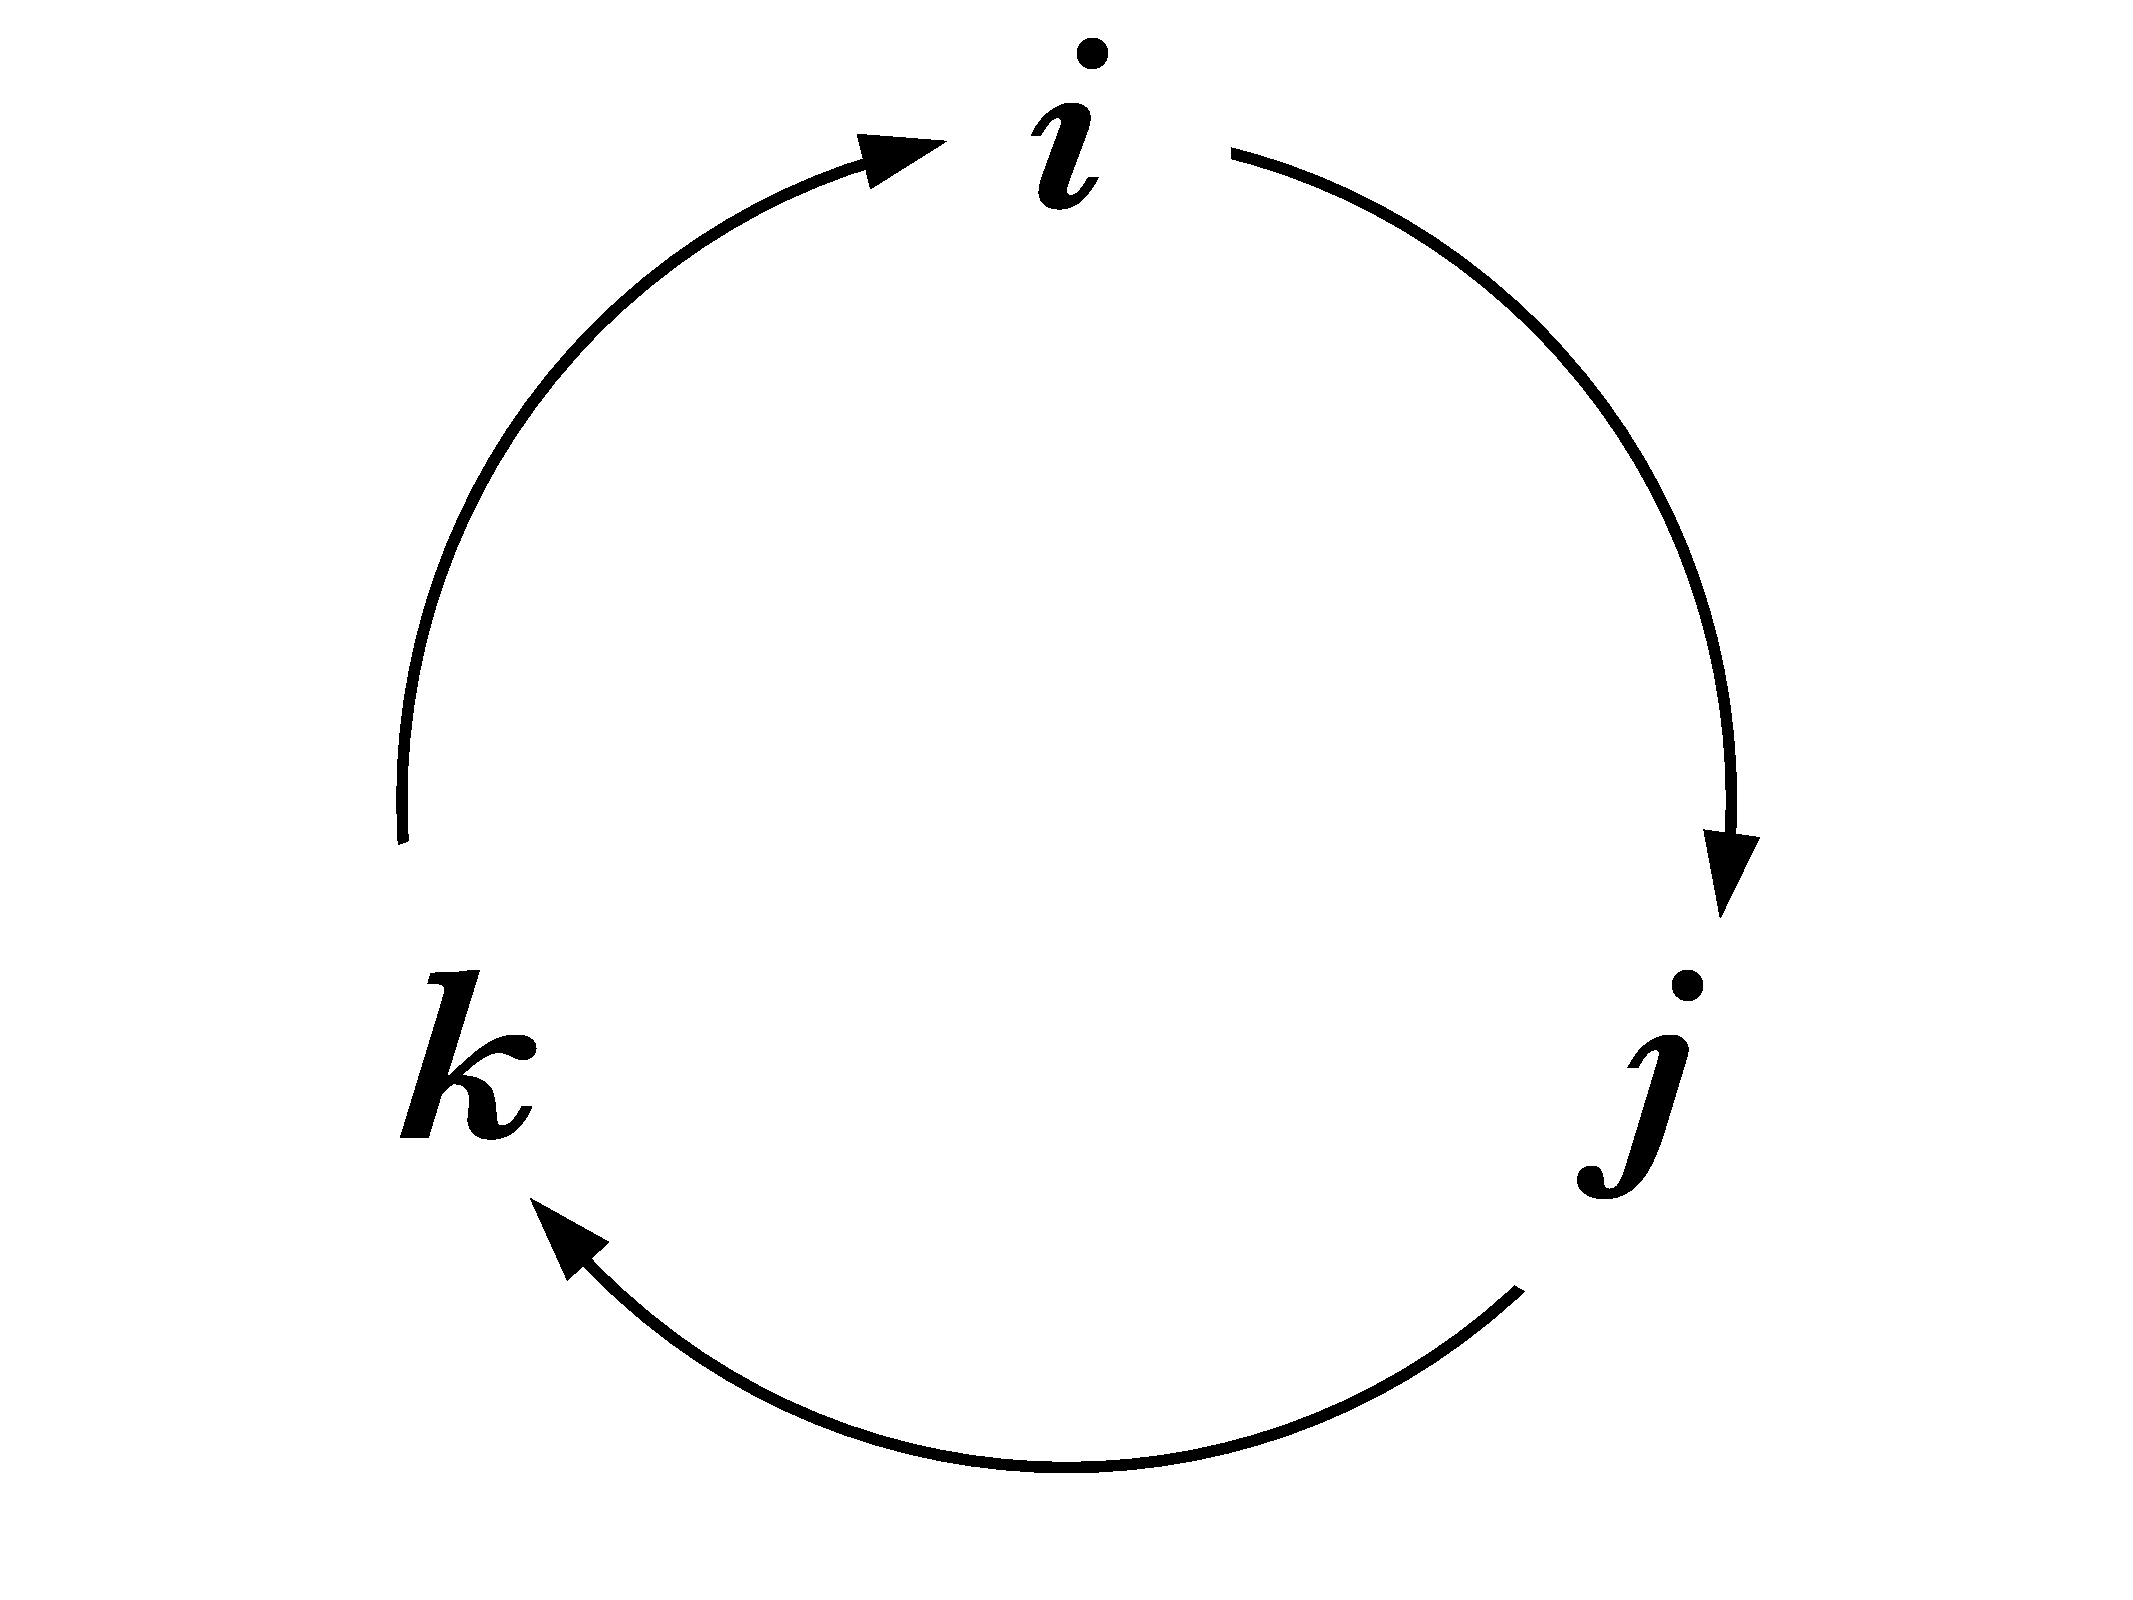
\includegraphics[width=0.2\linewidth]{Figures/quaternion_multiplication.pdf}
	\caption{Diagrama ilustrando a regra de multiplica\c c\~ao entre as unidades imagin\'arias $ \qi $, $ \qj $ e $ \qk $.}
	\label{fig:quatmult}
\end{figure}

% Moreover, $\qi$, $\qj$ and $\qk$ behave under the usual product in the same way the orthonormal base of $\mathbb{R}^3$ does with respect to the cross product, i.e. 

% \begin{equation}
% \mu_1 \mu_2 = \mu_3
% \end{equation}

% \noindent if and only if $(\mu_1, \mu_2, \mu_3)$ is a cyclical permutation of $(\qi, \qj, \qk)$ and

% \begin{equation}
% \mu_1 \mu_2 = -\mu_3
% \end{equation}

% \noindent otherwise.

Pode-se compreender $\qi, \qj$ e $\qk$ como unidades imagin\'arias ortogonais, gerando o espa\c co (tridimensional) das \emph{partes imagin\'arias} dos quat\'ernios,
\begin{equation}
\qV (q) = b\qi + c\qj + d\qk.
\end{equation}
A \emph{parte real} de um quat\'ernio \emph{q} \'e, naturalmente, definida como
\begin{equation}
S(q) = a.
\end{equation}

A parte imagin\'aria \'e comumente tamb\'em chamada de \emph{parte vetorial}, enquanto a parte real pode ser referida como \emph{parte escalar}. Um quat\'ernio com parte real nula \'e dito \emph{puro} --- o conjunto dos quais pode ser representado por $\qV(\mathbb{H})$ ---, e pode-se definir o produto vetorial entre quat\'ernios puros em analogia \`aquele usado em $\mathbb{R}^3$, i.e se $v_1 = b_1\qi + c_1\qj + d_1\qk$ e $v_2 = b_2\qi + c_2\qj + d_2\qk$, ent\~ao
\begin{equation}
v_1 \times v_2 = 
\begin{vmatrix}
\qi & \qj & \qk\\ 
b_1 & c_1 & d_1\\ 
b_2 & c_2 & d_2
\end{vmatrix}.
\end{equation}

Pela semelhan\c ca entre o conjunto $ \mathbb{R}^3 $, munido do produto vetorial, e o conjunto dos quat\'ernios puros, munido do produto vetorial entre quat\'ernios, eventualmente iremos nos referir a $\qi, \qj$ e $\qk$ como \emph{eixos}. O termo invoca a interpreta\c c\~ao destas unidades imagin\'arias como sendo eixos coordenados do espa\c co tridimensional de quat\'ernios puros.

A analogia com as opera\c c\~oes vetoriais em $\mathbb{R}^3$ aplica-se tamb\'em \`a defini\c c\~ao de produto interno entre quat\'ernios puros $v_1 = b_1\qi + c_1\qj + d_1\qk$ e $v_2 = b_2\qi + c_2\qj + d_2\qk$, a saber,
\begin{equation}
\langle v_1, v_2 \rangle =
b_1 b_2 + c_1 c_2 + d_1 d_2.
\end{equation}

A soma e o produto entre quat\'ernios permitem a distributividade (do produto em rela\c c\~ao \`a soma) e a associatividade, bastando respeitar as rela\c c\~oes em (\ref{eq:fund_rel}). Ou seja, se $q_1 = a_1 + b_1\qi + c_1\qj + d_1\qk$ e $q_2 = a_2 +  b_2\qi + c_2\qj + d_2\qk$, ent\~ao a soma \'e simplesmente dada por
\begin{equation}
q_1 + q_2 = (a_1 + a_2) + (b_1 + b_2)\qi + (c_1 + c_2)\qj + (d_1 + d_2)\qk,
\end{equation}
enquanto o produto \'e
\begin{equation}
\label{eq:q_prod}
\begin{aligned}
q_1 q_2 = &  \ (a_1 + b_1\qi + c_1\qj + d_1\qk) (a_2 +  b_2\qi + c_2\qj + d_2\qk)  \\ 
= & \ (a_1 a_2 - b_1 b_2 - c_1 c_2 - d_1 d_2)  \\
& + \qi (b_1 a_2 + a_1 b_2 - d_1 c_2 + c_1 d_2)  \\
& + \qj (c_1 a_2 + d_1 b_2 + a_1 c_2 - b_1 d_2)  \\
& + \qk (d_1 a_2 - c_1 b_2 + b_1 c_2 + a_1 d_2).
\end{aligned}
\end{equation}

Finalmente, pode-se notar que o produto entre quat\'ernios em  (\ref{eq:q_prod}) pode ser escrito em termos das partes escalar e vetorial, como
\begin{equation}
\label{eq:prod_vectors}
\begin{aligned}
q_1 q_2 = & \ S(q_1)S(q_2) - \langle\qV(q_1), \qV(q_2)\rangle \\
& + S(q_1) \qV(q_2) + S(q_2)\qV(q_1) + \qV(q_1) \times \qV(q_2).
\end{aligned}
\end{equation}
Da falta de comutatividade no produto vetorial, v\^e-se nesta equa\c c\~ao mais uma demonstra\c c\~ao de que o produto entre quat\'ernios \'e n\~ao-comutativo.

A conjuga\c c\~ao de um quat\'ernio $ q $, assim como nos complexos, \'e obtida pela troca de sinal de sua parte vetorial, $ \bar{q} \overset{\Delta}{=} S(q) - V(q) $. A defini\c c\~ao de norma, por sua vez, assemelha-se \`a de vetores em $ \mathbb{R}^4 $: $ |q| \overset{\Delta}{=} \sqrt{a^2 + b^2 + c^2 + d^2} $. Do exposto, e de (\ref{eq:prod_vectors}), percebe-se que $ |q|^2 = \bar{q} q = q \bar{q} $. Um quat\'ernio \'e \emph{unit\'ario} se $ |q| = 1 $, e o inverso de um quat\'ernio \'e encontrado em termos de seu conjugado e norma atrav\'es de
\begin{equation}
q^{-1} = \frac{\bar{q}}{|q|^2}.
\end{equation}

Da analogia entre os quat\'ernios puros e os elementos de $ \mathbb{R}^3 $, \'e natural falar em \emph{perpendicularidade} entre quat\'ernios puros. Dados $ \qmu,  \qnu \in \qV(\mathbb{H})$, percebe-se que s\~ao \emph{ortogonais} (i.~e. est\~ao associados a vetores ortogonais de $ \mathbb{R}^3 $) --- escreve-se $ \qmu \perp \qnu $ --- se e somente se
\begin{equation}
S(\qmu \qnu) = \langle \qmu, \qnu \rangle = 0.
\tag{$ \iff \qmu \perp \qnu $}
\end{equation}
Uma vez que, para dois quat\'ernios puros, unit\'arios e ortogonais $ \qmu $ e $ \qnu $, tem-se de (\ref{eq:prod_vectors}) que $ \qmu \qnu  = \qmu \times \qnu$, ent\~ao $ \qmu \qnu \perp \qmu $ e $ \qmu \qnu \perp \qnu $. Como $ (\qmu, \qnu, \qmu \qnu) $ \'e uma tripla de quat\'ernios puros, unit\'arios e ortogonais, eles formam uma base para $ \qV (\mathbb{H}) $. \'E poss\'ivel, portanto, reescrever (\ref{eq:q}) como
\begin{equation}
\label{eq:quat_generalizado}
q = a + b'\qmu + c'\qnu + d'\qmu \qnu,
\end{equation}
$a, b', c', d' \in \mathbb{R}$,
que representa um \emph{quat\'ernio generalizado}. Os ditos \emph{quat\'ernios de Hamilton} s\~ao aqueles escritos em termos da base can\^onica $ (1, \qi, \qj, \qk) $.


Al\'em da forma cartesiana em (\ref{eq:q}), os quat\'ernios permitem dois tipos de formas polares. A \emph{forma de Euler} \cite{ell2014quaternion} de um quat\'ernio \'e comumente expressa como
\begin{equation}
\label{eq:euler}
q = |q| e^{\qmu \theta} = |q|\cos \theta + |q|\qmu \sen \theta,
\end{equation}
em que $ \qmu $ \'e um quat\'ernio puro unit\'ario, paralelo \`a parte vetorial de $ q $.

Outra forma polar encontrada na literatura \cite{flamant2017time} \'e
\begin{equation}
q = |q| \exp (\qi \theta) \exp (-\qk \chi) \exp (\qj \varphi),
\end{equation}
em que os par\^ametros de fase, chamados de \^angulos de Euler, s\~ao \emph{quase unicamente} definidos sob o intervalo $ (\theta, \chi, \varphi) \in [-\pi/2, \pi/2] \times [-\pi/4, \pi/4] \times [-\pi, \pi[ $. Quando $ \chi = \pm \pi/4 $, o que equivale ao fen\^omeno do \emph{gimbal lock}, a fase do quat\'ernio n\~ao \'e bem definida.

Como consequ\^encia de (\ref{eq:euler}), \'e importante notar que todo quat\'ernio unit\'ario puro \'e uma raiz quadrada da unidade. Seja, por exemplo, o quat\'ernio unit\'ario puro $ \mathbf{\nu} $. De (\ref{eq:euler}),
\begin{equation}
%\label{key}
\mathbf{\nu} = |\mathbf{\nu}| e^{\mathbf{\nu} \theta},
\end{equation}
mas como $ |\mathbf{\nu}| = 1 $, ent\~ao
\begin{equation}
%\label{key}
\mathbf{\nu} = e^{\mathbf{\nu} \theta} \Rightarrow \theta = \pi,
\end{equation}
portanto,
\begin{equation}
%\label{key}
\mathbf{\nu}^2 = \left( e^{\mathbf{\nu}\pi} \right)^2 = e^{\mathbf{\nu} 2\pi} = 1.
\end{equation}

Esta propriedade de todo quat\'ernio puro unit\'ario $ \qmu $ leva ao fato de que os n\'umeros da forma $ a + \qmu b  $ formam um conjunto isomorfo aos n\'umeros complexos. Por esta raz\~ao, representaremos este conjunto por $ \mathbb{C}_{\qmu} \overset{\Delta}{=} \{ a + \qmu b \ |\  a, b \in \mathbb{R} \}$ ($ \mathbb{C}_{\qi} $ indica, portanto, o conjunto usual dos complexos).

Todo quat\'ernio $ q = a + b\qi + c\qj + d\qk \in \mathbb{H} $ pode ser representado segundo sua \emph{decomposi\c c\~ao simpl\'etica},
\begin{equation}
q = q^{(s)} + q^{(p)} \qj, \quad q^{(s)}, q^{(p)} \in \mathbb{C}_{\qi},
\end{equation}
em que $ q^{(s)} = a + b\qi $ e $ q^{(p)} = c + d\qi $ s\~ao frequentemente chamados de parte \emph{simplex} e \emph{perplex}, respectivamente. Perceba que essas duas componentes s\~ao n\'umeros complexos usuais. De forma geral, a decomposi\c c\~ao pode ser feita ao longo de um eixo diferente de $ \qi $: sejam $ \qmu $ e $ \qnu $ quat\'ernios puros unit\'arios e \emph{ortogonais}, ent\~ao o quat\'ernio $ q $ pode ser decomposto como
\begin{equation}
\label{eq:decomposicao}
q = q^{(s)} + q^{(p)} \qnu, \quad q^{(s)}, q^{(p)} \in \mathbb{C}_{\qmu}.
\end{equation}
Esta decomposi\c c\~ao tem grande import\^ancia no c\'alculo da QDFT (se\c c\~ao \ref{sec:QFT}) e na an\'alise de matrizes quaterni\^onicas (ca\'itulo \ref{ch:QGSP}).

Dois quat\'ernios $ q $ e $ r $ s\~ao ditos \emph{similares} se existe um quat\'ernio n\~ao-nulo $ v $ tal que $ v^{-1}q v = r $. Neste caso, pode-se escrever $ q \sim r $. A similaridade \'e uma rela\c c\~ao de equival\^encia entre quat\'ernios \cite{zhang1997quaternions}, e pode-se notar que todos os elementos de uma mesma classe de equival\^encia possuem a mesma norma, pois $ |v^{-1}q v| = |v^{-1}| \cdot |q| \cdot |v| = |q| $. Importa mencionar uma valiosa propriedade das transforma\c c\~oes de similaridade entre quat\'ernios, respons\'avel por sua grande aplica\c c\~ao na mec\^anica e na ind\'ustria da computa\c c\~ao gr\'afica. Trata-se da opera\c c\~ao de rota\c c\~ao no espa\c co 3D: dados $ v,x \in \mathbb{H} $, $ v = |v| e^{\qmu \alpha}$, a transforma\c c\~ao de similaridade
\begin{equation}
\label{eq:rotacao}
\phi_v(x) = v x v^{-1}
\end{equation}
produz a rota\c c\~ao da parte vetorial (imagin\'aria) de $ x $ em torno do eixo $ \qmu $ (que tem a mesma dire\c c\~ao da parte vetorial de $ v $) de um \^angulo $ 2\alpha $ \cite{ward2012quaternions}, seguindo a regra da m\~ao direita.

\section{A transformada de Fourier quaterni\^onica}
\label{sec:QFT}

Ao considerar-se sinais de valores quaterni\^onicos, a literatura contempla algumas ferramentas para seu processamento, como um operador gradiente \cite{jiang2014general} e algoritmos de filtragem adaptativa \cite{jiang2013frequency}. Nesta se\c c\~ao, no entanto, o foco ser\'a dado \`a transformada de Fourier quaterni\^onica (QFT, \emph{quaternion Fourier transform}), base para a an\'alise espectral de fun\c c\~oes hipercomplexas.

Seja $f$ uma fun\c c\~ao de valores quaterni\^onicos $f: \mathbb{R} \rightarrow \mathbb{H}$ e $\qmu \in \qV(\mathbb{H})$, $\qmu^2 = -1$. A QFT unidimensional \emph{\`a esquerda} pode ser definida pela fam\'ilia de transformadas
\begin{equation}
\mathcal{F}^L_{\mp \qmu}[f](\omega) = 
F^L_{\mp \qmu}(\omega) \overset{def}{=}
\kappa_{-} \int_{-\infty}^{\infty} e^{\mp \qmu \omega t} f(t) \mathrm{d}t.
\tag{QFT 1D \`a esquerda}
\end{equation}

Pode-se provar que a opera\c c\~ao inversa existe e \'e dada por
\begin{equation}
\mathcal{F}^{-L}_{\pm \qmu}[F^L](t) = 
f(t) =
\kappa_{+} \int_{-\infty}^{\infty} e^{\pm \qmu \omega t} F^L(\omega) \mathrm{d}\omega.
\tag{QFT 1D \`a esquerda inversa}
\end{equation}

Nas express\~oes acima, o quat\'ernio puro unit\'ario $\qmu$ indica o \emph{autoeixo} do n\'ucleo da transformada, \'e a unidade imagin\'aria de refer\^encia. Seu sinal no n\'ucleo da transformada \'e arbitr\'ario, bastando que as transforma\c c\~oes direta e inversa contenham sinais opostos. As constantes reais $\kappa_{-}$ e $\kappa_{+}$ satisfazem
\begin{equation}
\kappa_{+} \kappa_{-} = \frac{1}{2\pi},
\end{equation}
\noindent e se $\kappa_{-} = \kappa_{+}$, a transformada \'e dita unit\'aria.

%Similarly, the right-sided QFT pair is given by
%
%\begin{equation}
%\mathcal{F}^R_{\mp \mu}[f](\omega) = 
%F^R_{\mp \qmu}(\omega) \overset{def}{=}
%\kappa_{-} \int_{-\infty}^{\infty}  f(t) e^{\mp \qmu \omega t}  \mathrm{d}t.
%\tag{1D right-sided QFT}
%\end{equation}
%
%\begin{equation}
%\mathcal{F}^{-R}_{\pm \mu}[F^R](t) = 
%f(t) =
%\kappa_{+} \int_{-\infty}^{\infty} F^R(\omega) e^{\pm \qmu \omega t}  \mathrm{d}\omega.
%\tag{Inverse 1D right-sided QFT}
%\end{equation}
%
%
%Let $f_s, f_p \in \mathbb{C}_{\qmu}$ be respectively the simplex and perplex parts of the quat\'ernio-valued function $f(t)$, with respect to the unit quat\'ernio $\qnu$ so that $\qnu \perp \qmu$. Hence 
%
%\begin{align*}
%F^L(\omega) &= \kappa_{-} \int_{-\infty}^{\infty}
%e^{- \qmu \omega t} f(t) \mathrm{d}t \\
%& = 
%\kappa_{-} \int_{-\infty}^{\infty}
%e^{- \qmu \omega t} f_s(t) \mathrm{d}t +
%\kappa_{-} \int_{-\infty}^{\infty}
%e^{- \qmu \omega t} f_p(t) \mathrm{d}t \qnu \\
%&= \underbrace{F^L_s (\omega)}_{\isomorphism CTFT} + \underbrace{F^L_p (\omega)}_{\isomorphism CTFT} \qnu,
%\end{align*}
%
%\noindent that is, the QFT may be computed using two continuous-time Fourier Transforms (CTFT) subsequent to symplectic decomposition of the function transformed function.

Da mesma forma como foi definida a transformada \`a esquerda, pode-se tratar da transformada \`a direita, alterando a posi\c c\~ao relativa entre a fun\c c\~ao $ f(t) $ e o n\'ucleo. O leitor deve perceber que, no caso em que o autoeixo coincide com $ \qi $, a QFT coincide com a transformada de Fourier de tempo
%\footnote{Por raz\~oes hist\'oricas, o termos \emph{tempo} e \emph{frequ\^encia} ser\~ao utilizados para se referir, respectivamente, aos dom\'inios da fun\c c\~ao original e da fun\c c\~ao transformada, muito embora em alguns cen\'arios as vari\'aveis livres n\~ao tenham tais significados (e.g. no processamento de imagens).}
cont\'inuo.

Nesta pesquisa, ter\'a mais relev\^ancia a vers\~ao da QFT em que os dom\'inios de origem e de destino da transformada s\~ao discretos, a QDFT unidimensional de eixo $ \qmu $, como definida em \cite[sec. 3.3.1]{ell2014quaternion}. Se $ \qmu $ \'e um quat\'ernio unit\'ario puro qualquer, a $ m $-\'esima componente do vetor transformado pela QDFT unit\'aria de eixo $ \qmu $ \`a esquerda \'e dada por
\begin{equation}
\label{eq:QDFT_fwd}
\widehat{v}_m = \text{QDFT}\{ \mathbf{v} \}_m \overset{\Delta}{=} \frac{1}{\sqrt{N}} \sum_{n=0}^{N-1}  \exp \left( -\qmu \frac{2\pi}{N} nm \right) v_n \in \mathbb{C}_{\qmu},
\end{equation}
com a f\'ormula da transforma\c c\~ao inversa trazendo a m\'ultiplica\c c\~ao pelo n\'ucleo tamb\'em \`a esquerda:
\begin{equation}
\label{eq:QDFT_inv}
v_n = \text{QDFT}^{-1}\{ \widehat{\mathbf{v}} \}_n = \frac{1}{\sqrt{N}}\sum_{m=0}^{N-1}  \exp \left( \qmu \frac{2\pi}{N} nm \right) \widehat{v}_m.
\end{equation}

As equa\c c\~oes de an\'alise e s\'intese podem ser escritas em forma matricial como
\begin{equation}
\label{eq:QDFT}
\widehat{\mathbf{v}} = \text{QDFT}\{ \mathbf{v} \} = \mathbf{F} \mathbf{v},
\end{equation}
\begin{equation}
\label{eq:QDFT_mtx_inv}
\mathbf{v} = \text{QDFT}^{-1}\{ \widehat{\mathbf{v}} \} = \mathbf{F}^{-1} \widehat{\mathbf{v}},
\end{equation}
em que $ \mathbf{F} $ \'e a matriz da transformada unit\'aria,
%--multiplicando sempre \`a esquerda--,
com entradas $ \{\mathbf{F}\}_{n,m} = \sqrt{N}^{-1} \exp \left( -\qmu \frac{2\pi}{N} nm \right)$. Uma vez que  $ \exp \left( -\qmu \frac{2\pi}{N} \right) $ \'e uma raiz $ N $-\'esima da unidade, assim como $ \exp \left( -\qi \frac{2\pi}{N} \right) $, segue que a matriz $ \mathbf{F} $ da QDFT compartilha muitas da propriedades da matriz da DFT, dentre elas a inversibilidade, o que garante a validade de (\ref{eq:QDFT_inv}) e  (\ref{eq:QDFT_mtx_inv}).
%A equa\c c\~ao de s\'intese segue diretamente do fato de que $ \mathbf{F} $ \'e invers\'ivel ($ \{\mathbf{F}^{-1}\}_{n,m} = e^{\qmu \frac{2\pi}{N} nm}$): $ \mathbf{v} = \mathbf{F}^{-1} \widehat{\mathbf{v}} $.

A decomposi\c c\~ao simpl\'etica, apresentada em (\ref{eq:decomposicao}), pode ser aplicada a cada quat\'ernio de uma matriz quaterni\^onica e, assim, gerar uma matriz \emph{simplex} e outra \emph{perplex}. Utilizando este princ\'ipio, Ell e Sangwine \cite{ell2014quaternion} demonstraram que a QDFT de um sinal $ \mathbf{x} = [x_0, x_1, \dots, x_{N-1}] \in \mathbb{H}^N $ poderia ser facilmente computada via duas DFT complexas, ao utilizar a decomposi\c c\~ao simpl\'etica de cada amostra do sinal ao longo do mesmo eixo que a QDFT,
%. Relembrando a eq. (\ref{eq:QDFT_fwd}),
\begin{equation}
\begin{aligned}
%\label{eq:QDFT_fwd}
\text{QDFT}\{ \mathbf{x} \}_m &= \frac{1}{\sqrt{N}} \sum_{n=0}^{N-1} \exp \left( -\qmu \frac{2\pi}{N} nm \right) x_n \\
&= \frac{1}{\sqrt{N}} \sum_{n=0}^{N-1} \exp \left( -\qmu \frac{2\pi}{N} nm \right) (x_n^{(s)} + x_n^{(p)}\qnu) \\
&= \text{DFT}_{\qmu}\{ \mathbf{x}^{(s)} \}_m +
\text{DFT}_{\qmu}\{ \mathbf{x}^{(p)} \}_m \qnu,
\end{aligned}
\end{equation}
em que $ \text{DFT}_{\qmu} $ indica a DFT calculada com n\'umeros complexos tendo $ \qmu $ por unidade imagin\'aria. Do ponto de vista computacional, pode-se usar os mesmos algoritmos para o c\'alculo da DFT convencional.

Esta breve apresenta\c c\~ao da QDFT ilustra que
\begin{itemize}[noitemsep]
\item embora as componentes de frequ\^encia sejam sinais quaterni\^onicos, as frequ\^encias s\~ao reais,
\item a estrutura da QDFT assemelha-se bastante \`a da DFT usual, permitindo at\'e mesmo o aproveitamento dos seus algoritmos para comput\'a-la. Esta semelhan\c ca de estruturas ser\'a aproveitada para investigar a fracionariza\c c\~ao da QDFT, no cap\'itulo \ref{ch:FrQDFT}.
\end{itemize}

Para uma introdu\c c\~ao completa aos quat\'ernios e sua aplica\c c\~ao ao processamento de sinais, recomenda-se \cite{zhang1997quaternions,ell2014quaternion,flamant2017time, jiang2014general}.

\section{Princ\'ipios do processamento de sinais sobre grafos}
\label{sec:GSPintro}

Em diversos contextos, os sinais de interesse est\~ao naturalmente definidos sobre uma estrutura em rede, modelada como um grafo. Sejam medi\c{c}\~oes em um conjunto de sensores e dispositivos de Internet das Coisas~\cite{alam2015toward,guo2016qos,ma2016non,yu2016novel}, informa\c c\~oes de posi\c c\~ao e cor sobre um \emph{mesh} 3D para computa\c c\~ao gr\'afica \cite{nguyen2014compression}, ou mesmo sinais de resson\^ancia magn\'etica funcional (fMRI, \emph{functional magnetic resonance imaging}) sobre redes cerebrais \cite{goldsberry2017brain,leonardi2013tight}, s\~ao todos exemplos de aplica\c c\~oes em que os dados obtidos est\~ao intimamente ligados \`a topologia da rede sobre a qual est\~ao definidos. Em todos estes cen\'arios, e muitos outros, GSP tem encontrado espa\c co para expandir a teoria e propor solu\c c\~oes. Nesta se\c c\~ao, pretende-se cobrir brevemente os fundamentos de GSP.


Um sinal $ \mathbf{s} $ sobre um grafo $ \mathcal{G} = \{\mathcal{V}, \mathbf{A}\} $, com $ |\mathcal{V}| = N $, \'e definido como uma fun\c c\~ao discreta que mapeia $\mathcal{V}$ em um conjunto de grandezas escalares, usualmente os n\'umeros complexos ou reais,
\begin{equation}
%\label{key}
s: \ \mathcal{V} \rightarrow \mathbb{C} \ | \ s(v_i) = s_i,
\end{equation}
de modo que um sinal definido sobre $ \mathcal{G} $ \'e um vetor em $ \mathbb{C}^N $ \emph{indexado pelos v\'ertices de} $ \mathcal{G} $. A matriz de adjac\^encia $ \mathbf{A} $ traz em sua entrada $ A_{ij} $ o peso da aresta indo de $ v_j $ para $ v_i $. Uma vez que se determina uma rotula\c c\~ao e ordem espec\'ifica para os elementos de $ \mathcal{V} = \{v_1, \dots, v_N\}$, n\~ao h\'a ambiguidade em representar o sinal como o vetor $ \mathbf{s} = (s_0 \ s_1 \ \dots \ s_{N-1})^T$, $ s_i \in \mathbb{C} $, $ 0 \leq i \leq N-1 $. Representa-se por $ \mathcal{S} $ o espa\c co de sinais definidos sobre um certo grafo $ \mathcal{G} = \{\mathcal{V}, \mathbf{A}\} $.

A Fig.~\ref{fig:graphs} traz exemplos de representa\c c\~oes de sinais sobre grafos, nos quais a rotula\c c\~ao dos v\'ertices \'e impl\'icita (associa-se a amostra $ s_i $ ao v\'ertice $ v_i $). Os valores das amostras dos sinais podem ser indicados \emph{numericamente}, junto aos v\'ertices (Figs. \ref{figa_graphs} e \ref{figb_graphs}), ou por meio de uma escala de cores (Fig.~\ref{figd_graphs}). Ao longo desta se\c c\~ao, ser\'a priorizado o uso desta \'ultima representa\c{c}\~ao.%Por ora, o leitor pode ter-se indagado sobre a pr\'opria \emph{constru\c c\~ao} do grafo para o caso de sinais reais, como aquele obtido de medi\c c\~oes de temperatura na Fig. \ref{figd_graphs}, o que de fato n\~ao \'e uma quest\~ao trivial e ser\'a abordada na subse\c c\~ao a seguir.

\begin{figure}
	\centering
	\subfloat[\label{figa_graphs}]{
		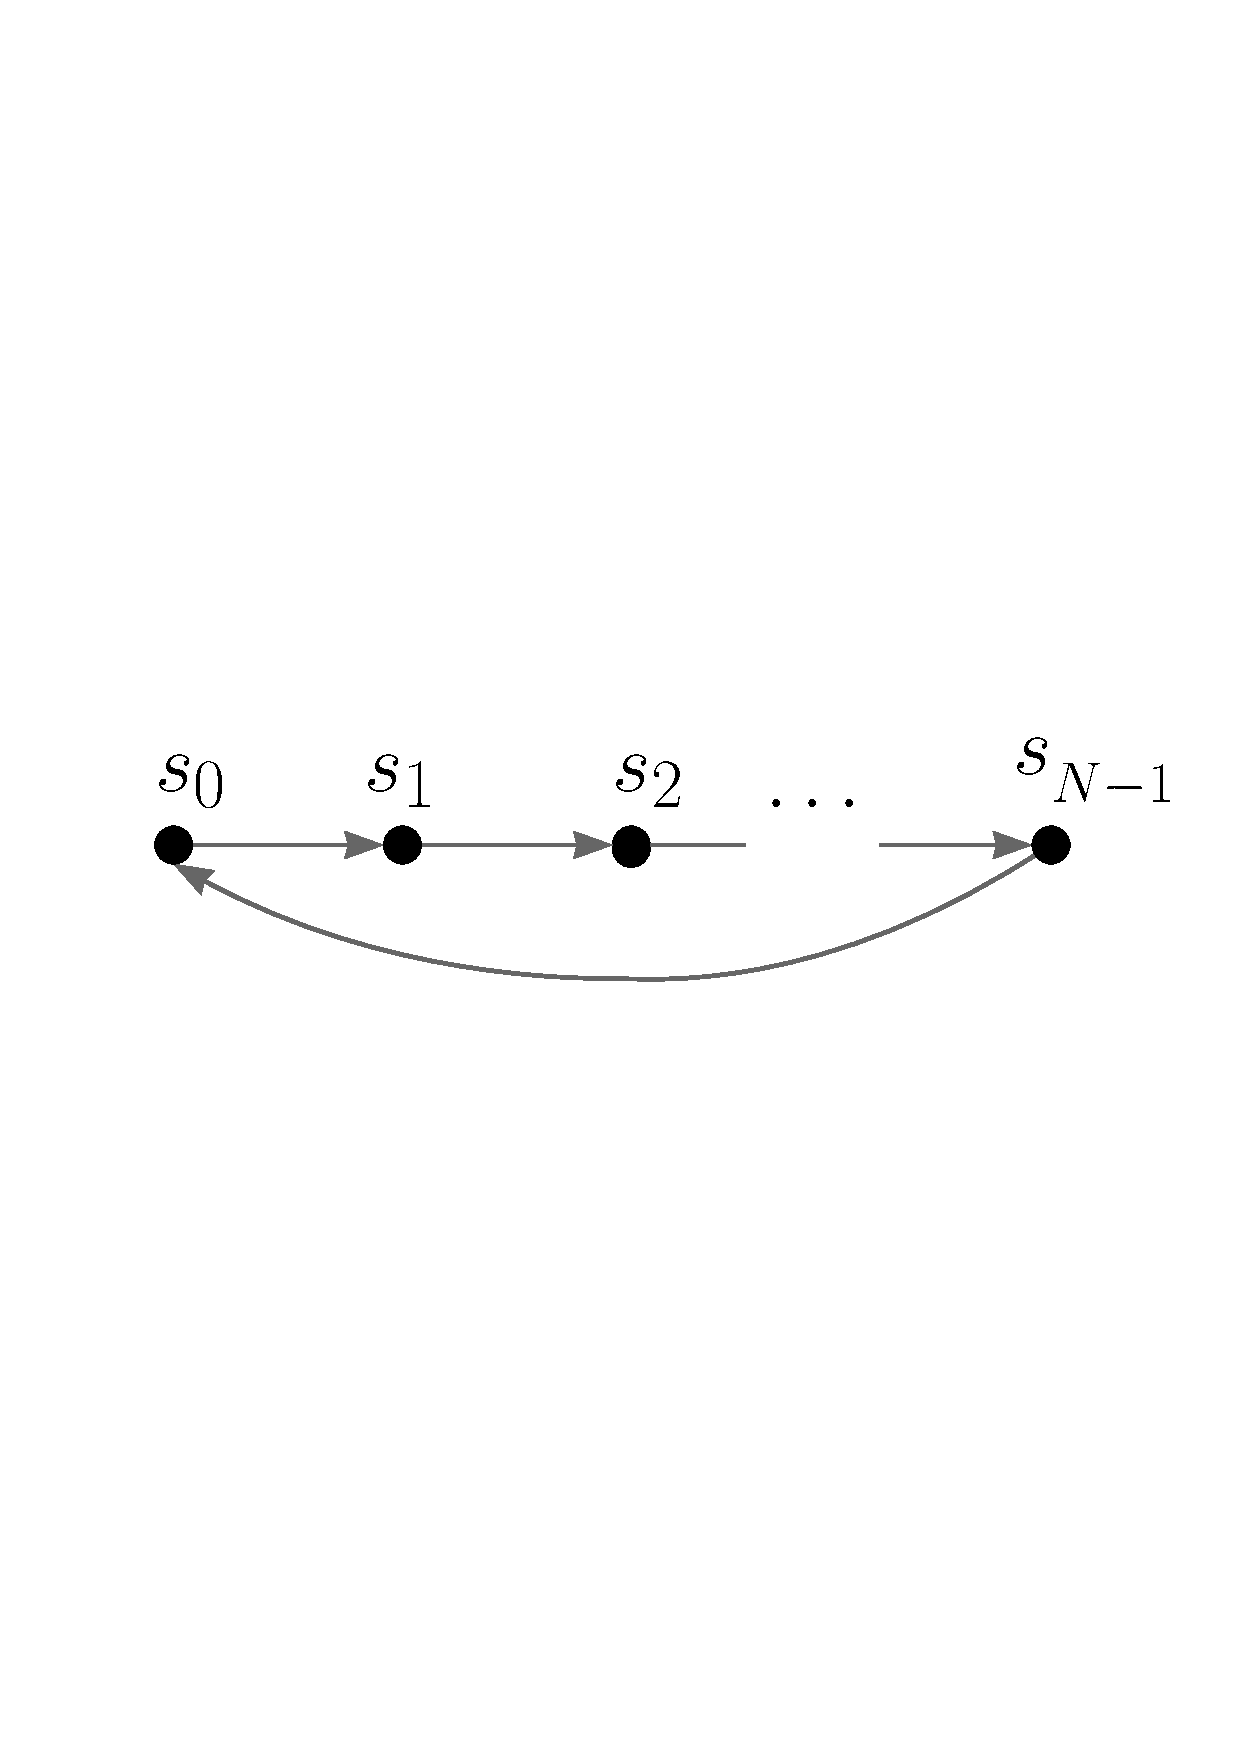
\includegraphics[width=0.25\linewidth]{Figures/signal_ring_graph_white_border.pdf}
	}
	\subfloat[\label{figb_graphs}]{
		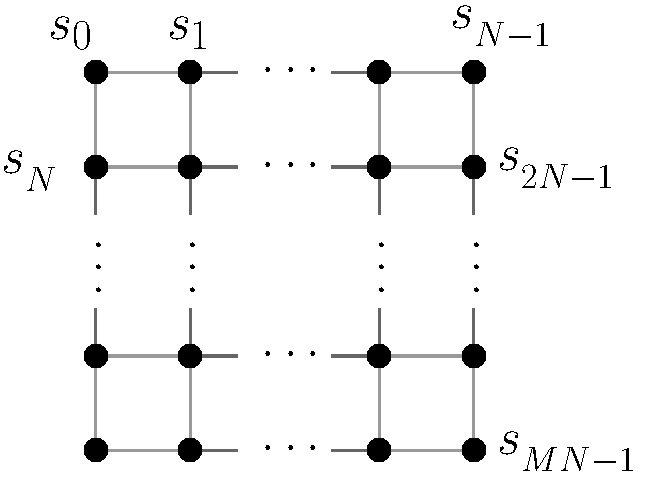
\includegraphics[width=0.25\linewidth]{Figures/image_graph.pdf}
	}%
	\subfloat[\label{figd_graphs}]{
		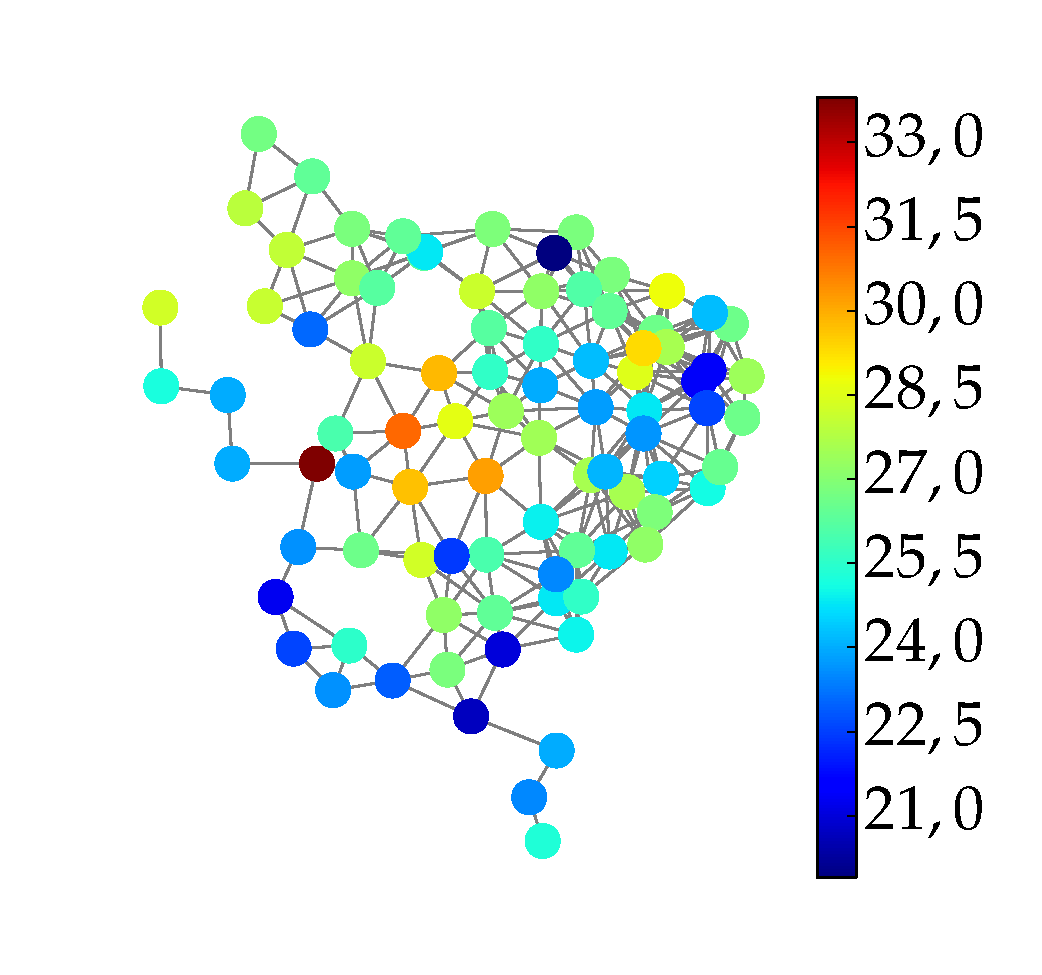
\includegraphics[width=0.26\linewidth]{Figures/temp_NE_stretched.pdf} }%
	\caption{Representa\c{c}\~oes de sinais sobre (a) um grafo em anel direcionado, (b) um grafo em grade retangular uniforme  e (c) um grafo formado por cidades do Nordeste brasileiro.}%
	\label{fig:graphs}%
	%	\vspace{-0.9cm}
	%	{\\ \small Fonte: o autor.}
\end{figure}

Um sinal de comprimento finito e de tempo discreto \'e modelado pelo grafo em anel direcionado (considera-se os pesos unit\'arios), como mostrado na Fig.~\ref{figa_graphs}: a no\c c\~ao de evolu\c c\~ao temporal \'e capturada pelas arestas direcionadas; a periodicidade imposta pelas condi\c c\~oes de fronteira da an\'alise de Fourier de tempo discreto \'e modelada pela aresta realimentando a \'ultima amostra \`a primeira. O grafo na Fig. \ref{figb_graphs} \'e um modelo para imagens digitais \cite{sandryhaila2012nearest} chamado \emph{nearest-neighbor}, em que a depend\^encia entre pixels \'e aproximada para existir apenas entre vizinhos, e o grafo na Fig. \ref{figd_graphs} \'e um exemplo de grafo de rede de sensores\footnote{Quando n\~ao \'e especificado em contr\'ario, chama-se \emph{grafo de (rede de) sensores} um grafo conectado com v\'ertices distribu\'idos uniformemente numa regi\~ao do espa\c co euclidiano bidimensional.}, com pesos das arestas dados pelo inverso da dist\^ancia euclidiana, sobre o qual definiu-se o sinal da temperatura \`a meia-noite de 01 de fevereiro de 2012 em cidades do Nordeste brasileiro\footnote{Fonte: Banco de Dados Meteorol\'ogicos para Ensino e Pesquisa (BDMEP) do Instituto Nacional de Meteorologia. Acesso gratuito, dispon\'ivel em: \url{http://www.inmet.gov.br/portal/index.php?r=bdmep/bdmep}}.

As caracter\'isticas espectrais de um sinal dependem fortemente do dom\'inio sobre o qual ele \'e definido. %, mas n\~ao faz sentido reconhecer essa depend\^encia em Processamento Cl\'assico de Sinais porque nele trabalha-se apenas com dom\'inios regulares e uniformes\footnote{Mesmo quando se aborda \emph{amostragem n\~ao-uniforme}, as t\'ecnicas desenvolvidas ainda visam \`a \emph{recupera\c{c}\~ao} do sinal em um dom\'inio -- de tempo -- tipicamente regular.}.
Em geral, diz-se que um sinal cont\'em majoritariamente baixas frequ\^encias se amostras \emph{adjacentes} t\^em valores \emph{pr\'oximos}, e altas frequ\^encias se t\^em valores \emph{d\'ispares}. Considerando sinais definidos sobre grafos, fica evidente que a no\c c\~ao de amostras adjacentes depende da topologia do grafo em quest\~ao, e portanto \emph{um mesmo sinal pode apresentar espectros distintos se definido sobre grafos diferentes}. 
%A Fig. \ref{fig:diff_struct} confirma essa intui\c c\~ao, apresentando o espectro de um sinal segundo a base de autovetores da matriz Laplaciana do grafo, para dois grafos distintos; na Fig. \ref{fig:diff_struct_b}, as amostras de maior valor s\~ao adjacentes \`aquelas de menor valor, o que causa componentes de maior frequ\^encia do que se o grafo usado como dom\'inio fosse um anel a pesos constantes (Fig. \ref{fig:diff_struct_a}).

%Em 2006, P\"uschel e Moura publicaram sua teoria de processamento alg\'ebrico de sinais (ASP, do ingl\^es \emph{algebraic signal processing}) \cite{moura2006algebraic}. A descrição de sinais e filtros do ponto de vista alg\'ebrico \'e intencionalmente abstrata e gen\'erica: tanto os filtros como os sinais s\~ao simplesmente elementos de espa\c cos vetoriais dotados de multiplica\c c\~ao e distributividade. Especificamente, o espa\c co de filtros \'e uma \emph{\'algebra}, sobre a qual toma-se um \emph{m\'odulo} para ser o espa\c co de sinais. Uma descri\c c\~ao detalhada sobre ASP foge ao escopo deste cap\'itulo, mas o leitor interessado pode tirar bastante proveito dos trabalhos originais de P\"uschel e Moura \cite{puschel2008time,puschel2008space}.
%
%O aspecto de ASP que levou ao processamento sobre grafos, o que de fato nos interessa diretamente, \'e que o espa\c co de filtros \'e \emph{gerado} pelo operador de atraso unit\'ario de sinais. Um exemplo tornar\'a a afirma\c c\~ao menos obscura: seja a \'algebra polinomial $ \mathbb{C}[x] / (x^N - 1) $, ou $ {A}  = \{ \sum_{\ell=0}^{N-1} a_\ell x^\ell | a_\ell \in \mathbb{C} \}$, que consiste em todos os polin\^omios de coeficientes complexos com grau menor do que $ N $, dotados da adi\c c\~ao e multiplica\c c\~ao polinomiais usuais, m\'odulo $ x^N - 1 $. \'E comum representar sinais e filtros de tempo discreto e comprimento $ N $ como elementos de $ {A}  $, caso em que a convolu\c c\~ao c\'iclica torna-se a simples multiplica\c c\~ao polinomial modular. Por exemplo, o sinal $ \mathbf{s}_1 = (0 \ \ 2 \ \ 1 \ \ 0) $ \'e representado por $ s_1(x) = x^2 + 2x $, e sua vers\~ao deslocada de uma unidade, $ \mathbf{s}_2 = (0 \ \ 0 \ \ 2 \ \ 1) $, \'e dada por $ s_2(x) = x^3 + 2x^2 $. Fica claro que, neste caso, o filtro de atraso unit\'ario \'e $ d(x) = x $, cujas pot\^encias \emph{geram} a base $ (1, x, x^2, \dots, x^{N-1}) $ para o espa\c co de filtros. Esta rela\c c\~ao se mant\'em para qualquer \'algebra em ASP; portanto, Moura certamente concluiu que, ao definir um operador de deslocamento unit\'ario para sinais sobre grafos, isto daria in\'icio \`a constru\c c\~ao da teoria de GSP.

Um conceito fundamental em GSP \'e o de operador de deslocamento. Trata-se de uma matriz quadrada $ S $ extra\'ida a partir do grafo $ \mathcal{G} $, tal que $ S_{ji} $ somente pode ser n\~ao-nulo se $ i = j $ ou $ (v_i, v_j) $ for uma aresta de peso n\~ao-nulo de $ \mathcal{G} $ \cite{segarra2015interpolation}. Escolhas usuais para $ S $ s\~ao a matriz de adjac\^encia \cite{sandryhaila2014big} e a Laplaciana \cite{shuman2013emerging}, embora outras op\c c\~oes existam (e.g. \cite{girault2015translation, dees2019unitary}), a depender de qual propriedade se deseje. O restante da se\c c\~ao tomar\'a a matriz de adjac\^encia como operador de deslocamento, por ser aquele que mais claramente transmite a no\c c\~ao de atraso unit\'ario do sinal no grafo. Pode-se ver que a multiplica\c c\~ao de um sinal $ \mathbf{x} $ \`a esquerda por $ \mathbf{A} $ faz com que cada amostra $ x_i $ seja redistribu\'ida para os v\'ertices vizinhos, ponderada pelo peso das arestas que saem do v\'ertice $ i $:
\begin{equation}
y_j = \sum_{i=0}^{N-1} A_{ij} x_i.
\end{equation}

O conceito fica ainda mais claro ao se tomar o grafo em anel direcionado com pesos unit\'arios, modelo para o dom\'inio de tempo discreto (Fig. \ref{figa_graphs}). Pode-se ver que sua matriz de adjac\^encia,
\begin{equation}\label{eq:C}
\mathbf{C} =
\left[\renewcommand{\arraystretch}{0.65}\begin{array}{cccc}
&  &  &   1\\ 
1 &  &   & \\ 
&   \ddots &  & \\ 
&  &   1 & 
\end{array}\right],
\end{equation}
\noindent realiza precisamente o papel de atraso num sinal de tempo discreto. Ou seja, se um sinal $ \mathbf{s} = (s_1 \ s_2 \ \dots \ s_N)^T $ definido em um grafo em anel \'e multiplicado \`a  esquerda por $ \mathbf{C} $, tem-se
\begin{equation}\label{eq:graph_shift_C}
\mathbf{s}^{\langle 1 \rangle} = \mathbf{C} \mathbf{s},
\end{equation}
com $ \mathbf{s}^{\langle 1 \rangle} = (s_N \ s_1 \ \dots \ s_{N-1})^T $.
Para um sinal $ \mathbf{x} $ sobre um grafo qualquer $ \mathcal{G} = \{\mathcal{V}, \mathbf{A}\} $, $ \mathbf{A} $ age como um \emph{filtro} de atraso (ou deslocamento) sobre $ \mathbf{x} $, e a vers\~ao deslocada deste sinal \'e representada por $ \mathbf{x}^{\langle 1 \rangle} = \mathbf{A} \mathbf{x}$.

%e a opera\c c\~ao de deslocamento do sinal,
%\begin{equation}
%%\label{key}
%\widetilde{\mathbf{x}} = \mathbf{A} \mathbf{x} \Rightarrow \widetilde{x}_i = \sum_{j=0}^{N-1} A_{i,j} x_j,
%\end{equation}
%significa substituir o valor em cada v\'ertice do grafo pela soma dos valores adjacentes, ponderada pelos pesos das arestas incidentes. No dom\'inio do tempo discreto, o deslocamento \'e a mera transfer\^encia c\'iclica de valor das amostras porque o grafo subjacente \'e em anel a pesos constantes (Fig. \ref{figa_graphs}).

\subsection{Filtros sobre grafos}
\label{subsec:filtros}

Observar a matriz de adjac\^encia como um filtro levou \`a defini\c c\~ao de um filtro de sinais sobre grafos como sendo qualquer matriz $ \mathbf{H} \in \mathbb{C}^{N \times N} $ \cite{sandryhaila2013filters}, visto que o produto matriz-vetor sempre resulta num vetor (ou \emph{filtro} $ \times $ \emph{sinal} $ = $ \emph{sinal}). Isso implica que os filtros sobre grafos s\~ao sempre lineares, uma vez que a distributividade da multiplica\c c\~ao em rela\c c\~ao \`a adi\c c\~ao matricial garante que
\begin{equation}
%\label{key}
\mathbf{H} (\alpha_1 \mathbf{x}_1 + \alpha_2 \mathbf{x}_2) =  \alpha_1 \mathbf{H} \mathbf{x}_1 + \alpha_2 \mathbf{H}  \mathbf{x}_2.
\end{equation}

A propriedade de invari\^ancia no tempo (ou ao deslocamento) requer que $ \mathbf{A} \mathbf{H} \mathbf{x} = \mathbf{H} \mathbf{A} \mathbf{x} {,} \ \forall \mathbf{x}$. Uma classe de filtros que sempre obedece a esse requisito s\~ao aqueles na forma de um polin\^omio $ h(\cdot) $ avaliado em $ \mathbf{A} $,
\begin{equation}
\label{eq:filter_poly}
h(\mathbf{A}) = \sum_{\ell=0}^{L-1} h_\ell \mathbf{A}^\ell,
\end{equation}
com $ L$ menor ou igual ao grau do polin\^omio m\'inimo $ m_\mathbf{A} $ de $ \mathbf{A}$~\cite{sandryhaila2013discrete,sandryhaila2014big}. Assim, estes filtros LSI s\~ao uma s\'erie de pot\^encias finita no operador de deslocamento, exatamente como ocorre em processamento cl\'assico de sinais de tempo discreto, em que os filtros LTI t\^em representa\c c\~ao em termos de polin\^omios em $ z^{-1} $, pela transformada Z. A menos que dito em contr\'ario, ser\'a utilizado o termo ``filtro LSI`` como sin\^onimo para um filtro como (\ref{eq:filter_poly}).

\subsection{A transformada de Fourier sobre grafos}

Uma vez que a transformada de Fourier de um sinal \'e a sua proje\c{c}\~ao em uma base de fun\c{c}\~oes invariantes \`a  filtragem linear e invariante no tempo (LTI, do ingl\^es \emph{linear and time-invariant}) \cite{oppenheim1997signals}, em GSP define-se a transformada de Fourier sobre grafos (GFT, do ingl\^es \emph{graph Fourier transform}) como a decomposi\c{c}\~ao de um sinal em termos de uma base de autovetores do operador de deslocamento --- e, portanto, autovetores da filtragem LSI~\cite{sandryhaila2013gft}.

Seja $ \mathbf{A} $ a matriz de adjac\^encia de um grafo de $ N $ v\'ertices. Se $ \mathbf{A} $ for diagonaliz\'avel, tem-se\footnote{Se $\mathbf{A}$ n\~ao for diagonaliz\'avel, o racioc\'inio pode ser repetido utilizando-se a forma can\^onica de Jordan.}
\begin{equation}\label{eq:gft_01}
\mathbf{A} = \mathbf{V} \mathbf{\Lambda} \mathbf{V}^{-1},
\end{equation}
em que $ \mathbf{V} $ cont\'em os $ N $ autovetores de $ \mathbf{A} $ em suas colunas, isto \'e,
\begin{equation}\label{eq:gft_02}
\mathbf{V} = (\mathbf{v}_0 \ \mathbf{v}_1 \ \dots\ \mathbf{v}_{N-1}).
\end{equation}

Como filtros LSI s\~ao polin\^omios em $ \mathbf{A} $, as colunas de $ \mathbf{V} $ formam uma base de vetores invariantes \`a  filtragem LSI
%. Somando a isto o fato de que os subespa\c{c}os gerados pelos autovetores de um mesmo autovalor de $ \mathbf{A} $ s\~ao irredut\'iveis, t\^em interse\c{c}\~ao nula e suas dimens\~oes somam $ N $ \cite{sandryhaila2013gft}, $ \mathbf{V} $ fornece uma base invariante \`a  filtragem LSI
para o espa\c{c}o de sinais $ \mathcal{S} $ sobre o grafo com matriz de adjac\^encia $ \mathbf{A} $. Desta forma, um sinal $ \mathbf{x} \in \mathcal{S} $ pode ser decomposto em suas componentes na base $ \mathbf{V} $ como
\begin{align}\label{eq:GFT_inv}
\mathbf{x} &= \widehat{x}_0 \mathbf{v}_0 + \dots + \widehat{x}_{N-1} \mathbf{v}_{N-1} = \mathbf{V} (\widehat{x}_0 \ \widehat{x}_1 \ \dots \ \widehat{x}_{N-1})^T \notag \\
&= \mathbf{V} \widehat{\mathbf{x}},
\end{align}
e esta \'e definida como a equa\c{c}\~ao de s\'intese da \emph{transformada de Fourier sobre grafos}. A equa\c{c}\~ao de an\'alise da GFT \'e, portanto,
\begin{equation}\label{eq:GFT_fwd}
\widehat{\mathbf{x}} = \mathbf{V}^{-1} \mathbf{x}.
\end{equation}

Para sinais de tempo discreto, foi assinalado que seu dom\'inio \'e modelado como um grafo com matriz de adjac\^encia $ \mathbf{C} $ em~(\ref{eq:C}). Como $ \mathbf{C} $ \'e circulante, ela \'e diagonalizada pela matriz da transformada discreta de Fourier (DFT, do ingl\^es \emph{discrete Fourier transform}), dada por $ \mathbf{F} $, $ F_{n,k} = \exp \left( -\jmath\frac{2 \pi}{N} nk \right) $. Assim, pode-se escrever%, que cont\'em em suas linhas os autovetores da DFT. Atrav\'es do polin\^omio caracter\'istico de $ \mathbf{C} $,
%\begin{equation}
%\label{key}
%p_{\mathbf{C}}(\lambda) = \text{det} (\lambda \mathbf{I} - \mathbf{C}) =
%\begin{vmatrix}
%\lambda &  &  &   -1\\ 
%-1 & \lambda &   & \\ 
%&   \ddots & \ddots & \\ 
%&  &   -1 & \lambda
%\end{vmatrix}
%=\lambda^N - 1,
%\end{equation}
%mostra-se que seus autovalores s\~ao as $ N $ ra\'izes da unidade. Assim, a diagonaliza\c c\~ao da matriz $ \mathbf{C} $ pela matriz da DFT \'e escrita como
\begin{equation}\label{eq:diag_C}
\mathbf{C} = \mathbf{F}^{-1} \mathbf{\Lambda}_{\mathbf{C}} \mathbf{F},
\end{equation}
em que $\mathbf{\Lambda}_{\mathbf{C}}$ \'e uma matriz diagonal com os autovalores de $\mathbf{C}$. V\^e-se que a matriz da GFT, para grafos em anel, \'e $ \mathbf{V}^{-1} = \mathbf{F} $, o que resulta na desej\'avel propriedade de que a GFT de sinais de tempo discreto coincide com a  DFT, demonstrando consist\^encia com a teoria cl\'assica.

\subsection{O dom\'inio da frequ\^encia}

A defini\c c\~ao empregada para a GFT sugere interpretar os autovetores $ \mathbf{v}_i $ da matriz de adjac\^encia como as ``componentes de frequ\^encia'' associadas \`as \emph{frequ\^encias de grafo} representadas pelos autovalores $ \lambda_i $ (como a componente de Fourier $ {\text{e}}^{-\jmath \Omega t} $, no dom\'inio do tempo cont\'inuo $ t $, \'e associada \`a frequ\^encia $ \Omega $). A menos que os polin\^omios caracter\'istico e m\'inimo de $ \mathbf{A} $ sejam iguais, uma mesma frequ\^encia estar\'a associada a duas ou mais componentes linearmente independentes, como ocorreu com o sinal na Fig. \ref{fig:diff_struct_GSPA}. Na mesma figura, nota-se que, embora o sinal seja visualmente suave, seu espectro possui componentes associadas a autovalores de grande magnitude, o que levanta a quest\~ao de definir um crit\'erio coerente para se falar em \emph{altas} e \emph{baixas} frequ\^encias de sinais sobre grafos.


\begin{figure}
\centering
\begin{minipage}[c]{0.3\linewidth}
	\subfloat[\label{fig:diff_struct_a_GSPA}]{
		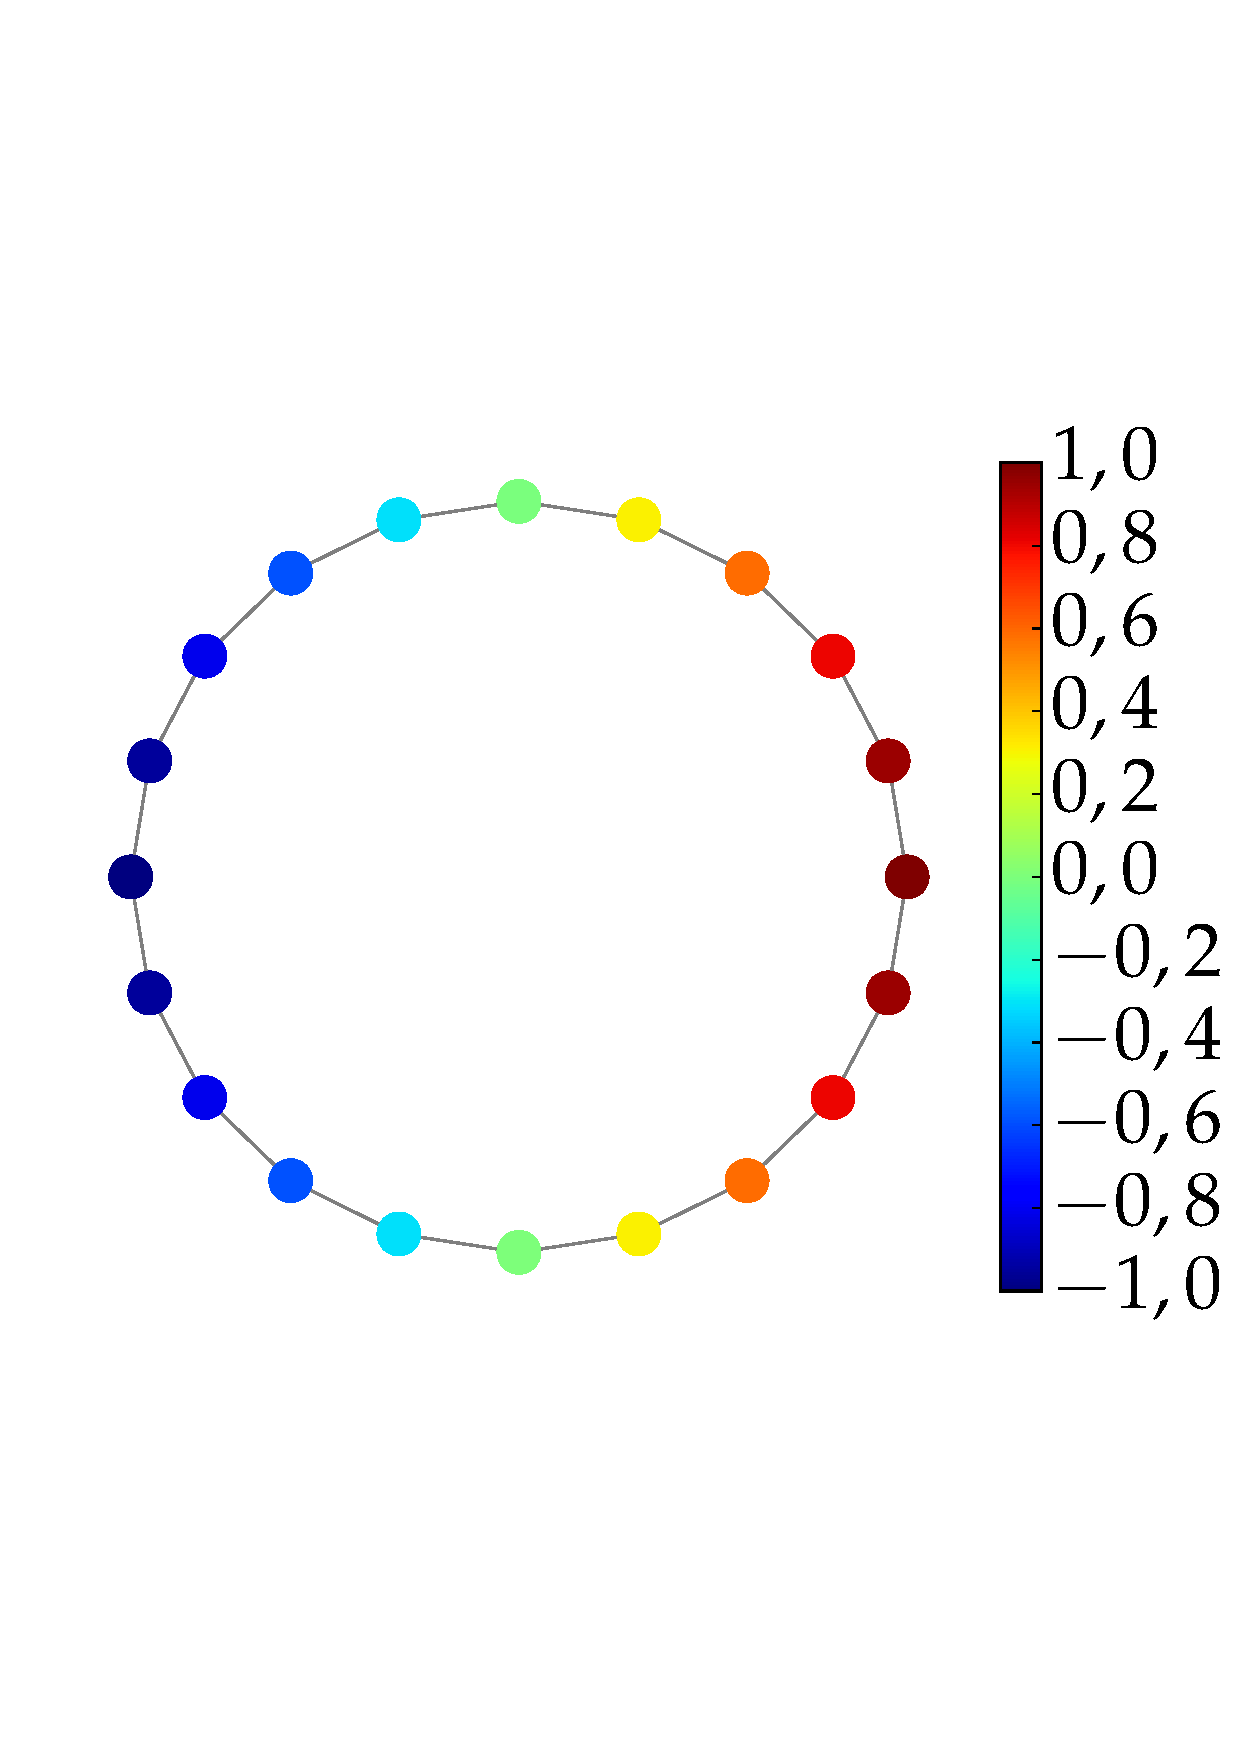
\includegraphics[width=\linewidth]{Figures/ring_different_structure_01_GSPA_larger.pdf}
	}
\end{minipage} %
\begin{minipage}[c]{0.27\linewidth}
	\subfloat[\label{fig:diff_struct_b_GSPA}]{
		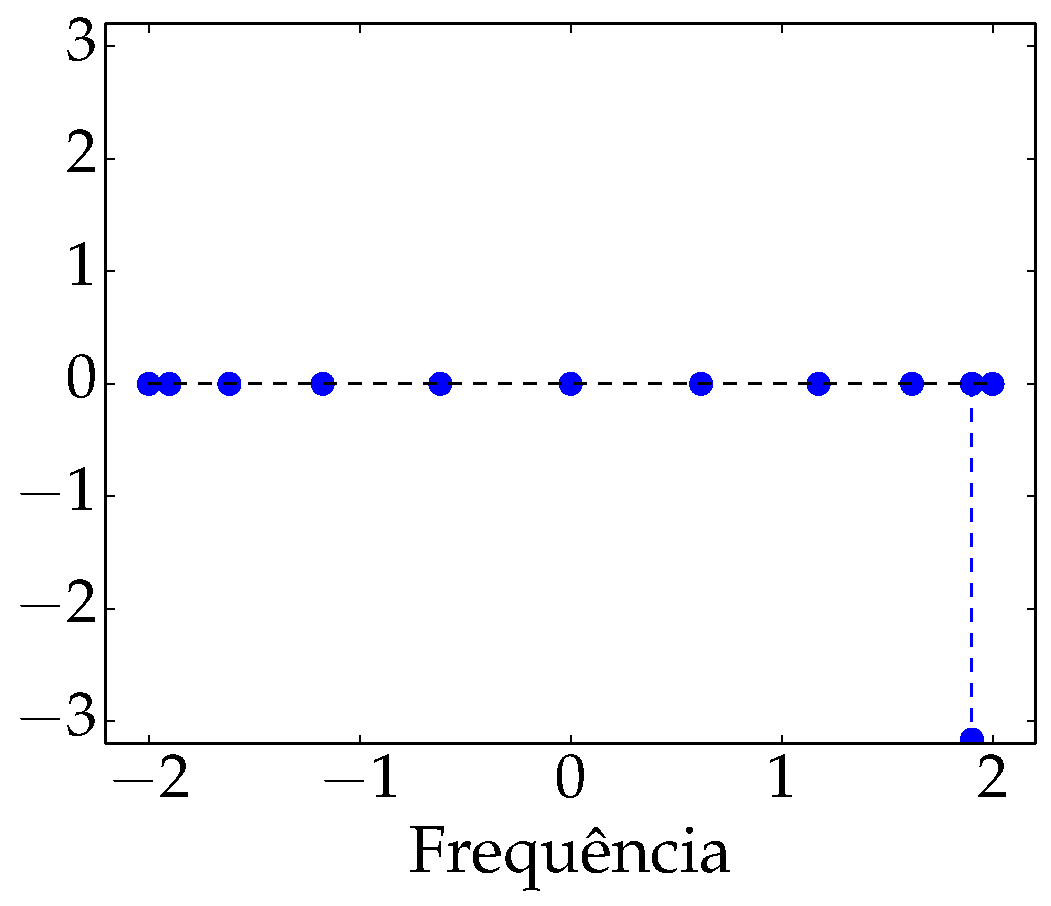
\includegraphics[width=\linewidth]{Figures/ring_different_structure_01_spectrum_GSPA_PT_2.pdf}
	}
\end{minipage}%
\caption{(a) Sinal sobre um grafo em anel n\~ao-direcionado e (b) seu espectro em GSP\textsubscript{A}.}%
\label{fig:diff_struct_GSPA}%
%	\vspace{-0.2cm}
%	{\\ \small Fonte: o autor.}
\end{figure}

Para fundamentar matematicamente a no\c c\~ao de frequ\^encia no contexto de GSP, partiu-se de uma m\'etrica usual para sinais de tempo discreto: a \emph{varia\c c\~ao total}, que calcula a soma das diferen\c cas entre amostras adjacentes de um sinal e, portanto, assume valores maiores para sinais de maior frequ\^encia. Sua express\~ao matem\'atica, para certo sinal de comprimento finito $ \mathbf{x} = (x_0 \ \ x_1 \ \ \dots \ \ x_{N-1}) $, \'e
\begin{equation}
\label{eq:TV}
TV(\mathbf{x}) = \sum_{n=0}^{N-1} | x_n - x_{n-1 \text{ mod } N}|.
\end{equation}

De (\ref{eq:C}) e (\ref{eq:graph_shift_C}), v\^e-se que (\ref{eq:TV}) pode ser reescrita em termos da norma $ \ell_1 $\footnote{A norma $ \ell_1 $ \'e um caso particular da norma $ \ell_p $ de um vetor $ \mathbf{x} \in \mathbb{C}^{N} $, definida como $ \Vert \mathbf{x}\Vert_p \overset{\Delta}{=} \left(\sum_{k=0}^{N-1} |x_k|^p\right)^{1/p} $. Quando n\~ao for explicitamente indicado, a nota\c c\~ao sem subscrito $ \Vert \cdot \Vert $ indica a norma $ \ell_2 $.} como $ TV(\mathbf{x}) = \Vert \mathbf{x} - \mathbf{C x}\Vert_1 $, utilizando a matriz de adjac\^encia do grafo em anel para realizar o deslocamento c\'iclico do sinal. Assim, uma generaliza\c{c}\~ao da fun\c c\~ao $ TV(\cdot) $ para sinais definidos sobre grafos quaisquer, i.~e., a \emph{varia\c c\~ao total sobre grafos} para um sinal $ \mathbf{s} $ sobre o grafo $ \mathcal{G} = \{\mathcal{V}, \mathbf{A}\} $, foi definida como
\begin{equation}
\label{eq:var_total}
TV_G(\mathbf{s}) \overset{\Delta}{=} \Vert \mathbf{s} - \mathbf{A}^{\text{\emph{norm}}} \mathbf{s}\Vert_1,
\end{equation}
com $ \mathbf{A}^{\text{\emph{norm}}} = |\lambda_{max}|^{-1}\mathbf{A} $ e $ \lambda_{max} $ o autovalor de $ \mathbf{A} $ com maior m\'odulo. A normaliza\c c\~ao de $ \mathbf{A} $ visa evitar a magnifica\c c\~ao excessiva das amostras do sinal deslocado \cite{sandryhaila2014frequency}.

\begin{figure}
	\centering
	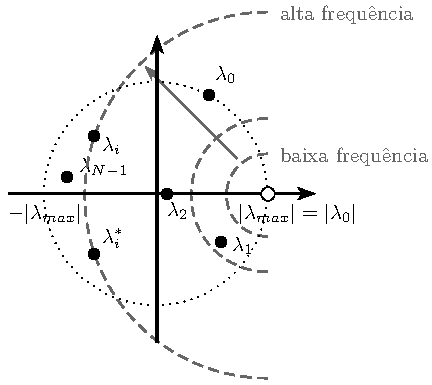
\includegraphics[width=0.35\linewidth]{Figures/graph_frequency.pdf}
	\caption{Ordenamento das frequ\^encias de sinais sobre grafos, de baixa para alta, no plano complexo. Fonte: adaptado de \cite{sandryhaila2014frequency}.}
	\label{fig:ordem_freq}
	%	{\\ \small Fonte: adaptado de \cite{sandryhaila2014frequency}.}
\end{figure}

Seja $ \mathbf{A} $ diagonaliz\'avel e com autovalores (possivelmente complexos) ordenados tais que
\begin{equation}
\label{eq:eig_order}
|\lambda_0| \leq |\lambda_1| \leq \dots \leq |\lambda_{N-1}| \overset{\Delta}{=} |\lambda_{max}|,
\end{equation}
associados aos autovetores $ (\mathbf{v}_i)_{i=0,\dots,N-1} $ escolhidos de modo que $ \Vert \mathbf{v}_k \Vert_1 = 1 $. Tomando a varia\c c\~ao total de um autovetor $ \mathbf{v}_k $ associado a $ \lambda_k $, tem-se
\begin{align*}
%\label{key}
TV_G(\mathbf{v}_k) &= \Vert \mathbf{v}_k - \mathbf{A} \mathbf{v}_k \Vert_1  = \Vert\mathbf{v}_k - \frac{1}{|\lambda_{max}|} \lambda_k \mathbf{v}_k \Vert_1 = \left|1 - \frac{\lambda_k}{|\lambda_{max}|}\right| \Vert \mathbf{v}_k \Vert_1 = \Big| \lambda_k - |\lambda_{max}| \Big| \frac{\Vert \mathbf{v}_k \Vert_{1}}{|\lambda_{max}|}
\end{align*}
de forma que, como foi feito $ \Vert \mathbf{v}_k \Vert_1 = 1 $, tem-se a equival\^encia
\begin{equation}
\label{eq:TV_ordering}
\Big|  \lambda_i - |\lambda_{max}|\Big| \leq \Big|  \lambda_j - |\lambda_{max}|\Big| \iff TV_G(\mathbf{v}_i) \leq TV_G(\mathbf{v}_j),
\end{equation}
ou seja, componentes de frequ\^encia associadas a autovalores mais pr\'oximos do ponto $ |\lambda_{max}| $ no plano complexo s\~ao mais suaves e s\~ao, portanto, ditas de \emph{baixa frequ\^encia}. A Fig. \ref{fig:ordem_freq} ilustra esse ordenamento para as frequ\^encias de grafos, o que esclarece a leitura do espectro do sinal na Fig. \ref{fig:diff_struct_a_GSPA}, cuja matriz de adjac\^encia tem autovalores reais.

%\begin{figure}
%\centering
%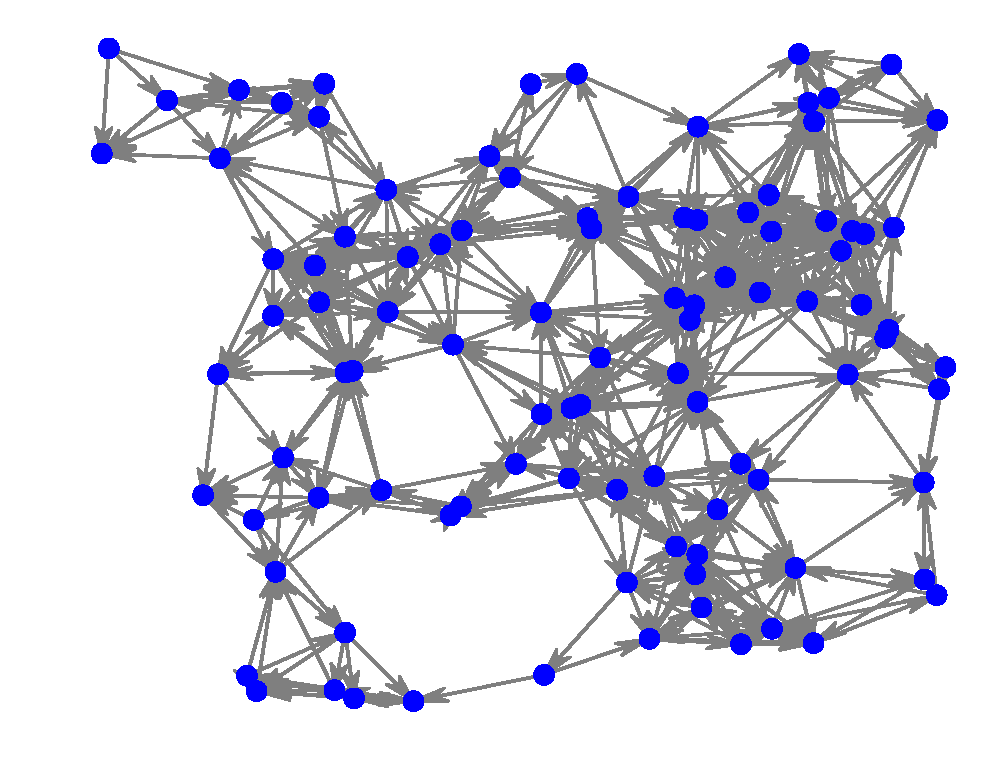
\includegraphics[width=0.35\linewidth]{Figures/showing_random_sensor_spectrum_directed_graph.pdf}
%\caption{Grafo de sensores direcionado, com 100 v\'ertices, sem la\c cos ou m\'ultiplas arestas.}
%\label{fig:directed_graph}
%%	{\\ \small Fonte: o autor.}
%\end{figure}
%
%\begin{figure}
%\centering
%\subfloat[]{
%	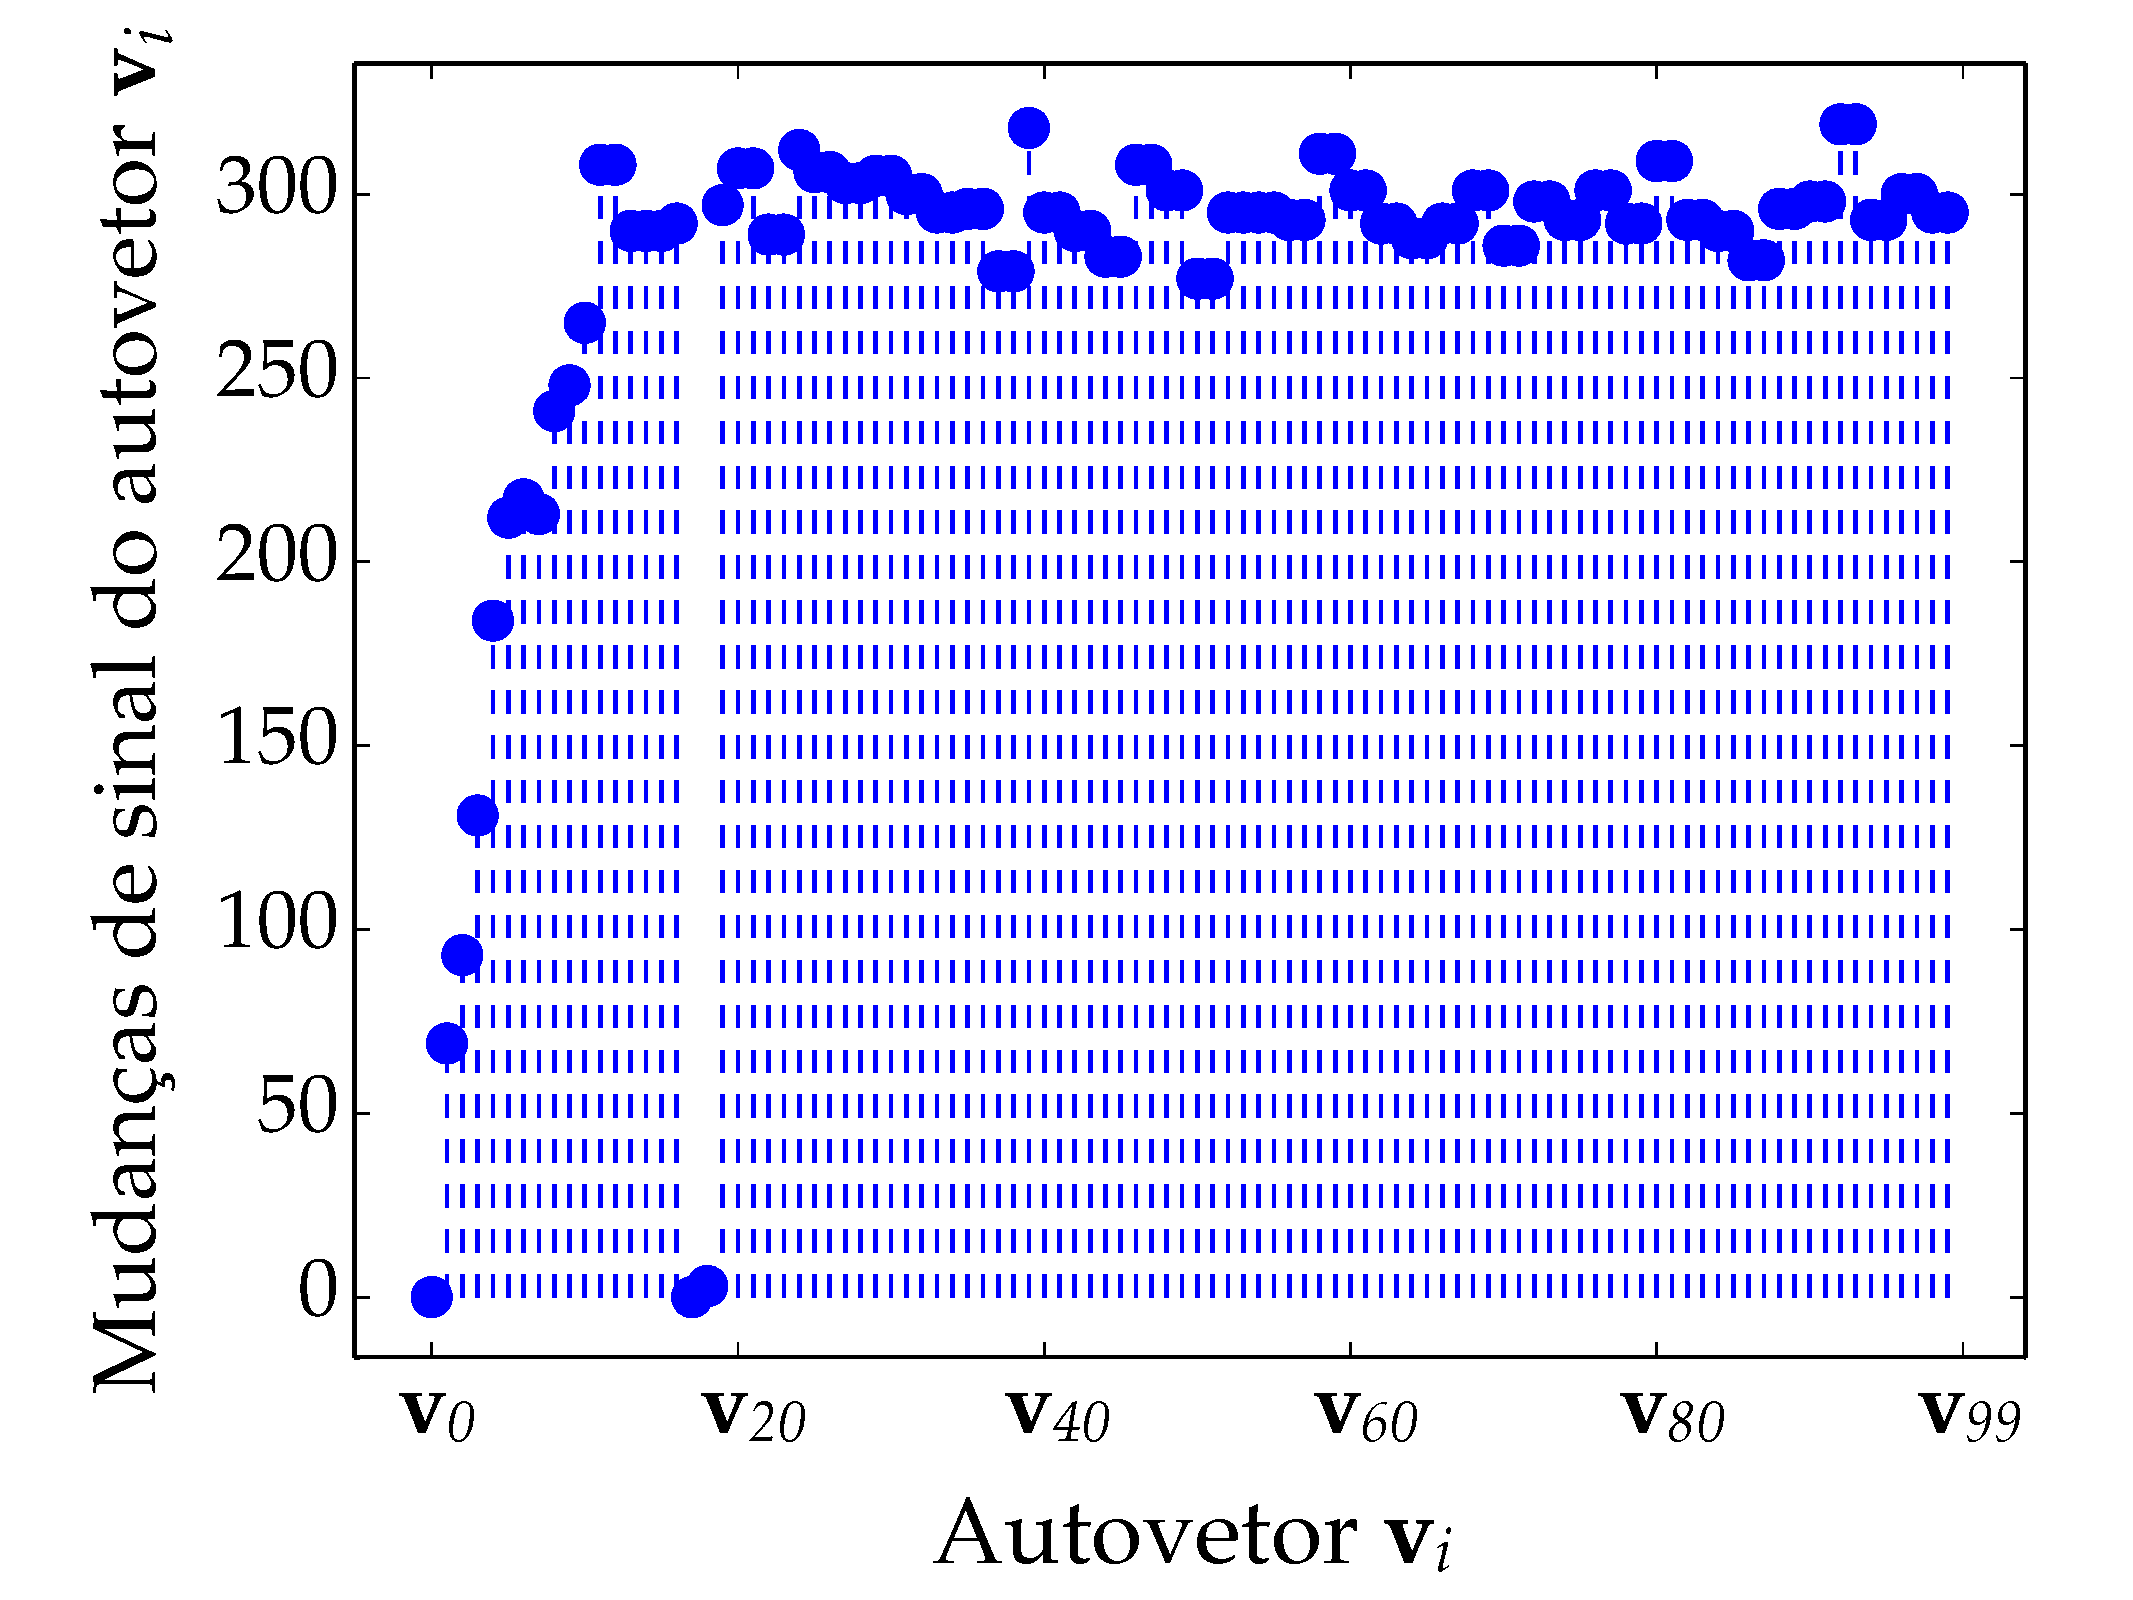
\includegraphics[width=0.4\linewidth]{Figures/showing_random_sensor_spectrum_directed_zero_crossings_1D_edited.pdf}
%}~
%\subfloat[\label{fig:showing_random_sensor_spectrum_directed_b}]{
%	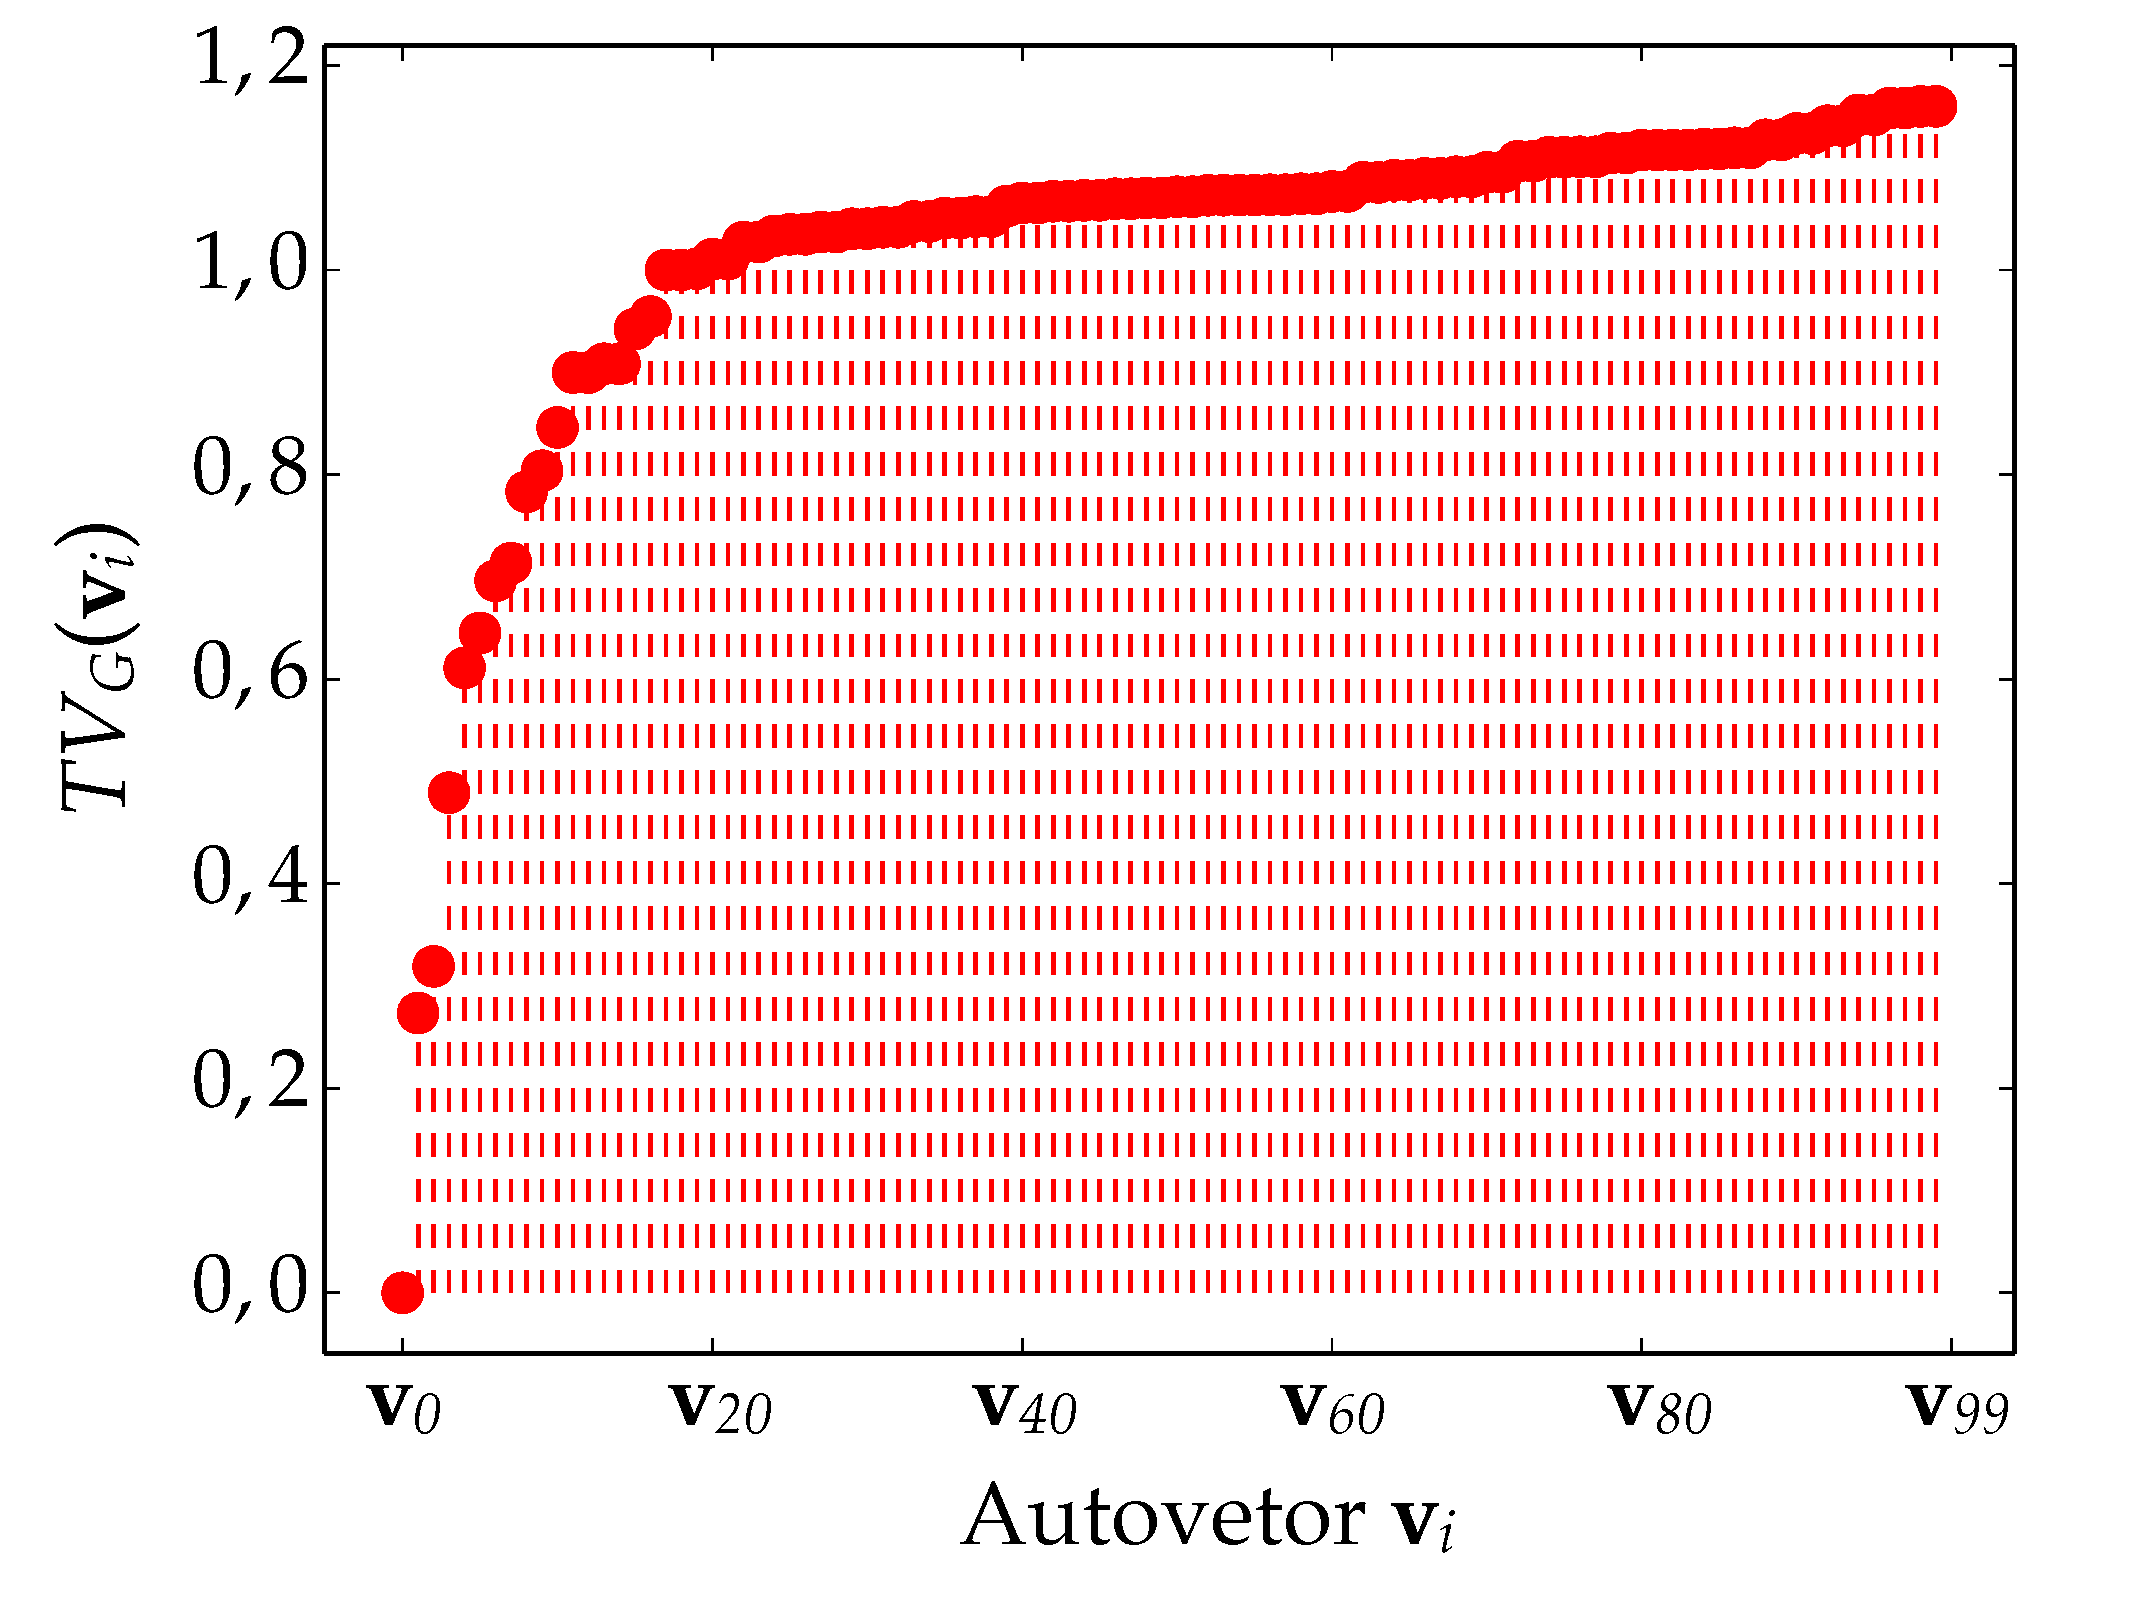
\includegraphics[width=0.4\linewidth]{Figures/showing_random_sensor_spectrum_directed_TV_1D_edited.pdf}
%}
%\caption{(a) N\'umero de mudan\c cas de sinal e (b) varia\c c\~ao total dos autovetores $ (\mathbf{v}_i)_{i=0,\dots,N-1} $ da matriz $ \mathbf{A} $, ordenados de modo que os respectivos autovalores se disponham do mais pr\'oximo ao mais distante do ponto real $ |\lambda_{max}| $ no plano complexo.}
%\label{fig:showing_random_sensor_spectrum_directed}
%%	{\\ \small Fonte: o autor.}
%\end{figure}
%
%Para verificar a consist\^encia desta no\c c\~ao de frequ\^encia, tomemos o grafo da Fig.~\ref{fig:directed_graph}. O n\'umero de mudan\c cas de sinal (n\'umero de arestas ligando v\'ertices com amostras de sinal distinto) e a varia\c c\~ao total $ TV_G $ de cada autovetor da matriz de adjac\^encia do grafo s\~ao mostrados na Fig.~\ref{fig:showing_random_sensor_spectrum_directed}. Ambas as m\'etricas visam quantificar a taxa de varia\c c\~ao de um sinal sobre o grafo, mas, uma vez que o n\'umero de mudan\c cas de sinal ignora as varia\c c\~oes que n\~ao cruzam o zero, a varia\c c\~ao total sobre grafos representa de forma mais fiel a medida de frequ\^encia em um sinal. A Fig.~\ref{fig:showing_random_sensor_spectrum_directed_b} mostra como $ TV_G(\mathbf{v}_k) $ cresce monotonicamente \`a medida que o respectivo autovalor de $ \mathbf{v}_k $, $ \lambda_k $, se afasta do ponto $ |\lambda_{max}| $ no plano complexo.


\chapter[Fracionariza\c c\~ao da QDFT]{Fracionariza\c c\~ao da transformada discreta de Fourier quaterni\^onica}
\label{ch:FrQDFT}

As transformadas lineares discretas s\~ao ferramentas basilares no campo de processamento de sinais. Entre as muitas classes em que elas se dividem, est\'a a das transformadas fracion\'arias, como a de Fourier, que encontra aplica\c c\~oes em an\'alise tempo-frequ\^encia, compress\~ao, impress\~ao de marca d'\'agua digital, entre outras \'areas \cite{bultheel2002shattered}. Em alguns poucos trabalhos, tamb\'em as transformadas quaterni\^onicas j\'a foram fracionarizadas
%, nos trabalhos de Xu, Wei e Roopkumar 
\cite{guanlei2008fractional, wei2013different, roopkumar2016quaternionic}, inclusive com implementa\c c\~oes e aplica\c c\~oes, como no uso em marcas-d'\'agua adaptativas por Chen
\cite{chen2018quaternion}. No entanto, nenhuma abordagem para fracionariza\c c\~ao de transformadas de Fourier discretas sobre quat\'ernios, de que este autor tenha conhecimento, partiu da an\'alise da sua autoestrutura. Ao explorar esta via, novos \textit{insights} te\'oricos e novas formas de implementa\c c\~ao podem surgir.

Este cap\'itulo traz uma contribui\c c\~ao deste projeto de tese, e est\'a dividido da seguinte forma.
%No presente artigo, \'e avaliada a autoestrutura da transformada discreta de Fourier quaterni\^onica (QDFT, \textit{quat\'ernio discrete Fourier transform}) unidimensional, a partir de um teorema que demonstra a rela\c c\~ao entre os autovetores da transformada discreta de Fourier (DFT, \textit{discrete Fourier transform}) e aqueles da QDFT. Em seguida, \'e proposta a fracionariza\c c\~ao da QDFT, com um ou m\'ultiplos par\^ametros, e um esquema de cifragem de imagens coloridas em PNG (\textit{portable network graphics}, formato com tr\^es camadas de cor e uma de opacidade) \'e apresentado, a fim de ilustrar a implementa\c c\~ao e aplica\c c\~ao da transformada fracion\'aria.
A se\c c\~ao \ref{sec:autoestrutura} relembra o leitor sobre a QDFT e demonstra o teorema central deste cap\'itulo, sobre o compartilhamento de autovetores entre a DFT e a QDFT. A se\c c\~ao \ref{sec:FrQDFT} define a vers\~ao fracion\'aria da QDFT, com base em sua autodecomposi\c c\~ao, e demonstra algumas de suas propriedades. A se\c c\~ao \ref{sec:multi} prop\~oe a extens\~ao multiparam\'etrica da QDFT fracion\'aria e aplica-a num esquema de cifragem de imagens coloridas com camada de opacidade. O cap\'itulo \'e conclu\'ido na se\c c\~ao \ref{sec:conclusao}.


%A diversidade significativa de transformadas lineares discretas, em particular no cen\'ario de processamento de sinais, \'e fruto de aspectos como o hardware \`a disposi\c c\~ao, as propriedades desejadas e a estrutura alg\'ebrica sobre a qual o sinal sob an\'alise \'e definido. Este \'ultimo, por exemplo, ir\'a ditar o uso de uma transformada sobre os n\'umeros reais


\section{Autoestrutura da QDFT}
\label{sec:autoestrutura}
Transformadas de Fourier quaterni\^onicas j\'a foram definidas de diversas formas. H\'a QFTs unidimensionais \cite{flamant2017spectral}, como aquela apresentada no cap\'itulo \ref{ch:fundamentos}, e outras intrinsecamente bidimensionais \cite{guanlei2008fractional}; destas h\'a aquelas que utilizam n\'ucleos na dire\c c\~ao de quat\'ernios gen\'ericos, ou aquelas que usam n\'ucleos com dois quat\'ernios unit\'arios puros da base can\^onica, como $ \qi $ e $ \qj $, algumas das quais colocam o sinal entre dois n\'ucleos e outras n\~ao. De fato, Ell \cite[sec. 3.2]{ell2014quaternion} listou 8 possibilidades de transformadas quaterni\^onicas bidimensionais.

Como visto em (\ref{eq:QDFT_fwd}), a equa\c c\~ao se an\'alise da QDFT \'e
\begin{equation}
%\label{eq:QDFT_fwd}
\widehat{v}_m = \text{QDFT}\{ \mathbf{v} \}_m \overset{\Delta}{=} \frac{1}{\sqrt{N}} \sum_{n=0}^{N-1}  \exp \left( -\qmu \frac{2\pi}{N} nm \right) v_n \in \mathbb{C}_{\qmu},
\end{equation}
ou, em forma matricial,
\begin{equation}
\widehat{\mathbf{v}} = \text{QDFT}\{ \mathbf{v} \} = \mathbf{F} \mathbf{v},
\end{equation}
com $ \{\mathbf{F}\}_{n,m} = \sqrt{N}^{-1} \exp \left( -\qmu \frac{2\pi}{N} nm \right)$.

Embora o problema dos autovalores em matrizes quaterni\^onicas j\'a tenha sido investigado e mostrado ser desafiador \cite{de2002quaternionic,flaut2002eigenvalues,jiang2004algorithm,farid2011eigenvalues}, o estudo da autoestrutura da matriz $ \mathbf{F} $ pode aproveitar-se da semelhan\c ca entre a QDFT e a DFT. O Teorema \ref{th:01} permite deduzir a autoestrutura da QDFT a partir de autovetores com simetria par ou \'impar da DFT, em uma varia\c c\~ao do racioc\'inio de Pei et al. \cite{pei2010eigenfunctions} para o caso de uma QDFT bidimensional.

\begin{theorem}
	\label{th:01}
	Seja $ \mathbf{v} $ um autovetor da DFT unit\'aria com autovalor $ \lambda $.
	%\begin{equation}
	%%\label{ref}
	%\text{DFT}\{ \mathbf{v} \} = \lambda \mathbf{v}, \quad \lambda \in \mathbb{C}_{\qi}.
	%\end{equation}
	\begin{itemize}[noitemsep]
		\item[(a)] Se $ \mathbf{v} $ tem simetria par (caso em que $ \lambda = \pm 1 $), ent\~ao ele tamb\'em \'e um autovetor da QDFT com autovalor $ \lambda $.
		\item[(b)] Se $ \mathbf{v} $ tem simetria \'impar (caso em que $ \lambda = \pm \qi $), ent\~ao ele \'e um autovetor da QDFT de eixo $ \qmu $ com autovalor $ -\lambda \qi \qmu$, i.~e. $ \pm \qmu $.
		%Se $ \qmu = \qj $, ent\~ao seu autovalor \'e $ -\lambda \qk $.
	\end{itemize}
\end{theorem}

\begin{proof}
	\begin{itemize}
		\item[(a)] Se $ \mathbf{v} $ tem simetria par, i.~e. $ v_n = v_{N-n} $ para $ n=1,\dots,N-1 $, ent\~ao
		\begin{equation}
		%\label{key}
		\sum_{n=0}^{N-1} v_n \mathrm{\,sen\,} \frac{2\pi}{N} nm = 0,
		%v_0 \mathrm{\,sen\,} 0 +
		%\sum_{n=1}^{N-1} v_n \mathrm{\,sen\,} \frac{2\pi}{N} nm
		\end{equation}
		portanto,
		\newcommand{\correctinghspace}{-1.8cm}
		\begin{equation}
		%\small
		\label{eq:15}
		\begin{aligned}
		\sqrt{N} \text{QDFT}\{ \mathbf{v} \}_m &= \sum_{n=0}^{N-1} v_n e^{-\qmu \frac{2\pi}{n} nm} \\
		&\hspace{\correctinghspace}
		=\sum_{n=0}^{N-1} v_n \left( \cos \frac{2\pi}{n} nm - \qmu \mathrm{\,sen\,} \frac{2\pi}{n} nm \right) \\
		&\hspace{\correctinghspace}
		= \left( \sum_{n=0}^{N-1} v_n \cos \frac{2\pi}{n} nm \right) - \underbrace{\left(  \sum_{n=0}^{N-1} v_n \mathrm{\,sen\,} \frac{2\pi}{n} nm \right)}_{=0} \qmu \\
		&\hspace{\correctinghspace}
		= \left( \sum_{n=0}^{N-1} v_n \cos \frac{2\pi}{n} nm \right) - \underbrace{\left(  \sum_{n=0}^{N-1} v_n \mathrm{\,sen\,} \frac{2\pi}{n} nm \right)}_{=0} \qi \\
		&\hspace{\correctinghspace}
		= \sqrt{N} \text{DFT}\{ \mathbf{v} \}_m = \sqrt{N} \lambda v_m \\
		&\hspace{\correctinghspace}
		\Rightarrow \text{QDFT}\{ \mathbf{v} \} = \lambda \mathbf{v}.
		\end{aligned}
		\end{equation}
		\item[(b)] Se $ \mathbf{v} $ tem simetria \'impar, i.~e. $ v_n = -v_{N-n} $ para $ n=1,\dots,N-1 $ e $ v_0 = 0 $, ent\~ao 
		\begin{equation}
		%\label{key}
		\sum_{n=0}^{N-1} v_n \cos \frac{2\pi}{N} nm = 0,
		%v_0 \mathrm{\,sen\,} 0 +
		%\sum_{n=1}^{N-1} v_n \mathrm{\,sen\,} \frac{2\pi}{N} nm
		\end{equation}
		portanto,
		\begin{equation}
		\small
		\label{eq:17}
		\begin{aligned}
		\sqrt{N} \text{QDFT}\{ \mathbf{v} \}_m &= \sum_{n=0}^{N-1} v_n e^{-\qmu \frac{2\pi}{n} nm}\\
		&\hspace{\correctinghspace}
		=
		\sum_{n=0}^{N-1} v_n \left( \cos \frac{2\pi}{n} nm - \qmu \mathrm{\,sen\,} \frac{2\pi}{n} nm \right) \\
		&\hspace{\correctinghspace}
		= {\underbrace{\left( \sum_{n=0}^{N-1} v_n \cos \frac{2\pi}{n} nm \right)}_{=0} - \left(  \sum_{n=0}^{N-1} v_n \mathrm{\,sen\,} \frac{2\pi}{n} nm \right) \qmu }\\
		&\hspace{\correctinghspace}
		= - \left(  \sum_{n=0}^{N-1} v_n \mathrm{\,sen\,} \frac{2\pi}{n} nm \right) \qmu.
		\end{aligned}
		\end{equation}
		
		Mas, por hip\'otese,
		\begin{equation}
		%\label{key}
		\begin{aligned}
		\sqrt{N}\lambda v_m = \sqrt{N}\text{DFT}\{ \mathbf{v} \}_m &= \sum_{n=0}^{N-1} v_n e^{-\qi \frac{2\pi}{n} nm}\\
		&\hspace{\correctinghspace}
		= - \left(  \sum_{n=0}^{N-1} v_n \mathrm{\,sen\,} \frac{2\pi}{n} nm \right) \qi,
		\end{aligned}
		\end{equation}
		ent\~ao (lembre-se que $ \lambda $ e $ v_m $ comutam)
		\begin{equation}
		\label{eq:19}
		\sum_{n=0}^{N-1} v_n \mathrm{\,sen\,} \frac{2\pi}{n} nm = \sqrt{N}v_m \lambda \qi.
		\end{equation}
		De (\ref{eq:17}) e (\ref{eq:19}),
		\begin{equation}
		\label{eq:20}
		\begin{aligned}
		\sqrt{N}\text{QDFT}\{ \mathbf{v} \}_m &=  -\sqrt{N}\text{DFT} \{ \mathbf{v} \}_m \qi \qmu \\
		&\hspace{\correctinghspace}
		= -\sqrt{N}v_m \lambda \qi \qmu \\
		&\hspace{\correctinghspace}
		\Rightarrow \text{QDFT}\{ \mathbf{v} \} = -\lambda \qi \qmu \mathbf{v}.
		\end{aligned}
		\end{equation}
	\end{itemize}
\end{proof}
Os resultados do Teorema \ref{th:01} s\~ao sintetizados na Tabela \ref{tab:01}.

\begin{center}
\captionof{table}{Autovalores da DFT e da QDFT.}
\label{tab:01}
\begin{tabular}{ccc}
	\toprule
	\shortstack{Simetria do\\autovetor} & \shortstack{Autovalor\\(DFT)} & \shortstack{Autovalor\\(QDFT)} \\
	\midrule
	Par & $ \pm 1 $ & $ \pm 1 $ \\
	\'Impar & $ \pm \qi $ & $ - (\pm \qi) \qi \qmu = \pm \qmu $\\
	\bottomrule
\end{tabular}
\end{center}

\subsection{2D-QDFT e imagens coloridas com camada de opacidade}
\label{subsec:2D_QDFT}

A 2D-QDFT tem sido utilizada para processar imagens coloridas, representadas como matrizes de quat\'ernios puros em que cada componente da parte vetorial recebe valor de um canal de cor de cada pixel \cite{lu20072d,ell2006hypercomplex,chen2018multiple}. Embora tal aplica\c c\~ao seja \'util e adequada, ela despreza a parte escalar dos quat\'ernios, o que resulta na estranha diferen\c ca de dimensionalidade entre o sinal original e seu espectro: enquanto a imagem de entrada \'e mapeada numa matriz de elementos essencialmente tridimensionais, o resultado da aplica\c c\~ao da 2D-QDFT \'e uma matriz de elementos com quatro componentes. \'E o mesmo inconveniente que ocorre no processamento de sinais reais utilizando a DFT: o espectro precisa de dois gr\'aficos unidimensionais para ser completamente visualizado, diferentemente do sinal original.

Um cen\'ario que faz uso das quatro componentes dos quat\'ernios \'e o processamento de imagens coloridas com camada de opacidade (por vezes chamada de par\^ametro \textit{alpha}), como nos arquivos em formato PNG (\textit{portable network graphics}). Neste caso, cada pixel, composto pela qu\'adrupla $ (R,G,B,\alpha) $, \'e mapeado no quat\'ernio $ q = \alpha + R \qi + G \qj + B \qk $, que \'e entrada de uma matriz $ \mathbf{X} $. A 2D-QDFT pode ser calculada aplicando uma QDFT a cada uma das dimens\~oes da matriz quaterni\^onica,
\begin{equation}
\label{eq:2DQDFT}
\text{2D-QDFT}\{\mathbf{X} \} \overset{\Delta}{=} \mathbf{F} \mathbf{X} \mathbf{F}^T.
\end{equation}

\'E interessante observar que a transforma\c c\~ao em (\ref{eq:2DQDFT}) \textit{n\~ao} consiste na aplica\c c\~ao da \textit{mesma} transformada \`as linhas e \`as colunas da matriz $ \mathbf{X} $. De fato, ainda que o eixo $ \qmu $ das transformadas seja o mesmo (como o \'e em (\ref{eq:2DQDFT}), pois a matriz de transforma\c c\~ao $ \mathbf{F} $ \'e a mesma), uma \'e aplicada \`a esquerda e outra \`a direita. Para criar uma 2D-QDFT que consista na aplica\c c\~ao da \textit{mesma} transformada, as linhas e as colunas de $ \mathbf{X} $ devem receber multiplica\c c\~oes da mesma dire\c c\~ao (\`a esquerda ou \`a direita), e.~g.
%$ \mathbf{F} \left( \mathbf{F}\mathbf{X}^T \right)^T $.
\begin{equation}
\label{eq:2DQDFTv2}
\mathbf{F} \left( \mathbf{F}\mathbf{X}^T \right)^T.
\end{equation}

A Fig. \ref{fig:2D_QDFTv1} mostra o espectro da QDFT da imagem em PNG da Fig. \ref{fig:dice}, segundo (\ref{eq:2DQDFT}), visualizado tamb\'em como uma imagem PNG. Como ilustra\c c\~ao da diferen\c ca entre as transforma\c c\~oes em (\ref{eq:2DQDFT}) e (\ref{eq:2DQDFTv2}), fruto da n\~ao-comutatividade da multiplica\c c\~ao entre quat\'ernios, foi calculado o erro quadr\'atico m\'edio (MSE, \textit{mean squared error}) entre os dois espectros, mostrados nas Figs. \ref{fig:2D_QDFTv1} e \ref{fig:2D_QDFTv2}. O resultado foi um MSE de aproximadamente 1070. % Cálculo feito com o script trying_separable_2DQDFT.py

\'E curioso observar que, ao processar imagens em PNG utilizando a 2D-QDFT, tanto o sinal (imagem) de entrada como o de sa\'ida s\~ao compostos por quat\'ernios (geralmente) n\~ao-puros, o que permite usar a mesma representa\c c\~ao no dom\'inio do sinal e da transformada. Ao usar a 2D-DFT para processar imagens em escala de cinza, ou a 2D-QDFT para imagens em RGB, o dom\'inio espectral difere daquele do sinal original.

\begin{figure}
	\centering
	\subfloat[\label{fig:2D_QDFTv1}]{
		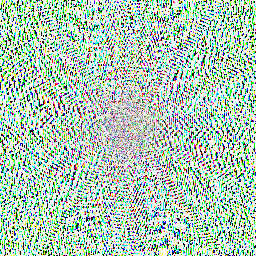
\includegraphics[width=0.25\linewidth]{Figures/2D_QDFTv1.png}
	}~
	\subfloat[\label{fig:2D_QDFTv2}]{
		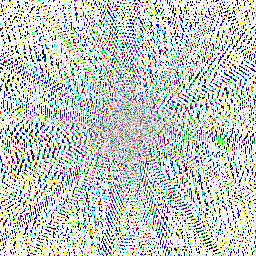
\includegraphics[width=0.25\linewidth]{Figures/2D_QDFTv2.png}
	}
	\caption{(a) 2D-QDFT da imagem na Fig. \ref{fig:dice} segundo (\ref{eq:2DQDFT}), com eixo $ \qmu = \frac{1}{\sqrt{3}}(\qi + \qj + \qk) $. (b) 2D-QDFT da mesma imagem, com mesmo eixo, segundo defini\c c\~ao alternativa em (\ref{eq:2DQDFTv2}).}
	\label{fig:QDFT}
\end{figure}

\section{Transformada Discreta de Fourier Quaterni\^onica Fracion\'aria}
\label{sec:FrQDFT}
%Incluir defini\c{c}\~ao da transformada, a qual sugiro que seja identificada pelo acr\^onimo FrQDFT (do ingl\^es \emph{fractional quat\'ernios discrete Fourier transform}), empregando o conte\'udo desenvolvido na se\c{c}\~ao anterior e abordar as principais propriedades.

O m\'etodo proposto para fracionariza\c c\~ao da QDFT explora o compartilhamento entre autovetores da DFT e da QDFT: uma vez que se disp\~oe de uma matriz ortogonal $ \mathbf{E} $ de autovetores da DFT, ela pode ser usada na diagonaliza\c c\~ao da matriz da QDFT e na sua subsequente fracionariza\c c\~ao. Por exemplo, a autodecomposi\c c\~ao da matriz $ \mathbf{F}_{\text{DFT}} $ da DFT permite obter a transformada discreta de Fourier fracion\'aria (FrDFT, \textit{fractional discrete Fourier transform}) a partir da potencia\c c\~ao n\~ao-inteira da matriz de autovalores,
\begin{equation}
\label{eq:FrDFT}
\mathbf{F}_{\text{DFT}}^a = \mathbf{E} \boldsymbol{\Lambda}^a \mathbf{E}^T,
\end{equation}
em que $ \boldsymbol{\Lambda}$ \'e a matriz diagonal contendo os autovalores da DFT.

Oliveira Neto e Lima \cite{de2017discrete} apontam que, para que a FrDFT em (\ref{eq:FrDFT}) aproxime numericamente a transformada fracion\'aria de Fourier cont\'inua, as componentes dos autovetores em $ \mathbf{E} $ precisam aproximar amostras das fun\c c\~oes Hermite-Gaussianas cont\'inuas. Em \cite{de2017discrete}, apresentam dois m\'etodos para gerar tal base ortogonal de autovetores, um dos quais (m\'etodo das matrizes geradoras) foi utilizado nos exemplos deste cap\'itulo.
%Se estes autovetores forem as colunas de uma matriz ortogonal $ \mathbf{E} $, com seus respectivos autovetores na matriz diagonal $ \mathbf{\Lambda} $, a fracionariza\c c\~ao da DFT \'e obtida ao elevar cada autovalor em $ \mathbf{\Lambda} $ a um par\^ametro n\~ao-inteiro $ a \in [0,1] $, e a matriz da DFT fracion\'aria \'e dada por

\begin{figure*}
	\centering
	\subfloat[\label{fig:dice}]{
		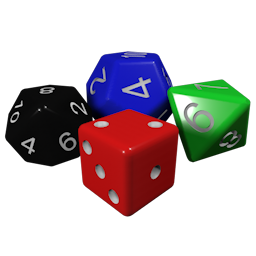
\includegraphics[width=0.25\linewidth]{Figures/dice_256x256.png}
	}~
	\subfloat[]{
		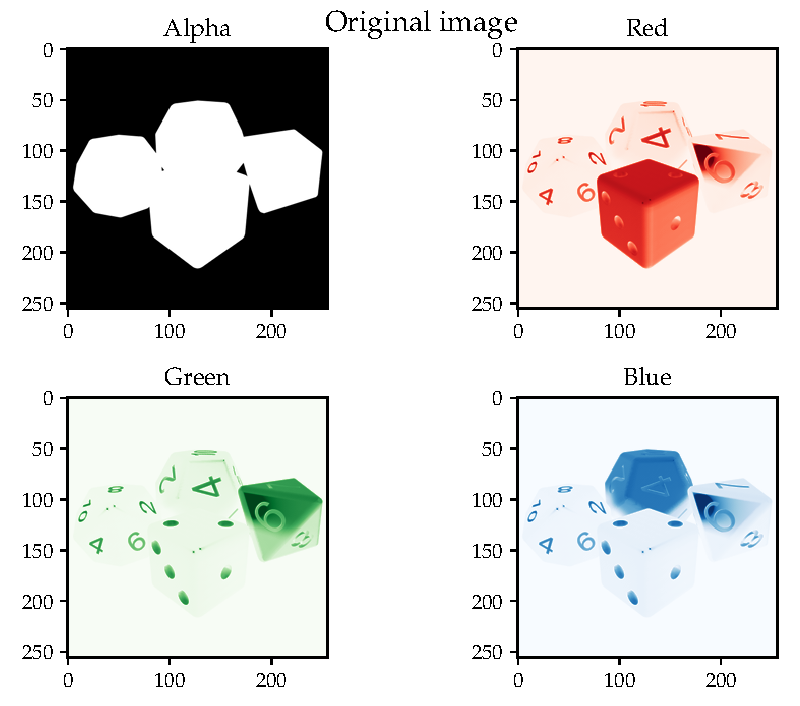
\includegraphics[width=0.35\linewidth]{Figures/dice_256x256_layers.pdf}
	}~
	\subfloat[]{
		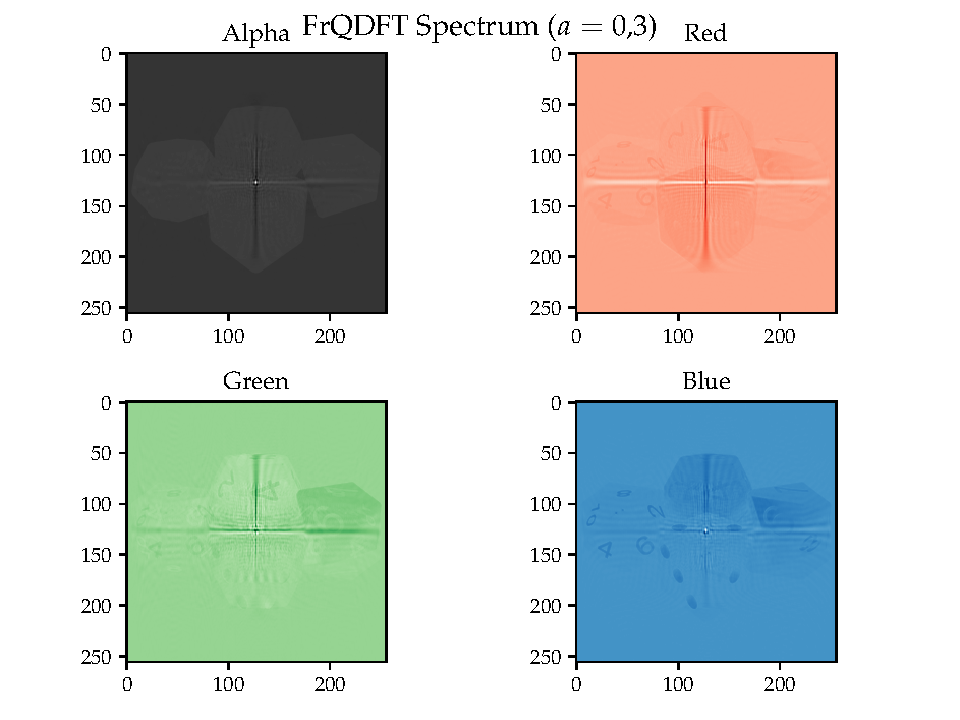
\includegraphics[width=0.35\linewidth]{Figures/dice_256x256_layers_frqdft.pdf}
	}~
	\caption{(a) Imagem de teste em formato PNG. (b) Visualiza\c c\~ao de cada uma das quatro camadas da imagem e (c) de seu espectro pela FrQDFT com $ \qmu = \frac{1}{\sqrt{3}}(\qi + \qj + \qk) $ e $ a=0{,}3 $.}
\end{figure*}

De posse de uma matriz ortogonal $ \mathbf{E} $, contendo autovetores do tipo Hermite-Gaussiano da DFT, o Teorema \ref{th:01} assegura que ela \'e tamb\'em uma base de autovetores da QDFT. Assim, a respectiva matriz $ \mathbf{F} $ tem sua autodecomposi\c c\~ao dada por
% -- e, em fun\c c\~ao do Teorema \ref{th:01}, tamb\'em da QDFT --, a matriz da transformada pode ser diagonalizada como
\begin{equation}
\label{eq:QDFTmtx}
\mathbf{F} = \mathbf{E} \boldsymbol{\Gamma} \mathbf{E}^T,
\end{equation}
%obtendo uma matriz $ \mathbf{E} $, cujas colunas s\~ao os autovetores do tipo Gauss-Hermite da transformada,
em que a matriz diagonal $ \boldsymbol{\Gamma} $ \'e obtida substituindo $ \qi $ por $ \qmu $ em $ \mathbf{\Lambda} $ (Tabela \ref{tab:01}). Desta forma, a vers\~ao fracion\'aria da QDFT, representada pelo acr\^onimo FrQDFT (do ingl\^es \emph{fractional quaternion discrete Fourier transform}), \'e obtida elevando cada autovalor em $ \boldsymbol{\Gamma} $ a um par\^ametro $ a \in \mathbb{R} $, chamado de ordem fracion\'aria, de modo que
\begin{equation}
\label{eq:QDFTmtxa2}
\text{FrQDFT}_a\{ \mathbf{v} \} \overset{\Delta}{=} \mathbf{F}^a \mathbf{v},
\end{equation}
%\ref{eq:QDFTmtx}
em que
\begin{equation}
\label{eq:QDFTmtxa}
\mathbf{F}^a = \mathbf{E} \boldsymbol{\Gamma}^a \mathbf{E}^T.
\end{equation}

A FrQDFT, tal como definida em (\ref{eq:QDFTmtxa2}) e (\ref{eq:QDFTmtxa}), guarda as propriedades cl\'assicas de uma transformada de Fourier fracion\'aria:
\begin{itemize}[noitemsep]
	\item \textit{Redu\c c\~ao \`a transformada quaterni\^onica ordin\'aria}: se $ a=1 $, ent\~ao a equa\c c\~ao de s\'intese da FrQDFT (\ref{eq:QDFTmtxa2}) reduz-se \`a equa\c c\~ao (\ref{eq:QDFT}), coincidindo com a QDFT. A prova \'e imediata.
	
	\item \textit{Redu\c c\~ao \`a Identidade}: se $ a=0 $, a FrQDFT reduz-se ao operador identidade.
	
	\begin{proof}
		Da ortogonalidade da matriz de autovetores $ \mathbf{E} $,
		\begin{equation}
		%\label{key}
		\mathbf{F}^0 = \mathbf{E} \boldsymbol{\Gamma}^0 \mathbf{E}^T = \mathbf{E} \mathbf{E}^T = \mathbb{I}.
		\end{equation}
	\end{proof}
	
	\item \textit{Aditividade de \'indices}: aplicar sucessivamente duas FrQDFT de par\^ametros $ a $ e $ b $, respectivamente, equivale a uma FrQDFT de par\^ametro $ a+b $. Ou seja, $ \mathbf{F}^a \mathbf{F}^b = \mathbf{F}^{a+b} $.
	
	\begin{proof}
		\begin{equation}
		%\label{key}
		\begin{aligned}
		\mathbf{F}^a \mathbf{F}^b &= \mathbf{E} \boldsymbol{\Gamma}^a \mathbf{E}^T
		\mathbf{E} \boldsymbol{\Gamma}^b \mathbf{E}^T \\
		&= \mathbf{E} \boldsymbol{\Gamma}^a \boldsymbol{\Gamma}^b \mathbf{E}^T,
		\end{aligned}
		\end{equation}
		mas, sendo $ \boldsymbol{\Gamma} $ uma matriz diagonal, $ \boldsymbol{\Gamma}^a \boldsymbol{\Gamma}^b =
		\boldsymbol{\Gamma}^{a+b} $, logo
		%mas, sendo $ \gamma_n $ a $ n $-\'esima entrada na diagonal principal de $ \boldsymbol{\Gamma} $,
		%Como $ \boldsymbol{\Gamma} $ \'e uma matriz diagonal $ \boldsymbol{\Gamma} = \text{diag} (\gamma_0, \gamma_1, \dots, \gamma_{N-1}) $,
		%\begin{equation}
		%%\label{key}
		%\{ \boldsymbol{\Gamma}^a \boldsymbol{\Gamma}^b \}_{n,n} =
		%\gamma^a_n \gamma^b_n = (\gamma_n)^{a+b} =
		%\{ \boldsymbol{\Gamma}^{a+b} \}_{n,n},
		%\end{equation}
		\begin{equation}
		%\label{key}
		\mathbf{F}^a \mathbf{F}^b = \mathbf{E} \boldsymbol{\Gamma}^a \boldsymbol{\Gamma}^b \mathbf{E}^T = \mathbf{E} \boldsymbol{\Gamma}^{a+b} \mathbf{E}^T =
		\mathbf{F}^{a+b}.
		\end{equation}
	\end{proof}
	
	\item \textit{Matriz unit\'aria}: a matriz $ \mathbf{F}^a $ \'e unit\'aria, i.~e.
	\begin{equation}
	%\label{key}
	\mathbf{F}^a (\mathbf{F}^a)^H = \mathbb{I},
	\end{equation}
	em que $ \mathbb{I} $ \'e a matriz identidade e $ (\cdot)^H $ denota o conjugado\footnote{A opera\c c\~ao de conjuga\c c\~ao \'e tomada no sentido quaterni\^onico, i.~e. se $ q = a + b\qi + c\qj + d\qk = r \exp (\qmu \theta) $, ent\~ao seu conjugado \'e $ \bar{q} = a - b\qi - c\qj - d\qk = r \exp (-\qmu \theta) $} transposto de uma matriz.
	
	\begin{proof}
		Uma vez que todos os autovalores $ \gamma_n $ da FrQDFT s\~ao ra\'izes quartas da unidade no plano 1-$\qmu $ (i.~e. $ \gamma_n = \pm 1, \pm \qmu $ e, portanto, t\^em m\'odulo unit\'ario), ent\~ao podem ser escritos na forma $ \gamma_n = \exp \qmu \theta $ (em que $ \theta = 0, \pm \frac{\pi}{2}, \pi $). Assim,
		\begin{equation}
		%\label{key}
		\overline{\gamma^a_n} = \gamma_n = \exp (-a \qmu \theta) = \gamma^{-a}_n,
		\end{equation}
		ou seja,
		\begin{equation}
		\label{eq:24}
		(\boldsymbol{\Gamma}^a)^H = \boldsymbol{\Gamma}^{-a}.
		\end{equation}
		
		De (\ref{eq:24}) e (\ref{eq:QDFTmtxa}),
		\begin{equation}
		%\label{key}
		\begin{aligned}
		%\label{key}
		(\mathbf{F}^a)^H &=  \left((\mathbf{E} \boldsymbol{\Gamma}^a) \mathbf{E}^T \right)^H \\
		&=  \mathbf{E} \left(\mathbf{E} \boldsymbol{\Gamma}^a  \right)^H =
		\mathbf{E} (\boldsymbol{\Gamma}^{a})^H \mathbf{E}^T \\
		&= \mathbf{E} \boldsymbol{\Gamma}^{-a} \mathbf{E}^T = \mathbf{F}^{-a},
		\end{aligned}
		\end{equation}
		e, pela aditividade de \'indices e redu\c c\~ao \`a identidade,
		\begin{equation}
		%\label{key}
		\begin{aligned}
		%\label{key}
		\mathbf{F}^a (\mathbf{F}^a)^H = \mathbf{F}^a \mathbf{F}^{-a} = \mathbf{F}^0= \mathbb{I}.
		\end{aligned}
		\end{equation}
	\end{proof}
\end{itemize}


\section{A FrQDFT Multiparam\'etrica com Aplica\c{c}\~ao em Cifragem de Imagens Coloridas}
\label{sec:multi}
%Indicar que se trata de uma aplica\c{c}\~ao ilustrativa da FrQDFT, motivada pelo fato de se empregar, comumente, a transformada fracion\'aria de Fourier para cifrar imagens monocrom\'aticas. Sugiro que, nos experimentos, sejam usadas imagens no formato .png, que, se incluirmos a camada de transpar\^encia, possuem quatro camadas que podem ser mapeadas justamente nos quatro coeficientes quaterni\^onicos. Posso passar mais detalhes sobre isso depois.
\'E frequente a utiliza\c c\~ao de transformadas fracion\'arias em cifragem de imagens, tanto monocrom\'aticas \cite{tao2010image} como coloridas \cite{kang2018reality, kang2018color}. A associa\c c\~ao da chave do algoritmo de cifragem \`a ordem da transformada, juntamente com o uso de m\'ultiplas transforma\c c\~oes, ou de transformadas multiparam\'etricas, permite criar sistemas com espa\c co de chaves suficientemente grandes e alta sensibilidade a erros na chave. Neste contexto, esta se\c c\~ao apresenta uma aplica\c c\~ao ilustrativa da FrQDFT, na qual pretende-se definir uma vers\~ao multiparam\'etrica da transformada e utiliz\'a-la num esquema de cifragem de imagens PNG, processando-as de forma hol\'istica a cada etapa do algoritmo.

%Kang \textit{et al.}  seguiram um caminho semelhante e aplicaram uma transformada fracion\'aria angular e uma vers\~ao fracion\'aria da transformada de Hartley como parte de seu algoritmo de cifragem de imagens coloridas. Chen \cite{chen2018quaternion} utilizou uma transformada aleat\'oria fracion\'aria quaterni\^onica para realizar marcas-d'\'agua adaptativas em imagens coloridas.
%O processamento hol\'istico de imagens coloridas foi sugerido por Ell e Sangwine \cite{ell2007hypercomplex}, quando propuseram atribuir a cada componente da parte vetorial de um quat\'ernio puro um canal de cor do pixel de uma imagem colorida, de modo que a an\'alise espectral poderia ser realizada atrav\'es da QFT bidimensional. Chen \cite{chen2018quaternion} utilizou uma transformada aleat\'oria fracion\'aria quaterni\^onica para realizar marcas-d'\'agua adaptativas em imagens coloridas.
A defini\c c\~ao da FrQDFT multiparam\'etrica, denotada por MFrQDFT, consiste em empregar ordens fracion\'arias di\-fe\-ren\-tes para cada autovalor em $ \boldsymbol{\Gamma} $, armazenadas no vetor $ \mathbf{a} = [a_0, a_1, \dots, $ $ a_{N-1}] $. A aplica\c c\~ao da transformada ao vetor-coluna $ \mathbf{v} $ resulta, portanto, em
\begin{equation}
\label{eq:MFrQDFT}
\text{MFrQDFT}\{ \mathbf{v} \} = \mathbf{E} \boldsymbol{\Gamma}\mathbf{^a} \mathbf{E}^T \mathbf{v} = \mathbf{F^a} \mathbf{v}.
\end{equation}

As express\~oes $ \boldsymbol{\Gamma}\mathbf{^a} $ e $ \mathbf{F^a} $ em (\ref{eq:MFrQDFT}) s\~ao um abuso de nota\c c\~ao. Deve-se compreender $ \boldsymbol{\Gamma}\mathbf{^a} $ como a matriz diagonal obtida ap\'os elevar a $ n $-\'esima entrada da diagonal de $ \boldsymbol{\Gamma} $ ao $ n $-\'esimo elemento do vetor $ \mathbf{a} $. Quanto a $ \mathbf{F^a} $, trata-se do s\'imbolo indicando a matriz $ \mathbf{E} \boldsymbol{\Gamma}\mathbf{^a} \mathbf{E}^T $. Assim como feito na Subse\c c\~ao \ref{subsec:2D_QDFT}, a MFrQDFT bidimensional aplicada a uma matriz quaterni\^onica $ \mathbf{X} $, e.~g. representando uma imagem PNG, \'e definida como
\begin{equation}
\label{eq:2DMFrQDFT}
\text{2D-MFrQDFT}\{\mathbf{X} \} \overset{\Delta}{=} \mathbf{F^a} \mathbf{X} \mathbf{F^a}^T,
\end{equation}
com transformada inversa obtida das propriedades listadas na Se\c c\~ao \ref{sec:FrQDFT},
\begin{equation}
\label{eq:2DMFrQDFTinv}
\text{2D-MFrQDFT}^{-1}\{ \mathbf{\widehat{X}} \} = (\mathbf{F^a}^H) \mathbf{\widehat{X}} (\overline{\mathbf{F^a}}).
\end{equation}

\begin{figure*}
	\centering
	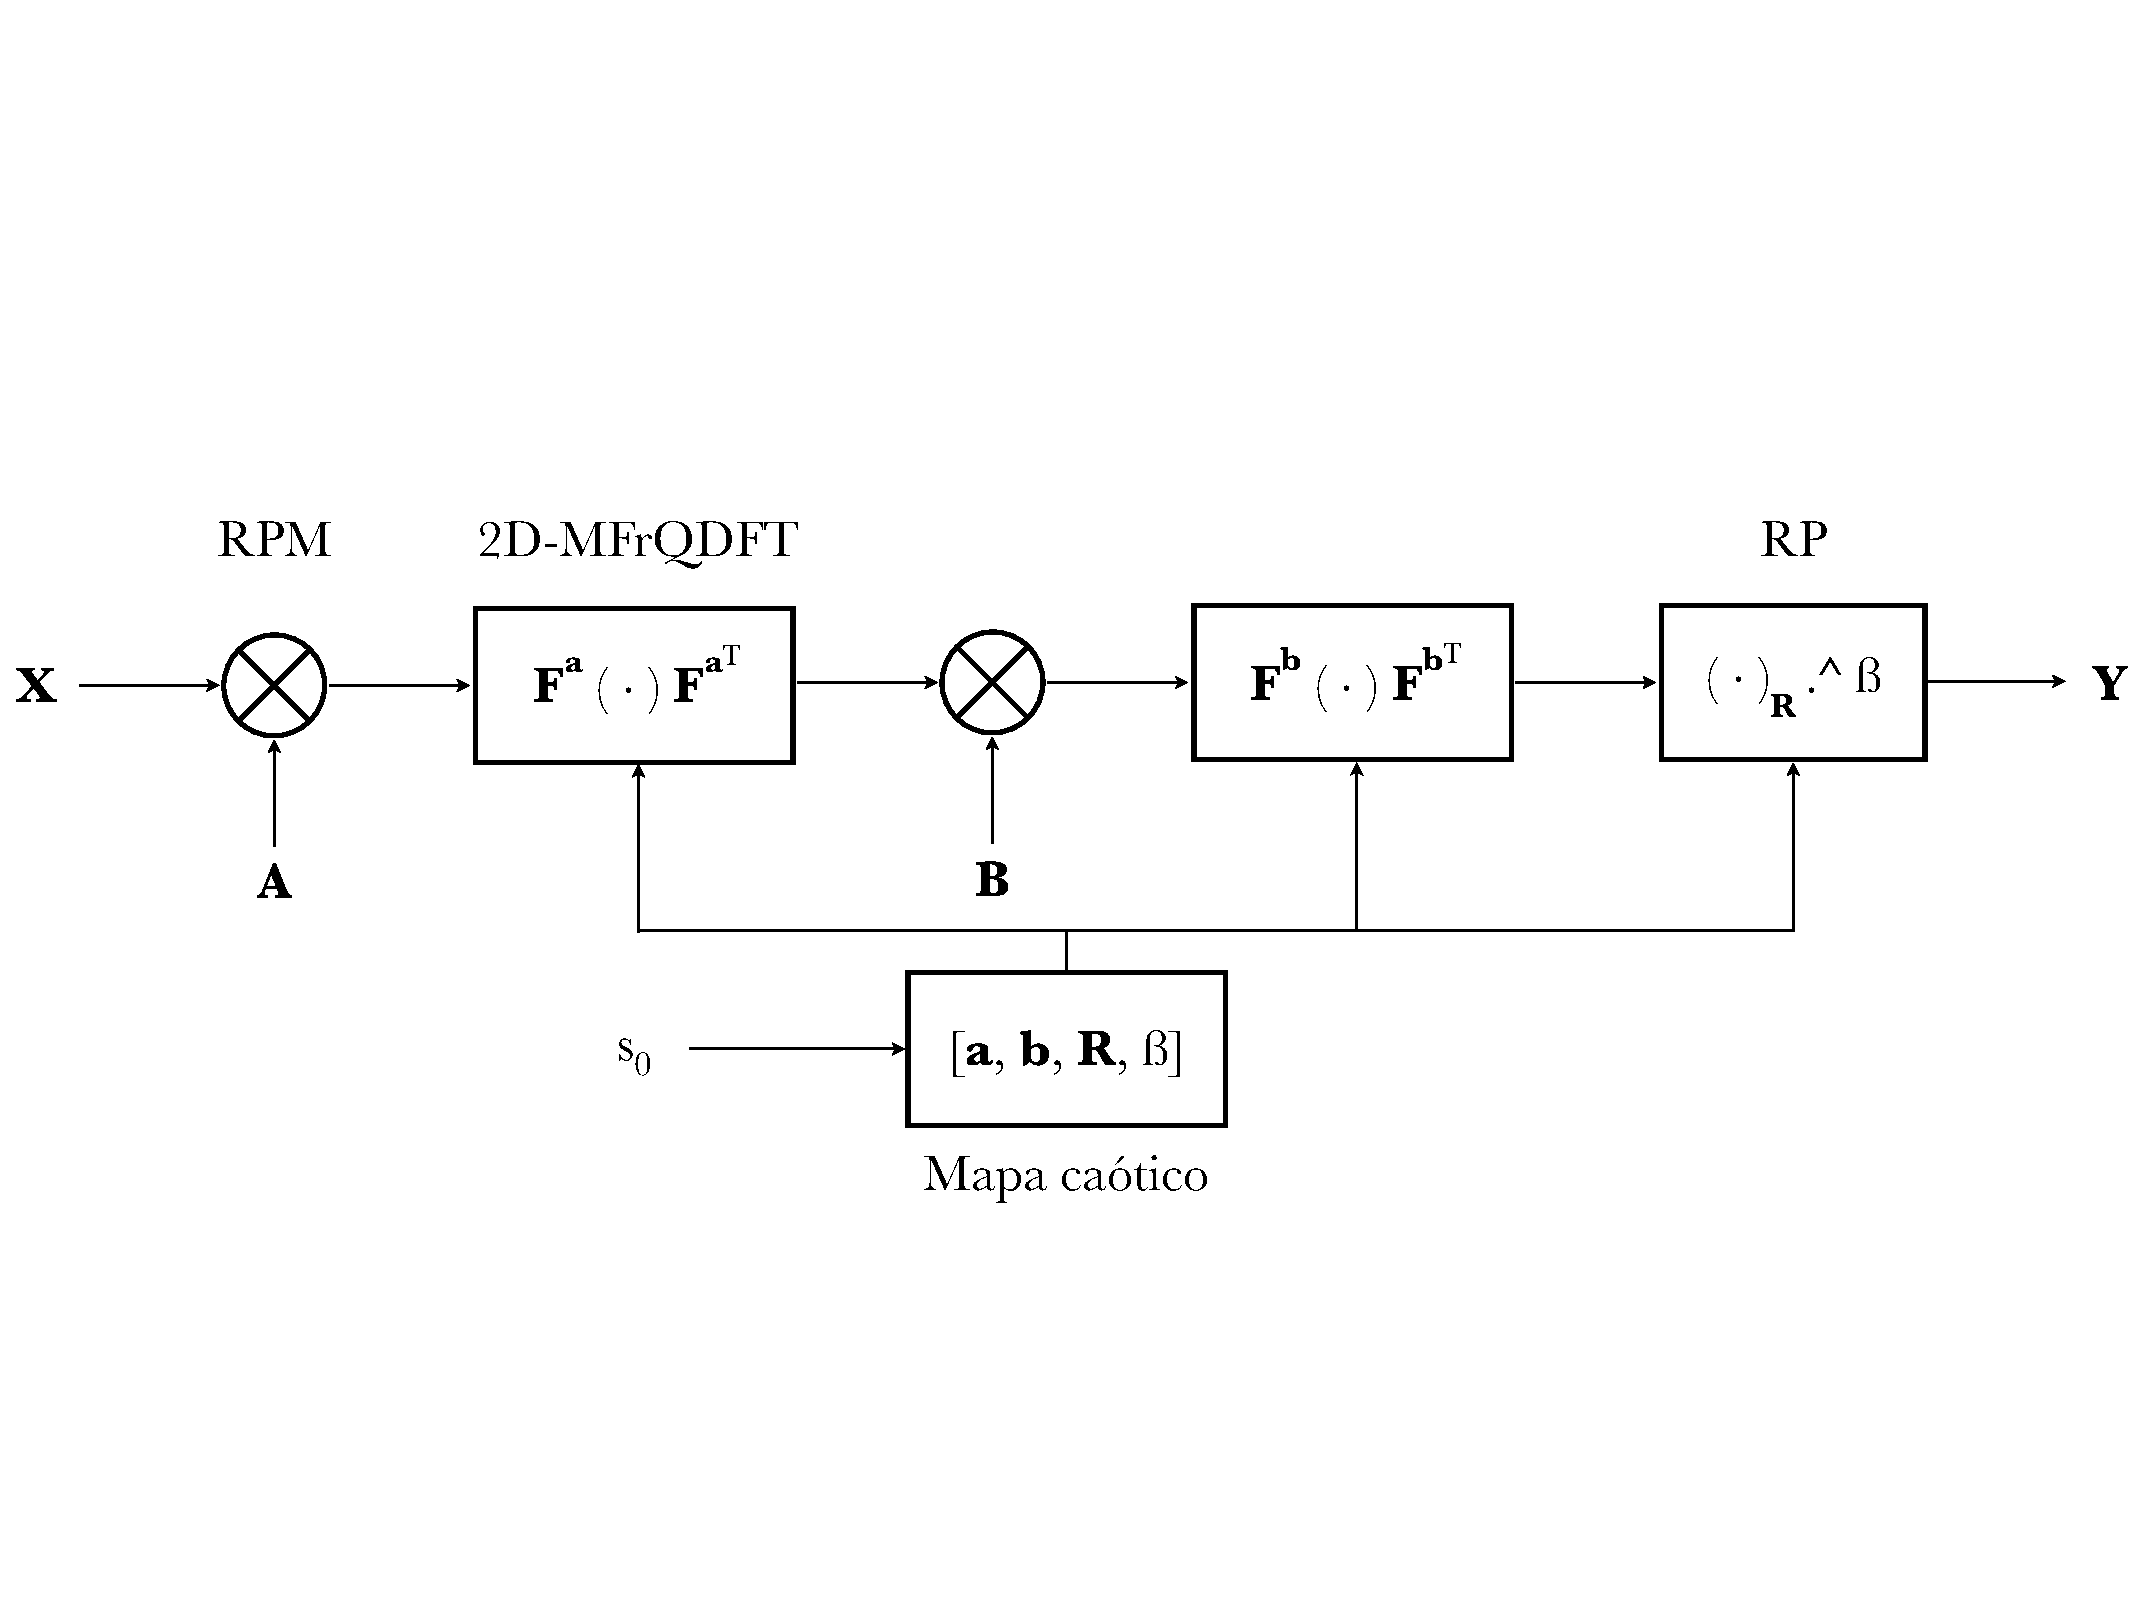
\includegraphics[width=0.9\linewidth]{Figures/esquema_PT.pdf}
	\caption{Esquema de cifragem proposto, explorando a MFrQDFT.}
	\label{fig:cifragem}
\end{figure*}

\begin{figure*}
	\centering
	\subfloat[\label{fig:ciphered01}]{
		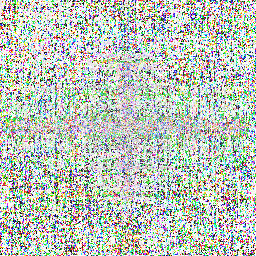
\includegraphics[width=0.3\linewidth]{Figures/sage_Encrypted_image.png}
	}~
	\subfloat[\label{fig:ciphered02}]{
		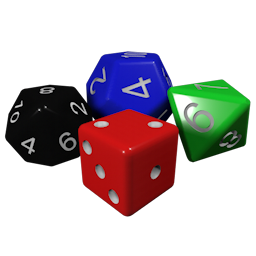
\includegraphics[width=0.35\linewidth]{Figures/Decrypted_image_error_0.png}
	}~
	\subfloat[\label{fig:ciphered03}]{
		
\includegraphics[width=0.3\linewidth]{Figures/sage_Decrypted_image_error_minus1dot6.png}
	}~
	\caption{(a) Imagem cifrada. (b) Imagem decifrada com a chave $ s_0 $ correta. (c) Imagem decifrada com a chave errada $ \widetilde{s_0} = s_0 + \epsilon $, com $ \epsilon = -1{,}6 \cdot 10^{-80} $.}
\end{figure*}

\subsection{Esquema de cifragem utilizando a MPFrQDFT}

Optou-se por implementar um algoritmo de cifragem de imagens coloridas (possivelmente com camada de opacidade) misturando modula\c c\~ao de fase aleat\'oria (RPM, \textit{random-phase modulation}, tamb\'em chamada de m\'ascara de fase em \cite{chen2018multiple} e \cite{singh2008optical}) e transformada multiparam\'etrica. Como sugerido por \cite{hsue2018enhancing}, um bloco n\~ao-linear de potencia\c c\~ao aleat\'oria \'e tamb\'em utilizado. A Fig. \ref{fig:cifragem} ilustra os componentes do sistema.

A imagem a ser cifrada \'e, inicialmente, convertida em uma matriz quaterni\^onica $ \mathbf{X} $, ao que seguem duas rodadas de RPM $ + $ 2D-MFrQDFT. A modula\c c\~ao de fase aleat\'oria consiste na multiplica\c c\~ao elemento-a-elemento por uma matriz de quat\'ernios unit\'arios, gerados aleatoriamente. Este \'e o papel das matrizes $ \mathbf{A} $ e $ \mathbf{B} $ na Fig. \ref{fig:cifragem}. A invers\~ao de um bloco de RPM, na decifragem, \'e feita simplesmente utilizando o \textit{conjugado} da matriz de quat\'ernios unit\'arios.

Por fim, o esquema prev\^e um bloco n\~ao-linear de potencia\c c\~ao aleat\'oria (RP, \textit{random power}). Sua fun\c c\~ao \'e elevar \textit{algumas} entradas da matriz quaterni\^onica a um expoente aleat\'orio $ \beta \in \ ]0,1[$. As entradas s\~ao selecionadas por uma matriz bin\'aria $ \mathbf{R} $, de forma que a resposta do bloco de RP a uma certa matriz de entrada $ \mathbf{M} $ \'e
\begin{equation}
%\label{key}
\text{RP}(\mathbf{M})_{i,j} =
\begin{cases}
(\mathbf{M}_{i,j})^\beta & \text{se } \mathbf{R}_{i,j} = 1, \\
\mathbf{M}_{i,j} & \text{se } \mathbf{R}_{i,j} = 0.
\end{cases}
\end{equation}
Na decifragem, utiliza-se um bloco RP com a mesma matriz $ \mathbf{R} $ e um expoente $ \beta^{-1} $.

Utilizou-se um mapa ca\'otico para produzir uma sequ\^encia pseudo-aleat\'oria $ \mathbf{s} $ de n\'umeros entre 0 e 1, a partir da qual foram extra\'idos os vetores de par\^ametros fracion\'arios das duas 2D-MFrQDFT, o expoente $ \beta $ e a matriz $ \mathbf{R} $\footnote{Para cada entrada $ \mathbf{R}_{i,j} $, tomou-se um elemento $ s_k $ de $ \mathbf{s} $ e fez-se $ \mathbf{R}_{i,j} = 1 $ se $ s_k > 0{,}5 $, $ \mathbf{R}_{i,j} = 0 $ caso contr\'ario.}. Assim, para processamento de uma imagem de tamanho $ 256 \times 256 $ pixels, gera-se uma sequ\^encia de comprimento  $ 256 + 256 + 256^2 + 1  $. A chave secreta do esquema de cifragem consiste apenas na semente $ s_0 $ do mapa ca\'otico, uma vari\'avel em ponto flutuante. O espa\c co de chaves, portanto, fica determinado pelo menor desvio $ \epsilon $ de $ s_0 $ tal que a decifragem utilizando $ \widetilde{s_0} = s_0 \pm \epsilon $ produz uma imagem sem qualquer resqu\'icio da informa\c c\~ao original.

A dimens\~ao do espa\c co de chaves, denotada aqui por $ [K] $, \'e a raz\~ao entre o comprimento do intervalo de valores para $ s_0 $ e o do intervalo de valores diferentes da chave correta, tais que ainda \'e poss\'ivel reconstru\c c\~ao parcial da imagem, i.e. $ [s_0 - \epsilon, s_0 + \epsilon] $. Uma vez que $ s_0 \in \ ]0,1[ $, 
\begin{equation}
%\label{key}
[K] = \frac{1 - 0}{s_0 + \epsilon - (s_0 - \epsilon)} = \frac{1}{2 \epsilon}.
\end{equation}

Para teste do esquema de cifragem, o mapa ca\'otico es\-co\-lhi\-do foi o mapa aleat\'orio de tenda (\textit{tent map}) \cite{singh2008optical}, definido pela recurs\~ao
\begin{equation}
%\label{key}
s_{n+1} =
\begin{cases}
\gamma s_n & \text{se } 0 \leq s_0 < 0{,}5, \\
\gamma(1 - s_n) & \text{se } 0{,}5 \leq s_0 \leq 1.
\end{cases}
\end{equation}
com $ \gamma \in \ ]0,2] $.

Utilizou-se $ s_0 = 0{,}3 $ e $ \gamma = 1{,}8 $ como par\^ametros do mapa de tenda. A imagem na Fig. \ref{fig:dice} foi cifrada segundo o esquema proposto, gerando como resultado a Fig. \ref{fig:ciphered01}.

Para avaliar a dimens\~ao do espa\c co de chaves, foi realizada a decifragem com chaves $ \widetilde{s_0} = s_0 \pm \epsilon $ para diferentes valores de $ \epsilon \in [-10 \times 10^{-80}; 10 \times 10^{-80}]$, utilizando a aritm\'etica de m\'ultipla precis\~ao provida pela classe \textit{RealField} do software SageMath. Ao fim de cada decifragem, foi obtido o MSE com rela\c c\~ao \`a imagem original e os valores s\~ao mostrados na Fig. \ref{fig:MSE}. O gr\'afico do MSE n\~ao varia de forma suave porque, a cada mudan\c ca pequena (maior que -- ou da ordem de -- $ 10^{-80} $) na semente $ s_0 $, toda a sequ\^encia $ \mathbf{s} $ altera-se de maneira aparentemente ca\'otica. O menor MSE calculado (com $ \epsilon \neq 0 $) foi 39dB, com $ \epsilon = -1{,}6 \times 10^{-80} $.

As Fig. \ref{fig:ciphered02} e \ref{fig:ciphered02} trazem os resultados da decifragem com $ \epsilon = 0 $ e $ \epsilon = -1{,}6 \times 10^{-80} $, ilustrando que mesmo o valor do erro n\~ao-nulo que produziu o menor MSE, ainda assim produziu uma imagem ruidosa e sem informa\c c\~ao. O menor valor de erro utilizado foi $ 0{,}83 \times 10^{-80} $, do que se pode concluir que o espa\c co de chaves tem dimens\~ao, no m\'inimo, igual a
\begin{equation}
%\label{key}
[K] = \frac{1}{2 \times 0{,}83 \times 10^{-80}} \approx 6{,}0 \times 10^{79},
\end{equation}
o que significa que cada chave deve ter comprimento de
\begin{equation}
%\label{key}
\lceil 79 \log_2 10 \rceil = 263\text{ bits},
\end{equation}
maior do que os 256 bits que, segundo relat\'orios como o ECRYPT \cite{smart2018algorithms}, \'e um tamanho de chaves apropriado para manter sistemas de cifra sim\'etrica em uso por um per\'iodo estimado de 30 a 50 anos.

%considerando os testes e orienta\c c\~oes de relat\'orios como o {\color{red}ECRYPT II da \textit{European Network of Excellence in Cryptology II}, de 2012} \cite{smart2018algorithms}, que indicou .

%A Fig. \ref{fig:RPM} ilustra a oculta\c c\~ao gradual de informa\c c\~ao visual, ao menos nos pixels n\~ao-nulos, ap\'os cada itera\c c\~ao do bloco de RPM. A cada itera\c c\~ao, uma matriz aleat\'oria diferente \'e usada.

\begin{figure}
	\centering
	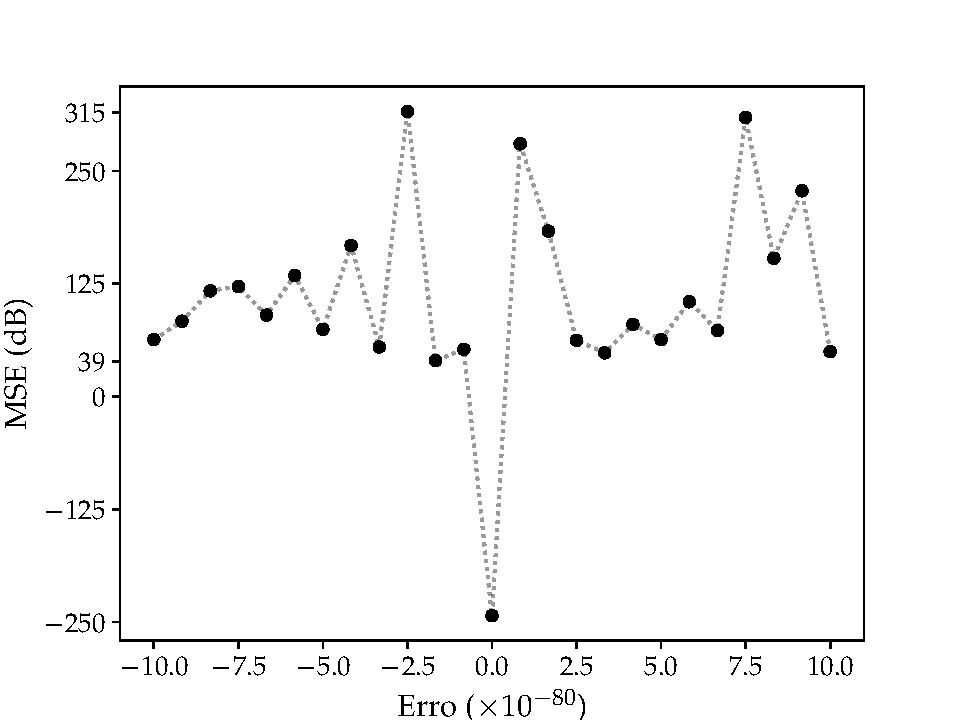
\includegraphics[width=0.7\linewidth]{Figures/MSEdb_FrQDFT_PT.pdf}
	\caption{Erro m\'edio quadr\'atico, em dB, da imagem decifrada, em fun\c c\~ao do erro $ \epsilon $ imposto \`a chave.}
	\label{fig:MSE}
\end{figure}

\section{Conclus\~oes}
\label{sec:conclusao}
Neste cap\'itulo foi investigada a autoestrutura da transformada discreta de Fourier quaterni\^onica. Apesar da autodecomposi\c c\~ao de matrizes quaterni\^onicas ser um problema permeado de detalhes e considera\c c\~oes --- o que \'e objeto de pesquisa em curso, comentado no ca\'itulo \ref{ch:QGSP} ---, o caso da QDFT foi solucionado ap\'os a demonstra\c c\~ao do com\-par\-ti\-lha\-men\-to de autovetores entre esta transformada e a DFT. A partir de m\'etodos da literatura para garantir a constru\c c\~ao desta base de autovetores, uma vers\~ao fracion\'aria da QDFT foi proposta, apresentando propriedades semelhantes \`aquelas da FrDFT. Explorando a natureza quadridimensional dos quat\'ernios, a aplica\c c\~ao da FrQDFT foi ilustrada atrav\'es de um esquema de cifragem hol\'istica das quatro camadas de uma imagem colorida com camada de opacidade, o que incluiu a defini\c c\~ao de uma vers\~ao multiparam\'etrica da transformada.


\chapter{Quaternion graph signal processing}
\label{ch:QGSP}

Numerous studies in the last decade have contributed to establish graph signal processing as a fruitful and promising field of research. Sharing the main aim of generalizing principles and techniques of classical signal processing to the context of network-based signal domain~\cite{ortega2018graph}, two main approaches have risen through the recent years and they constitute the root of GSP. The first one --- that presented in section \ref{sec:GSPintro} --- stems from algebraic signal processing, using the weighted adjacency matrix and elementary block. This approach deals with signals defined on both directed and undirected graphs, with both real- and complex-valued edge weights~\cite{sandryhaila2014big}. The second one is based on spectral graph theory and focuses only on signals defined on undirected graphs with real-valued edge weights, using the graph Laplacian matrix to build the signal space~\cite{shuman2013emerging}.

Recent formulations of GSP have unified the two by stating that, regardless of the graph matrix at hand (Laplacian, adjacency, and others \cite{chen2018shift, dees2019unitary}), all GSP tools emerge from the choice of unit graph shift operator. Similarly to classical DSP, the shift operator generates the eigenbasis of linear and shift invariant filters ("linear and time invariant", in the discrete-time domain).
As shown in section \ref{sec:GSPintro}, the eigendecomposition of this operator plays a central role in GSP.

\begin{figure}
	\centering
	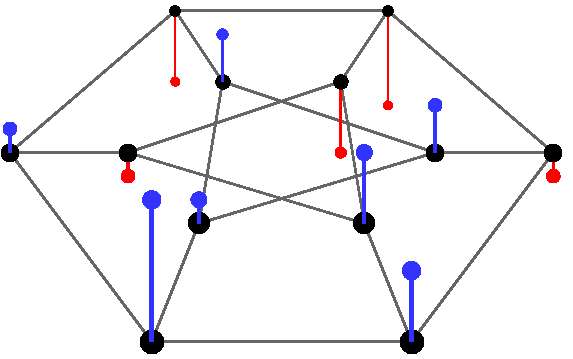
\includegraphics[width=0.3\linewidth]{Figures/signal_duher_graph_2.pdf}
	\caption{Example of graph signal. The graph edges capture similarity or interdependency relationship between samples. What new possibilities are created when the edges carry quaternion weights? Source: the author.}
	\label{fig:duher}
\end{figure}

A depender do problema abordado com GSP, o grafo utilizado pode ser direcionado ou n\~ao-direcionado, com arestas de pesos reais ou complexos. A explora\c c\~ao de diferentes \'algebras abre possibilidades para novas ferramentas e interpreta\c c\~oes, como ocorreu com a modelagem de sinais el\'etricos utilizando fun\c c\~oes a valores complexos. Os engenheiros eletricistas puderam usufruir de vari\'aveis que, carregando duas informa\c c\~oes (amplitude e fase), mostraram-se mais apropriadas \`a visualiza\c c\~ao e \`a manipula\c c\~ao de sinais harm\^onicos do que se apenas fun\c c\~oes reais fossem usadas. Este foi o racioc\'inio de Ortoloni e Uncini \cite{ortolani2016quaternion}, ao propor o estudo de processamento de sinais de tempo discreto com valores \emph{quaterni\^onicos}.

%mostrou que a  utilizando filtros quaterni\^onicos adaptativos, juntamente com o algoritmo de m\'inimos quadrados sobre quat\'ernios, obt\'em uma taxa de converg\^encia no dom\'inio da frequ\^encia maior do que no dom\'inio do tempo.

Assim como Jiang et al. \cite{jiang2013frequency} beneficiaram-se ao modelar o problema de predi\c c\~ao de perfis de vento (sinais tridimensionais contendo a dire\c c\~ao do vento em cada ponto do espa\c co) utilizando a vers\~ao quaterni\^onica de filtros adaptativos LMS, ou Flamant et al. \cite{flamant2018complete} criaram um arcabou\c co para an\'alise tempo-frequ\^encia de sinais bivariados usando quat\'ernios, a hip\'otese deste projeto de tese \'e que o estudo sobre GSP com valores quaterni\^onicos pode ter implica\c c\~oes te\'oricas e pr\'aticas de valor. O que poder\'iamos chamar de QGSP (\emph{quaternion graph signal processing}) consiste em lidar com as consequ\^encias de criar um \emph{grafo com pesos quaterni\^onicos}.

Poss\'iveis aplica\c c\~oes de QGSP devem surgir em cen\'arios em que n\~ao apenas o sinal sobre o grafo \'e tri- ou quadrimensional, mas tamb\'em a rela\c c\~ao entre as amostras. Por exemplo, um sinal que indique orienta\c c\~oes no espa\c co (dire\c c\~oes do vento, ou posi\c c\~oes de um objeto gr\'afico), modelado atrav\'es de quat\'ernios puros. Em processamento de sinais quaterni\^onicos, o \emph{sinal} \'e composto de quat\'ernios, mas \emph{n\~ao o dom\'inio}, como em QGSP.

%\red{O artigo \emph{GRAPH-BASED RGB-D IMAGE SEGMENTATION USING COLOR-DIRECTIONAL-REGION MERGING} seria uma poss\'ivel aplica\c c\~ao?

%Ou quem sabe um graph signal contendo posi\c c\~oes no espa\c co 3D, com arestas contendo os quat\'ernios que causam rota\c c\~ao no espa\c co?}

%\section{Fundamentos de GSP}
%\label{sec:GSP}

\section{Da teoria de matrizes quaterni\^onicas}

Na an\'alise da autoestrutura e subsequente fracionariza\c c\~ao da matriz da QDFT, foi tomada como atalho a autodecomposi\c c\~ao da DFT e o compartilhamento de autovetores entre as transformadas. Para elaborar resultados de QGSP, no entanto, \'e preciso mergulhar nas propriedades gerais de matrizes sobre quat\'ernios. A decomposi\c c\~ao simpl\'etica, apresentada em (\ref{eq:decomposicao}), desempenha um papel importante no estudo de matrizes quaterni\^onicas, particularmente por ajudar a definir a \emph{matriz complexa adjunta}.

\begin{definition}[Matriz complexa adjunta \cite{zhang1997quaternions}]
Dada a matriz $ \mathbf{A} \in \mathbb{H}^{n \times n} $, com decomposi\c c\~ao simpl\'etica $ \mathbf{A}_1 + \mathbf{A}_2 \qj$, $ \mathbf{A}_1,\mathbf{A}_2 \in \mathbb{C}^{n \times n} $, sua matriz complexa adjunta \'e dada por
\begin{equation}
\rchi_{A} \overset{\Delta}{=}
\begin{pmatrix}
\mathbf{A}_1 & \mathbf{A}_2\\ 
- \overline{\mathbf{A}}_2 & \overline{\mathbf{A}}_1
\end{pmatrix}.
\end{equation}
\end{definition}

Nos teoremas seguintes, Zhang traz resultados que desempenhar\~ao um importante papel no desenvolvimento de QGSP.

\begin{theorem}[Parte do Teorema 4.2 em
\cite{zhang1997quaternions}
]
\label{th:equiv01}
Dada a matriz $ \mathbf{A} \in \mathbb{H}^{n \times n} $, as seguintes afirma\c c\~oes s\~ao equivalentes:

\begin{itemize}[noitemsep]
\item $ \rchi_{AB} = \rchi_{A} \rchi_{B} $,
\item $ \rchi_{A^{-1}} = \rchi_{A}^{-1}$, se $ \mathbf{A}^{-1} $ existir,
\item $ \rchi_{A}$ \'e unit\'aria, hermitiana ou normal se e somente se $ \mathbf{A} $ tamb\'em o for.
\end{itemize}

\end{theorem}

\begin{theorem}[Parte do Teorema 4.3 em
\cite{zhang1997quaternions}
]
\label{th:equiv02}
Dada a matriz $ \mathbf{A} \in \mathbb{H}^{n \times n} $, as seguintes afirma\c c\~oes s\~ao equivalentes:

\begin{itemize}[noitemsep]
\item $\mathbf{A}$ \'e invers\'ivel.
\item $\mathrm{det}(\rchi_A) \neq 0$, i.e. $\rchi_{A}$ \'e invers\'ivel.
\end{itemize}

\end{theorem}


% Em \cite[Teoremas 4.2 e 4.3]{zhang1997quaternions}, Zhang traz alguns resultados interessantes da literatura a respeito de $ X_A $, dos quais cabe mencionar:
% \begin{itemize}[noitemsep]
% \item $ \rchi_{AB} = \rchi_{A} \rchi_{B} $,
% \item $ \rchi_{A^{-1}} = \rchi_{A}^{-1}$, se $ \mathbf{A}^{-1} $ existir,
% \item $ \rchi_{A}$ \'e unit\'aria, hermitiana ou normal se e somente se $ \mathbf{A} $ tamb\'em o for.
% \end{itemize}

A matriz complexa adjunta serve como uma representa\c c\~ao complexa da matriz quaterni\^onica e, diferente de outras representa\c c\~oes matriciais em $ \mathbb{C} $ ou $ \mathbb{R} $, esta permite estabelecer um v\'inculo entre o espectro de $ \rchi_{A} $ e o de $ \mathbf{A} $, como ser\'a discutido adiante.

\subsection{Autovalores}

Uma vez que a multiplica\c c\~ao sobre os quat\'ernios n\~ao \'e comutativa, faz-se necess\'ario distinguir os \emph{autovalores \`a esquerda} e os \emph{autovalores \`a direita} de uma matriz $ \mathbf{A} \in \mathbb{H}^{n \times n} $,
\begin{align*}
\mathbf{A} \mathbf{v} &= \mathbf{v} \lambda, \tag{autovalor \`a direita} \\
\mathbf{A} \mathbf{v} &= \lambda \mathbf{v}.  \tag{autovalor \`a esquerda}
\end{align*}

Uma vez que o problema dos autovalores \`a direita foi mais compreendido do que daqueles \`a esquerda, e possui mais resultados \cite[Cap. 5]{zhang1997quaternions}, restringiremos a an\'alise aos autovalores \`a direita. Quando n\~ao for mencionado, estes ser\~ao chamados apenas de \emph{autovalores} da matriz quaterni\^onica.

\'E importante mencionar que uma matriz quaterni\^onica possui um n\'umero \emph{finito} de autovalores se, e somente se, s\~ao todos reais. Do contr\'ario, cada autovalor pertence a uma classe de similaridade, segundo a transforma\c c\~ao $ \lambda_1 = q^{-1} \lambda_2 q $, contendo \emph{infinitos} outros quat\'ernios que tamb\'em s\~ao autovalores da matriz. Seja, por exemplo, o autovalor $ \lambda $ da matriz $ \mathbf{A} $, associado ao autovetor $ \mathbf{v} $. Ent\~ao,
\begin{equation}
\begin{aligned}
\label{eq:similar}
\mathbf{A} \mathbf{v} &= \mathbf{v} \lambda \\
\mathbf{A} \mathbf{v} q &= \mathbf{v} \lambda q = \mathbf{v} q q^{-1} \lambda q \\
\mathbf{A} (\mathbf{v} q) &= (\mathbf{v} q) q^{-1} \lambda q,
\end{aligned}
\end{equation}
de modo que $ q^{-1} \lambda q $ \'e um autovalor associado ao autovetor $ \mathbf{v}q $, com $ q \in \mathbb{H}^\ast $.

\subsection{Rotacionando autovalores}
\label{subsec:rotacionando}

Pretende-se aplicar a diagonaliza\c c\~ao de matrizes quaterni\^onicas no contexto da an\'alise espectral do operador de deslocamento sobre um grafo com pesos quaterni\^onicos. Neste caso, os seus autovalores poder\~ao ser interpretados como frequ\^encias. O problema do ordenamento destas frequ\^encias, bem definido para o caso de matrizes laplacianas ou de adjac\^encia reais, pode-se mostrar desafiador ao lidar com autovalores quaterni\^onicos\footnote{Mesmo ao se utilizar o racioc\'inio do teorema \ref{th:02}, da subse\c c\~ao \ref{subsec:autovetores_XA}, em que os autovalores s\~ao obtidos diretamente com valores complexos, \'e poss\'ivel que, em alguns problemas, tenha-se em m\~aos os autovalores quaterni\^onicos, caso em que o procedimento aqui descrito \'e \'util. De toda forma, a rota\c c\~ao de autovalores \'e uma ferramenta valiosa, sendo utilizada, por exemplo, na demonstra\c c\~ao do teorema \ref{th:02}.}.
Uma hip\'otese a se analisar \'e que este ordenamento seja facilitado ao se encontrar, para cada autoclasse, o respectivo autovalor \emph{complexo}. Como feito em \cite[Eq. (4.8)]{de2002quaternioic}, trata-se de transformar a equa\c c\~ao de autovetor quaterni\^onica em outra equivalente, com autovalor complexo, a partir da rota\c c\~ao da parte imagin\'aria (\emph{rephasing}) de cada autovalor no espa\c co $ \qi, \qj, \qk $ at\'e alinh\'a-la com $ \qi $. Em suma, utilizando a propriedade de rota\c c\~ao no espa\c co $ \qV (\mathbb{H}) $ em (\ref{eq:rotacao}), parte-se de
\begin{equation}
\label{eq:01}
\mathbf{A} \mathbf{v} = \mathbf{v} \lambda
\end{equation}
para chegar em
\begin{equation}
\label{eq:02}
\mathbf{A} (\mathbf{v} q) = (\mathbf{v} q) q^{-1} \lambda q,
\end{equation}
com a restri\c c\~ao $ q^{-1} \lambda q \in \mathbb{C}_{\qi} $.

\begin{quotation}
\begin{example}
	\upshape
	Consideremos, por exemplo, um caso em que $ \lambda = 3\qi + \qk $ e $ \mathbf{v} $ tem comprimento $ n=2 $,
	\begin{equation}
	%\label{key}
	\mathbf{v} =\begin{pmatrix}
	1 +  \qi\\
	2 \qj + \qk
	\end{pmatrix}.
	\end{equation}
	
	A matriz quaterni\^onica $ \mathbf{A} $ que satisfaz
	\begin{equation}
	\label{eq:03}
	\mathbf{A} \mathbf{v} = \mathbf{v} \lambda,
	\end{equation}
	com a restri\c c\~ao arbitr\'aria de possuir a primeira coluna igual a $ (1 \quad 1)^T $ \'e
	\begin{equation}
	%\label{key}
	\mathbf{A} =
	\begin{pmatrix}
	1 & - \frac{1}{5} + \frac{3}{5} \qi + 2 \qj \\
	1 & -3 \qi + \qj
	\end{pmatrix}.
	\end{equation}
	
	De posse das vari\'aveis da equa\c c\~ao (\ref{eq:01}), pode-se partir para ilustrar o procedimento de \emph{rephasing}, ou rota\c c\~ao da parte imagin\'aria, descrito em (\ref{eq:02}). A ideia \'e utilizar um quat\'ernio unit\'ario para rotacionar $ \lambda $ no espa\c co quaterni\^onico e, neste exemplo particular, rotacion\'a-lo no plano $ \qi \qk $ por um \^angulo $ \theta = \tan^{-1} \frac{1}{3} $ radianos em dire\c c\~ao ao eixo $ \qi $. Como ilustrado na Fig. \ref{fig:quat3ik}, o resultado esperado \'e um n\'umero $ z \in \mathbb{C}_{\qi} $.
	
	
	\begin{figure}
		\centering
		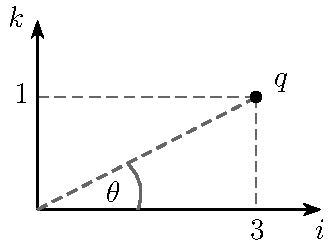
\includegraphics[width=0.3\linewidth]{Figures/quaternion01.pdf}
		\caption{Representa\c c\~ao de $ \lambda = 3\qi + \qk $ no plano $ \qi \qk $.}
		\label{fig:quat3ik}
	\end{figure}
	
%	Utilizaremos a propriedade de rota\c c\~ao da parte vetorial de quat\'ernios, em (\ref{eq:rotacao}).
	Uma vez que o plano $ \qi \qk $ \'e ortogonal a $ \qj $ (lembrando que os tr\^es eixos s\~ao orientados positivamente), a rota\c c\~ao desejada neste plano, positivamente orientada em torno de $ \qj $ e obtida por inspe\c c\~ao da Fig. \ref{fig:quat3ik}, \'e realizada pelo quat\'ernio
	\begin{equation}
	\label{eq:04}
	v = e^{\qj \alpha}, \quad 2\alpha = \theta = \tan^{-1} \frac{1}{3},
	\end{equation}
	utilizando o mapeamento $ \lambda \mapsto v \lambda v^{-1} $ em (\ref{eq:rotacao}).
	
	Uma vez que a transforma\c c\~ao desejada \'e $ \lambda \mapsto q^{-1} \lambda q $, ent\~ao
	\begin{equation}
	%\label{key}
	q = v^{-1} = e^{- \qj \alpha} = e^{- \qj \frac{\theta}{2}}.
	\end{equation}
	
	%It is a known property that ({\color{red}(retirado do artigo ``quat\'ernio rotation intuition'' do math.stack\-exchange, buscar melhor fonte!)}) ``if $ v = e^{\qmu \alpha} = \cos \alpha + \qmu \sin \alpha$, then the mapping $ x \mapsto v x v^{-1} $ will rotate purely imaginary quat\'ernios around the axis $ \mathbb{R} \qmu $ by the angle $ 2\alpha $ according to the right-hand rule''.
	
	Como forma de confer\^encia, encontremos o valor de $ \alpha $ que resulta em $ q^{-1} \lambda q \in \mathbb{C}_{\qi} $. Como $ v = q^{-1} = \cos \alpha + \qj \sin \alpha $,
	\begin{equation}
	%\label{key}
	\begin{aligned}
	%\label{key}
	q^{-1} \lambda &= (\cos \alpha + \qj \sin \alpha)(3 \qi + \qk)\\
	&= \qi(3 \cos \alpha + \sin \alpha) + \qk(\cos \alpha - 3 \sin \alpha). \\
	q^{-1} \lambda q &= [\qi(3 \cos \alpha + \sin \alpha) + \qk(\cos \alpha - 3 \sin \alpha)] (\cos \alpha - \qj \sin \alpha) \\
	&= \qi (3 \cos 2\alpha + \sin 2\alpha) + \qk(\cos 2\alpha - 3 \sin 2\alpha).
	\end{aligned}
	\end{equation}
	
	Portanto, $ q^{-1} \lambda q \in \mathbb{C}_{\qi} $ se e somente se
	\begin{equation}
	%\label{key}
	\begin{aligned}\textbf{}
	\cos 2\alpha - 3 \sin 2\alpha &= 0 \\
	2\alpha &= \tan^{-1} \frac{1}{3},
	\end{aligned}
	\end{equation}
	como inferido em (\ref{eq:04}).
	
Assim, o quat\'ernio puro unit\'ario $ q = e^{- \qj \alpha} $, $ \alpha = - \displaystyle \nicefrac{1}{2} \tan^{-1} \nicefrac{1}{3} $, \'e capaz de fazer $ q^{-1} \lambda q \in \mathbb{C}_{\qi}$, de modo que a equa\c c\~ao de autovalor em (\ref{eq:03}) pode ser reescrita como em (\ref{eq:02}),
	\begin{equation}
	%\label{key}
	\mathbf{A} \underbrace{\begin{pmatrix}
		cos \alpha + \qi \sin \alpha - \qj \sin \alpha - \qk \sin \alpha \\
		2 \sin \alpha + \qi \sin \alpha + \qj 2 \cos \alpha + \qk \cos \alpha
		\end{pmatrix}}_{= \mathbf{v} q} =
	(\mathbf{v} q) \cdot \underbrace{\qi (3 \cos 2\alpha + \sin 2\alpha)}_{= q^{-1} \lambda q}.
	%\underbrace{3.162 \qi}_{= \bar{u} q u}.
	\end{equation}
\end{example}
\end{quotation}

\subsection{Diagonalizabilidade}
\label{subsec:autovetores_XA}

Quanto ao problema de determinar se uma matriz quaterni\^onica \'e \emph{diagonaliz\'avel}, h\'a que se observar que, diferentemente do caso complexo, ter todos os autovalores distintos n\~ao \'e condi\c c\~ao suficiente para diagonalizabilidade. Tomemos o contra-exemplo dado por Zhang \cite[Exemplo 7.4]{zhang1997quaternions}, a matriz
\begin{equation}
\mathbf{A} =
\begin{pmatrix}
\qi & 1\\ 
0 & \qj
\end{pmatrix}.
\end{equation}

Embora possua autovalores distintos -- $ \qi $ e $ \qj $, pois s\~ao as entradas diagonais de uma matriz triangular --, os respectivos autovetores da matriz $ \mathbf{A} $ n\~ao formam um conjunto linearmente independente. Pode-se verificar, por exemplo, que um autovetor associado a $ \qi $ \'e $ (1, 0)^T $, enquanto um associado a $ \qj $ \'e $ (\qi + \qj, 0)^T $. A raz\~ao deles serem linearmente dependentes \'e o fato, mencionado anteriormente, de que para todo autovalor e autovetor $ \lambda $ e $ \mathbf{v} $ de uma matriz quaterni\^onica, tem-se $ q^{-1}\lambda q $ e $ \mathbf{v}q $ como outros autovalor e autovetor, com $ q \in \mathbb{H}^\ast $. Ou seja, dois autovalores \emph{similares} est\~ao sempre associados aos mesmos autovetores, a menos de um fator de escala. Por isso, quat\'ernios similares s\~ao ditos pertencentes \`a mesma \emph{autoclasse} \cite{de2000right}. Para que o conjunto de autovetores associados aos autovalores distintos de uma matriz quaterni\^onica sejam linearmente independentes, portanto, estes autovalores \textbf{n\~ao} podem ser similares.  Concluindo o exemplo dado, pode-se mostrar que $ \qi $ e $ \qj $ s\~ao similares: $ \qj = q \qi q^{-1} $, para $ q \in \{ a - a\qi - a\qj + a\qk \ | \ a\in \mathbb{R}^\ast \} $.

O teorema \ref{th:02} relaciona a autodecomposi\c c\~ao de uma matriz e de sua complexa adjunta, fornecendo um princ\'ipio \'util para o estudo da autoestrutura de matrizes quaterni\^onicas.


\begin{figure}
\centering
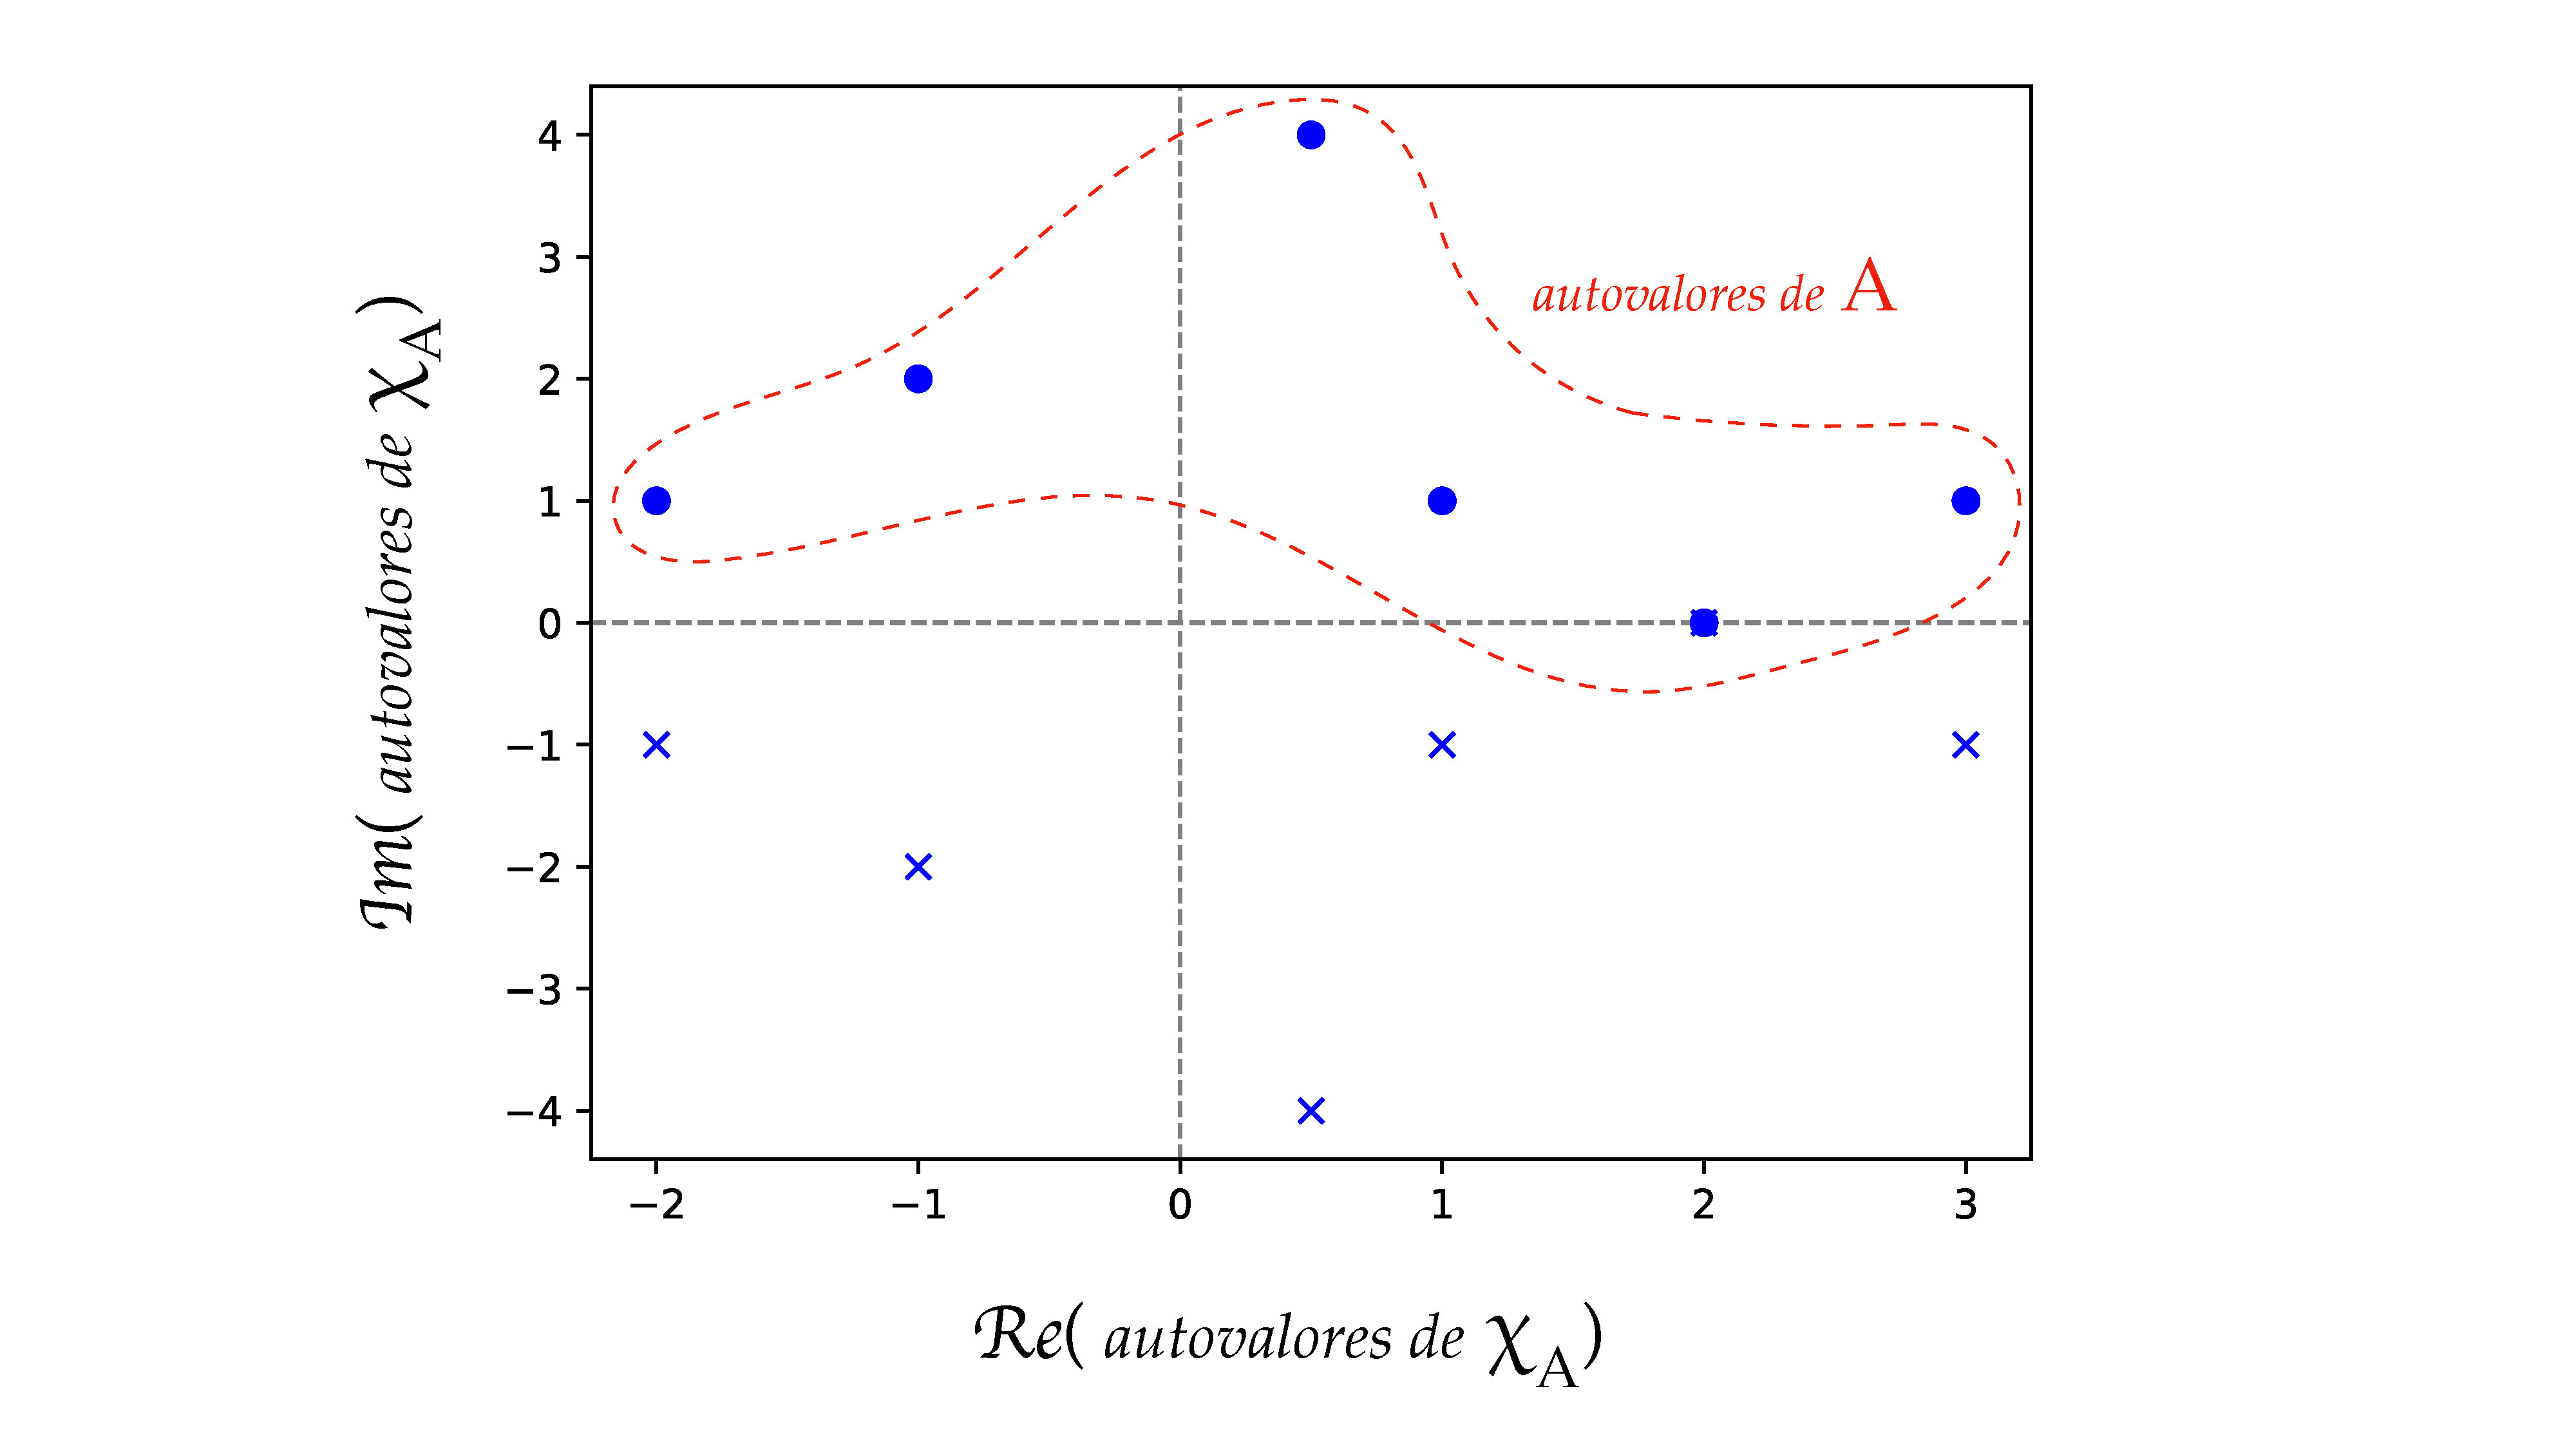
\includegraphics[width=0.6\linewidth]{Figures/complex_adjoint_eigvals_PT.pdf}
\caption{\emph{Autovalores padrão} de uma matriz $ \mathbf{A} $ quaterni\^onica, indicados como um subconjunto dos autovalores de sua respectiva matriz complexa adjunta.}
\end{figure}


\begin{theorem}[\cite{zhang1997quaternions}]
\label{th:02}
Toda matriz $ A \in \mathbb{H}^{n \times n} $ tem exatamente $ n $ autovalores complexos
%(\`a direita),
%que s\~ao iguais aos autovalores de $ \rchi_A $, sua complexa adjunta,
com parte imagin\'aria n\~ao-negativa. Estes s\~ao ditos os \emph{autovalores padr\~ao} de $ \mathbf{A} $ e s\~ao um subconjunto dos $ 2n $ autovalores de $ \rchi_A $.
\end{theorem}

\begin{proof}
Como demonstrado no ap\^endice \ref{ch:AppendixA}, a partir da equa\c c\~ao de autovalor quaterni\^onica
\begin{equation}
\mathbf{A} \mathbf{v} = \mathbf{v} \lambda
\end{equation}
em que se pode assumir, sem perda de generalidade, que $ \lambda \in \mathbb{C} $, pode-se chegar \`a equa\c c\~ao equivalente
\begin{equation}
\begin{pmatrix}
\mathbf{A}_1 & \mathbf{A}_2\\ 
- \overline{\mathbf{A}}_2 & \overline{\mathbf{A}}_1
\end{pmatrix}
\begin{pmatrix}
\mathbf{v}_1 \\ 
- \overline{\mathbf{v}}_2
\end{pmatrix} =
\begin{pmatrix}
\mathbf{v}_1 \\ 
- \overline{\mathbf{v}}_2
\end{pmatrix}
\lambda,
\end{equation}
envolvendo apenas vari\'aveis complexas (i.~e. as componentes da decomposi\c c\~ao de simpl\'etica de $ \mathbf{A} $ e $ \mathbf{v} $). Uma vez que
\begin{equation}
\rchi_A = 
\begin{pmatrix}
\mathbf{A}_1 & \mathbf{A}_2\\ 
- \overline{\mathbf{A}}_2 & \overline{\mathbf{A}}_1
\end{pmatrix}
\end{equation}
\'e uma matriz complexa $ 2n \times 2n $, ela possui $ 2n $ autovalores complexos (distintos ou não). Segundo \cite[Teorema 5]{lee1948eigenvalues}, seus autovalores ocorrem na forma de $ n $ pares conjugados e, por isso, a matriz $ \mathbf{A} $ possui exatamente $ n $ autovalores complexos com parte imagin\'aria n\~ao-negativa.

Os demais autovalores s\~ao redundantes. Seja $ q \in \mathbb{C}_{\qi}$ um destes autovalores. Podemos mostrar que $ q \sim \overline{q} $, pois obt\'em-se $ \overline{q} $ atrav\'es de uma rota\c c\~ao da parte imagin\'aria de $ q $ de 180$ ^\circ $ em torno do eixo $ \qj $. Utilizando o racioc\'inio exposto na subse\c c\~ao \ref{subsec:rotacionando}, com o quat\'ernio $ v = e^{\qj \frac{\pi}{2}} = \qj $ (logo $ v^{-1} = e^{- \qj \frac{\pi}{2}} = -\qj $) e o mapeamento $ q \mapsto v q v^{-1} $,
\begin{equation}
\begin{aligned}
v q v^{-1} &= \qj (q_r + q_i \qi) (-\qj) = q_r - q_i \qj \qi \qj\\
&= q_r + q_i \qi \qj \qj = q_r - q_i \qi = \overline{q}.
\end{aligned}
\end{equation}
Como dois autovalores conjugados de $ \rchi_A $ s\~ao similares, eles pertencem \`a mesma autoclasse e apontam para o mesmo conjunto linearmente dependente de autovetores. Assim, pode-se tomar sempre aquele com parte imagin\'aria nula ou n\~ao-negativa, por conven\c c\~ao.
\end{proof}

O teorema a seguir \'e outro resultado fundamental relacionando a autoestrutura de uma matriz quaterni\^onica e a de sua complexa adjunta.

\begin{theorem}[Teorema 7.4 em \cite{zhang1997quaternions}]
\label{th:diagonal}
Dadas as matrizes $ \mathbf{A}, \mathbf{B} \in \mathbb{H}^{n \times n} $, ent\~ao $ \mathbf{A} $ \'e similar a $ \mathbf{B} $ se, e somente se, $ X\rchi_A $ \'e similar a $ \rchi_B $.
\end{theorem}

\begin{corollary}
Uma matriz $  \mathbf{A} \in \mathbb{H}^{n \times n} $ \'e diagonaliz\'avel se, e somente se, $ \rchi_A $ \'e diagonaliz\'avel.
\end{corollary}
\begin{proof}
Se $ \mathbf{A} \in \mathbb{H}^{n \times n} $ \'e diagonaliz\'avel, ent\~ao \'e similar a uma matriz diagonal $ \Lambda \in \mathbb{C}^{n \times n}_{\qi} $ contendo seus autovalores padr\~ao. Do teorema \ref{th:diagonal}, segue que $ \rchi_A $ \'e similar a
\begin{equation}
\label{eq:Xlambda}
\rchi_{\Lambda} =
\begin{pmatrix}
\Lambda & \mathbf{0}\\ 
\mathbf{0} & \overline{\Lambda}
\end{pmatrix},
\end{equation}
que tamb\'em \'e uma matriz diagonal. Portanto, $ \rchi_A $ \'e diagonaliz\'avel.

Por outro lado, se $ \rchi_A $ \'e diagonaliz\'avel, ent\~ao \'e similar a uma matriz diagonal contendo os seus $ 2n $ autovalores, que aparecem em $ n $ pares complexos conjugados. Assim, sua matriz de autovalores pode ser escrita como (\ref{eq:Xlambda}), o que implica, pelo teorema \ref{th:diagonal}, que $ \mathbf{A} $ \'e similar a $ \Lambda $.
\end{proof}

\section{Laying the foundations for QGSP}

\subsection{On the inversion of the eigenvector matrix}

The inversion of quaternion matrices have been tackled by many researchers, yielding a few algorithms aiming at solving it. \red{(INSERT REFERENCES)} All seemed too costly to practical use in medium to large graphs. Based on theorems \ref{th:equiv01} and \ref{th:equiv02},
the algorithm \ref{alg:qinv} is proposed to provide a reasonable balance between processing speed and broad applicability.

The reasoning goes as follows. According to theorem \ref{th:equiv02}, a sufficient condition for the invertibility of a matrix $\mathbf{V} \in \mathbb{H}^{n \times n}$ is the existance of $\rchi^{-1}_{V}$. Moreover, from theorem \ref{th:equiv01}, if $\rchi^{-1}_{V}$ has the form of a complex adjoint matrix, let us say $\rchi_{V}^{-1} = \rchi_{M}$, then it follows that $\mathbf{M} = \mathbf{V}^{-1}$, since the theorem guarantees that,
\begin{equation}
\rchi_{V} \rchi_{V}^{-1} = \mathbf{I}_{2n \times 2n} = \rchi_{I_{n \times n}} = \rchi_{V} \rchi_{M}
\Rightarrow \mathbf{V} \mathbf{M} = \mathbf{I}_{n \times n},
\end{equation}
letting $\mathbf{I}_{m \times m}$ be the identity matrix of order $m$. For simplicity, this notation is slightly loose, representing both a complex- and a quaternion-valued identity matrix, since in both cases their entries have zero-valued or zero-normed imaginary parts.

\begin{center}
\begin{algorithm}
\caption{Inversion of quaternion matrices.}\label{alg:qinv}
\SetKwInOut{Input}{input}\SetKwInOut{Output}{output}
\Input{$\mathbf{V} \in \mathbb{H}^{n \times n}$}
\Output{$\mathbf{V}^{-1}$ ou None (vazio).}
$\rchi_{V} \gets \mathrm{complex\_adjoint(\mathbf{V})}$\;

\If{$\mathrm{det}(\rchi_{V}) = 0$}{\Return None}

$\mathbf{U} \gets \mathrm{inverse(\rchi_{V})}$

\If{\textup{\textbf{not}} $\mathrm{has\_complex\_adjoint\_form}(\mathbf{U})$}{\Return None}

$\mathbf{V}^{-1} \gets \mathrm{from\_complex\_adjoint}(\mathbf{U})$

\Return $\mathbf{V}^{-1}$
\end{algorithm}
\end{center}

%\section{Poss\'iveis aplica\c c\~oes de QGSP}
%
%Grafos de imagens RGBA, v\'ideos?
%
%Grafos com sinais tridimensionais, como de dire\c c\~ao de vento.

\chapter[Considera\c c\~oes finais]{Considera\c c\~oes finais}
\label{ch:others}

Este projeto de tese prop\~oe-se a contribuir com o processamento de sinais quaterni\^onicos, em particular pelo estudo da autodecomposi\c c\~ao de matrizes quaterni\^onicas, sejam elas matrizes de transforma\c c\~oes lineares ou operadores de deslocamento sobre grafos com pesos quaterni\^onicos. O estudo da autoestrutura da QDFT levou a um novo m\'etodo para sua fracionariza\c c\~ao, juntamente com a proposta de uma vers\~ao multiparam\'etrica e um esquema de cifragem de imagens coloridas com camada de opacidade. A decomposi\c c\~ao de matrizes que servem como operadores de deslocamento para sinais sobre grafos deve ser revelada, em parte, pelos estudos conduzidos at\'e o momento, reunindo teoremas relacionando propriedades destas matrizes e de suas complexas adjuntas, bem como sobre a exist\^encia e similaridade entre autovalores de matrizes sobre os quat\'ernios.

Dentre os desafios te\'oricos que permanecem, pode-se listar os seguintes:
\begin{itemize}
\item encontrar classes de grafos com operadores de deslocamento diagonaliz\'aveis. De fato, enquanto um grafo n\~ao-direcionado com pesos reais ou complexos possui um operador de deslocamento sempre diagonaliz\'avel, n\~ao se pode afirmar o mesmo quando os pesos percentem a $ \mathbb{H} $, pois a simetria presente na matriz de adjac\^encia de um grafo quaterni\^onico n\~ao-direcionado n\~ao se transmite \`a sua matriz complexa adjunta. Neste sentido, pretende-se investigar se h\'a classes de grafos com operadores de deslocamento diagonaliz\'aveis, ou se \'e poss\'ivel definir operadores com tal propriedade. Este problema alinha-se com o entendimento de \cite{ortega2018graph}, que observam forte interesse da comunidade em avan\c cos te\'oricos de GSP voltados a \emph{classes espec\'ificas} de grafos.
\item Ainda nesta linha, pode-se investigar se h\'a quaisquer propriedades particulares presentes na classe de grafos quaterni\^onicos que possuem \emph{apenas autovalores reais} (i.~e. cada autoclasse possui apenas um elemento e o grafo possui um n\'umero finito de autovalores). Em GSP, esta propriedade \'e observada, por exemplo, nos grafos n\~ao-direcionados de pesos reais.
\item Por fim, outra quest\~ao de estudo em aberto \'e como definir um ordenamento das frequ\^encias quando os autovetores s\~ao quaterni\^onicos, pois ainda n\~ao est\'a claro se \'e poss\'ivel transpor a interpreta\c c\~ao oriunda da varia\c c\~ao total sobre grafos, em (\ref{eq:var_total}), para o contexto quaterni\^onico.
\end{itemize}
%est\'a o problema de encontrar classes de grafos com operadores de deslocamento diagonaliz\'aveis. De fato, enquanto um grafo n\~ao-direcionado com pesos reais ou complexos possui um operador de deslocamento sempre diagonaliz\'avel, n\~ao se pode afirmar o mesmo quando os pesos percentem a $ \mathbb{H} $, pois a simetria presente na matriz de adjac\^encia de um grafo quaterni\^onico n\~ao-direcionado n\~ao se transmite \`a sua matriz complexa adjunta. Neste sentido, pretende-se investigar se h\'a classes de grafos com operadores de deslocamento diagonaliz\'aveis, ou se \'e poss\'ivel definir operadores com tal propriedade. Este problema alinha-se com o entendimento de \cite{ortega2018graph}, que observam forte interesse da comunidade em avan\c cos te\'oricos de GSP voltados a \emph{classes espec\'ificas} de grafos. Ainda nesta linha, pode-se investigar se h\'a quaisquer propriedades particulares presentes na classe de grafos quaterni\^onicos que possuem \emph{apenas autovalores reais} (i.~e. cada autoclasse possui apenas um elemento e o grafo possui um n\'umero finito de autovalores). Por fim, outra quest\~ao de estudo em aberto \'e como definir um ordenamento das frequ\^encias quando os autovetores s\~ao quaterni\^onicos, pois ainda n\~ao est\'a claro se \'e poss\'ivel transpor a interpre\c c\~ao oriunda da varia\c c\~ao total sobre grafos, em (\ref{eq:var_total}), para o contexto quaterni\^onico.

%\red{Ler estas fontes e comentar \cite{yin2019quaternion, hsu2018quatnet, parcollet2019quaternion}}

%De posse de um acabou\c co b\'asico de an\'alise espectral e filtragem em QGSP, pretende-se implementar os algoritmos e estruturas de dados em \emph{software}.
Um arcabou\c co coeso de QGSP deve encontrar aplica\c c\~oes em cen\'arios envolvendo sinais que guardem informa\c c\~oes em tr\^es ou quatro dimens\~oes, como dados de dire\c c\~ao de fluidos, imagens coloridas ou rota\c c\~oes de objetos no espa\c co tridimensional. O uso de quat\'ernios pode melhorar a performance em alguns problemas que, hoje, s\~ao atacados com GSP tradicional, tal como ocorreu com aplica\c c\~oes de redes neurais convolucionais \emph{quaterni\^onicas}. Estudos mostraram resultados iguais ou superiores a esquemas com redes convolucionais tradicionais em problemas de processamento e classifica\c c\~ao de imagens coloridas \cite{yin2019quaternion, parcollet2019quaternion}, bem como estima\c c\~ao de pose a partir apenas de imagens em RGB \cite{hsu2018quatnet}. Um exemplo para aplica\c c\~ao de QGSP seria o uso de grafos para predi\c c\~ao de movimento ou compress\~ao de nuvens de pontos (\textit{point clouds}) com informa\c c\~ao espacial e de cor. Em \cite{thanou2016graph}, nuvens de pontos com informa\c c\~ao de cor e posi\c c\~ao no espa\c co 3D s\~ao modeladas como um grafo sobre o qual se define seis sinais distintos (tr\^es de posi\c c\~ao e tr\^es de cor). Utiliza-se de an\'alise espectral para extrair \emph{features} sobre cada um destes sinais, de forma independente, de modo a utiliz\'a-las para estima\c c\~ao de movimento e compress\~ao das nuvens de pontos. Ora, pode-se afirmar sem d\'uvida alguma que tais sinais n\~ao s\~ao independentes e a modelagem utilizando QGSP poderia prover um processamento hol\'istico, eventualmente com maior capacidade de compress\~ao. Em \cite{batabyal2015ugrasp}, os autores representam pontos do corpo humano como v\'ertices de um grafo 3D, com pesos das arestas relacionados \`a dist\^ancia euclidiana entre estes pontos, e utilizam-no para extrair vari\'aveis de entrada para algoritmos de aprendizado de m\'aquina. Cada amostra do sinal sobre o grafo \'e uma tripla ordenada $ s_i = (x_i, y_i, z_i) $, indicando a posi\c c\~ao do v\'ertice no espa\c co. Este sinal, originalmente composto por elementos em $ \mathbb{R}^3 $, \'e representado pelos autores como $ \hat{\mathbf{s}} = [x_1, \dots, x_N, y_1, \dots, y_N, z_1, \dots, z_N] \in \mathbb{R}^{3N}$, ao mesmo tempo em que se define a extens\~ao da matriz $ \mathbf{U} $ de autovetores da Laplaciana: $ \mathbf{U}_g = \text{diag}(\mathbf{U}, \mathbf{U}, \mathbf{U}) $, de modo a se poder utilizar GSP tradicional. O uso de grafos e sinais quaterni\^onicos poderia prover um modelo que naturalmente explora o sinal na sua forma original.


\section{Publica\c c\~oes}

A pesquisa descrita neste projeto de tese gerou, at\'e agora, os trabalhos listados abaixo. O artigo \emph{``Eigenstructure and fractionalization of the quaternion discrete Fourier transform''}, publicado na revista Optik, cont\'em os resultados expostos no cap\'itulo \ref{ch:FrQDFT}. O artigo \emph{``The Cosine Number Transform: A Graph Signal Processing Approach''}, apresentado na confer\^encia GlobalSIP de 2019, surgiu durante estudos paralelos, tamb\'em na linha de generalizar GSP para outras estruturas alg\'ebricas, envolvendo grafos com pesos sobre corpos finitos.

\begin{itemize}
\item Ribeiro, G. B., e Lima, J. B. ``Eigenstructure and fractionalization of the quaternion discrete Fourier transform.'' \emph{Optik} (2019): 163957. DOI: \href{https://doi.org/10.1016/j.ijleo.2019.163957}{10.1016/j.ijleo.2019.163957}

\item Ribeiro, G. B., e Lima, J. B. ``The Cosine Number Transform: A Graph Signal Processing Approach''. 2019 IEEE Global Conference on Signal and Information Processing (GlobalSIP) (pp. 1-5). IEEE. DOI: \href{https://doi.org/10.1109/GlobalSIP45357.2019.8969165}{10.1109/GlobalSIP45357.2019.8969165}
\end{itemize}